\documentclass[12pt, twoside, openany]{report}
\usepackage[dvips]{graphicx,color,rotating}
\usepackage[utf8]{inputenc}
\usepackage{t1enc}
\usepackage{a4wide}
\usepackage{amsfonts}
\usepackage{mathtools}
\usepackage{amsmath}
\usepackage{enumerate}
\usepackage{hyperref}
\usepackage{verbatim}
\usepackage{longtable}
\usepackage[MeX]{polski}
\usepackage[T1]{fontenc}
\usepackage{geometry}
\usepackage{listings}
\usepackage[symbols,nogroupskip,sort=none]{glossaries-extra}
\geometry{left=25mm,right=25mm,bindingoffset=10mm, top=25mm, bottom=25mm}
\usepackage{amssymb, latexsym}
\usepackage{amsthm}
\usepackage{palatino}
\usepackage{array}
\usepackage{pstricks}
\usepackage{comment}
\usepackage{textcomp}
\theoremstyle{definition}
\newtheorem{theorem}{Twierdzenie}[section]
\newtheorem{remark}{Uwaga}[section]
\newtheorem{definition}{Definicja}[section]
\newtheorem{alg}{Algorytm}[chapter]
\newtheorem{prz}{Przypadek}[section]
\newtheorem{np}{Przykład}[section]
\newtheorem{lemma}[theorem]{Lemat}
\linespread{1.5}
\newcommand*{\norm}[1]{\left\Vert{#1}\right\Vert}
\newcommand*{\abs}[1]{\left\vert{#1}\right\vert}
\newcommand*{\om}{\omega}

\renewcommand*{\figureautorefname}{Rys.}
\renewcommand*{\tableautorefname}{Tab.}
\renewcommand*{\chapterautorefname}{rozdz.}
\renewcommand*{\sectionautorefname}{rozdz.}

\usepackage{graphicx}

\author{Marek Szweda}
\title{Poprawa jakości obrazów cyfrowych poprzez metodę wmalowywania}

\makeatletter
\newcommand*\bigcdot{\mathpalette\bigcdot@{.5}}
\newcommand*\bigcdot@[2]{\mathbin{\vcenter{\hbox{\scalebox{#2}{$\m@th#1\bullet$}}}}}
\makeatother

%---lista oznaczeń
\glsxtrnewsymbol[description={przyporządkowanie elementom ze zbioru $a$ elementów ze zbioru $b$}]{rarrow}{$a \rightarrow b$}
\glsxtrnewsymbol[description={}]{wsp1}{$\alpha, \beta, \lambda, \mu$}
\glsxtrnewsymbol[description={}]{wsp2}{$Z, \varepsilon, r, p_s, r$}
\glsxtrnewsymbol[description={parametr, liczba rzeczywista}]{wsp3}{$\Theta$}
\glsxtrnewsymbol[description={wartość piksela obrazu $I$ w punkcie o współrzędnych $(i ,j), x$}]{Iij}{$I_{i,j}, I_{x}$}
\glsxtrnewsymbol[description={wartość piksela obrazu $I$ w punkcie o współrzędnych $i ,j$ w chwili czasu $n+1$}]{Iijn}{$I_{i,j}^{n+1}$}
\glsxtrnewsymbol[description={iloczyn kartezjański zbiorów $a$ i $b$}]{times}{$a \times b$}
\glsxtrnewsymbol[description={pochodna cząstkowa funkcji wielu zmiennych $f$ względem zmiennej $x$}]{frac}{$\frac{\partial f}{\partial x},\frac{\partial f}{\partial_x},\partial{f}_x$}
\glsxtrnewsymbol[description={wartość dyskretnej pochodnej cząstkowej funkcji wielu zmiennych $f$ względem zmiennej $x$ w punkcie o współrzędnych dyskretnych $i, j$}]{fracd}{$\frac{\partial f}{\partial x}\big|_{i,j}, \ \partial f_x \big|_{i,j}$}
\glsxtrnewsymbol[description={pochodna względem czasu $t$}]{fract}{$\frac{\partial }{\partial t}$}
\glsxtrnewsymbol[description={zbiór funkcji kwadratowo całkowalnych}]{squareint}{$L^2(R^2)$}
\glsxtrnewsymbol[description={dywergencja funkcji $f$}]{divf}{$div\left( f \right)$}
\glsxtrnewsymbol[description={wahanie funkcji (ang. total variation)}]{tv}{$TV$}
\glsxtrnewsymbol[description={z ang. non-local color total variation}]{nlctv}{$NLCTV$}
\glsxtrnewsymbol[description={punkt $(i,j)$ obrazu $I$ }]{points}{$x,y,z$}
\glsxtrnewsymbol[description={funkcja wagi, podobieństwo punktów $x,y$ obrazu $I$}]{weight}{$w(x,y)$}
\glsxtrnewsymbol[description={podmacierz wartości obrazu $I$ utworzonych z punktów będących otoczeniem punktu $x$}]{surround}{$I(x+\cdot), p_I(x), p_x, q_x$}
\glsxtrnewsymbol[description={macierz reprezentująca rozkład Gauss'a o odchyleniu standardowym $\sigma$}]{matgauss}{$G_\sigma$}
\glsxtrnewsymbol[description={iloczyn po współrzędnych macierzy $A$ i $B$}]{hadarmatrix}{$A * B$}
\glsxtrnewsymbol[description={dziedzina obrazu $I$ nie podlegająca modyfikacji}]{dziedzina}{$D$}
\glsxtrnewsymbol[description={wypełniana część obrazu $I$}]{wmalowane}{$\Omega$}
\glsxtrnewsymbol[description={reprezentacja funkcji będącej nielokalnym przekształceniem $D \times D \rightarrow R$} w modelu $NLCTV$]{nlreop}{$p$}
\glsxtrnewsymbol[description={normy wektorowe}]{normywektor}{$\ell_{1},\ell_{2}$}
\begin{document}

\def \kotmyszm{obr. nr 1}
\def \maciekIm{obr. nr 2}
\def \ObrIm{obr. nr 3}
\def \ObrIVm{obr. nr 4}
\def \ObrVm{obr. nr 5}
\def \ObrVIm{obr. nr 6}
\def \ObrXVm{obr. nr 7}
\def \ObrXVIIm{obr. nr 8}
\def \ObrXIXm{obr. nr 9}
\def \ObrXXVIIIkm{obr. nr 10}
\def \OsobaDrugam{obr. nr 11}
\def \ObrXIIIm{obr. nr 12}
\def \XXVIII{obr. nr 1}
\def \TEST{obr. nr 2}
\def \Wood{obr. nr 3}

\def \SNRI{obr. nr 1}
\def \SNRII{obr. nr 2}
\def \SNRIII{obr. nr 3}
\def \SNRIV{obr. nr 4}

\begin{titlepage}
\pagestyle{empty}

\noindent
\begin{Large}
\begin{table}[t]
\centering
\begin{tabular}[t]{lcr}

\includegraphics[width=70pt,height=70pt]{rysunki/PW} & POLITECHNIKA WARSZAWSKA & 
\includegraphics[width=70pt,height=70pt]{rysunki/ele}\\
& WYDZIAŁ ELEKTRYCZNY & \\
\end{tabular}
\end{table}

% \vfill
\begin{center}PRACA DYPLOMOWA MAGISTERSKA\end{center}
%\begin{center}MATEMATYKA\end{center}
\end{Large}
% \vfill
\begin{center}
\Huge
\textbf{Poprawa jakości obrazów cyfrowych poprzez metodę wmalowywania}
\end{center}
% \vfill\vfill
\vfill
\begin{center}
\Large
Autor:\\
\LARGE
Marek Szweda
\end{center}
\vfill
\begin{center}
\Large
Promotor: dr Sławomir Skoneczny
\end{center}
\vfill
\begin{center}
\large
Warszawa, listopad 2018
\end{center}
\newpage
\hfill
\begin{table}[b]
\centering
\begin{tabular}[t]{ccc}
............................................. & \hspace*{100pt} & .............................................\\
podpis promotora & \hspace*{100pt} & podpis autora
\end{tabular}
\end{table}


% \maketitle
\end{titlepage}
\thispagestyle{empty}
\newpage
\pagestyle{headings}
\setcounter{page}{1}
\hyphenation{Syl-ves-tra}
\hyphenation{Syl-ves-ter-a}

\begin{abstract}
Tu będzie jakieś streszczenie
\end{abstract}

%-----------Oznaczenia-----------
\newpage
\printunsrtglossary[type=symbols, style=long, title={Wykaz oznaczeń i symboli}]
    
%-----------Poczłtek człłci zasadniczej-----------

\chapter{Wprowadzenie do przetwarzania obrazów.}
W ostatnich latach analiza obrazów zyskuje na popularności ciągle zwiększając swój obszar w dziedzinie badań. Ogólnie proces analizy obrazu można przedstawić następującym modelem: \\
\begin{figure}[!h]
	\centering
	\includegraphics{rysunki/1_fig1.png}
\end{figure}
\\
Jest wiele rodzajów analizy obrazu takich jak model stochastyczny, transformacje, równania różniczkowe wyższego rzędu, analiza funkcjonalna. Jednym z podstawowych problemów w analizie obrazów jest ulepszenie uszkodzonego obrazu. Poprawa jakości poprzez metodę wmalowywania jest szeroko stosowana w aplikacjach do edycji obrazów, usuwania niechcianych obiektów z obrazów, tekstów, zarysowań, uszkodzeń, poprawy starych zdjęć oraz filmów. Przed przejściem do dokładniejszej analizy wmalowywania obrazu należy podać definicje obrazu cyfrowego.
\section{Obraz cyfrowy.}
Dwuwymiarowy obraz jest reprezentacją skończonej ilości dyskretnych wartości zwanych pikselami. Każdy z pikseli przypisany jest do konkretnego położenia w dwuwymiarowej przestrzeni $x = {i,j} \in D=\mathcal{R}^2$, gdzie $D$ oznacza przestrzeń obrazu. Wartość piksela $f(x)$ stanowi informację o natężeniu oraz nasyceniu kolorów w danym punkcie $x$. Najczęściej obraz przechowywany jest jako zbiór wartości $f(x) \in \langle 0,255 \rangle$, gdzie 0 oznacza najmniejszą wartość intensywności, a 255 największą wartość intensywności. Obraz w odcieniach szarości stanowi przekształcenie $f: D \rightarrow \mathcal{R}$. W przypadku obrazów kolorowych obraz stanowi przekształcenie $f: D \rightarrow \mathcal{R}^n$, gdzie $n$ określa ilość przestrzeni barw. Przykładem przestrzeni może być przestrzeń $RGB$, gdzie przy wykorzystaniu trzech kolorów $(n=3)$ uzyskuję się skończoną gammę innych kolorów. Biorąc pod uwagę trzy podstawowe kolory oraz 256 wartości ich intensywności obraz może modelować $256^3=16777216$ różnych kolorów. Jakość obrazu zależy od jego rozdzielczości. Rozdzielczość określa się jako liczbę wierszy i kolumn przypadających na obraz. Obrazy o dużej rozdzielczości charakteryzują się znikomą zdolnością do odróżnienia poszczególnego z pikseli obrazu, dzięki czemu w ogólnym wrażeniu tworzy gładki obraz.
\section{Wmalowywanie obrazów.}
Cyfrowe wmalowywanie obrazu jest artystycznym synonimem zapożyczonym z techniki wykorzystywanej przez profesjonalnych restauratorów odnawiających dzieła sztuki w muzeach. Niech $D$ oznacza całą przestrzeń obrazu będącego przekształceniem $f: D \rightarrow R^{n}$. Problem wmalowania obrazu polega na wypełnieniu pustej części zbioru $\Omega \subset D$ na podstawie informacji znajdującej się na zewnątrz $\Omega$. Do tak zdefiniowanego problemu istnieje wiele rozwiązań przedstawianych w literaturze. Wmalowywanie obrazów definiuje się jako automatyczne wypełnianie braków w obrazie na podstawie otoczenia, w sposób uniemożliwiający obserwatorowi znalezienie pierwotnie wybrakowanych miejsc. Przykłady obrazów poddanych operacji wmalowywania przedstawia \autoref{1_fig1} 
\begin{figure}[!h]
	\centering
	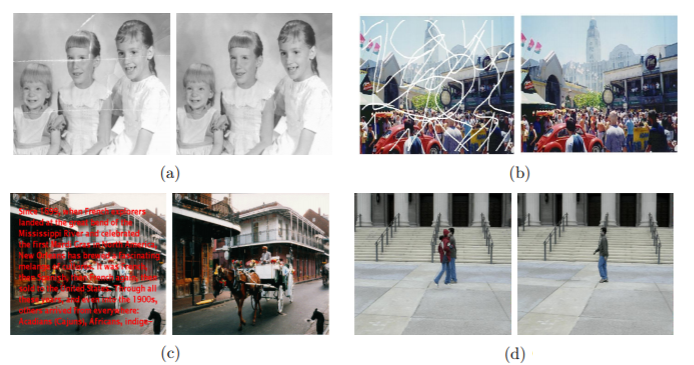
\includegraphics[scale=0.7]{rysunki/fig1}
	\caption{Przykłady obrazów poddanych operacji wmalowywania.}
	\label{1_fig1}
\end{figure}
\par
Obrazy przedstawiono w parze: po lewej obraz wejściowy, po prawej wynikowy obraz poddany operacji wmalowywania. Mogą nimi być uszkodzenia jak w przypadku a oraz b, napisy znajdujące się na obrazie - c, czy też obiekty, którym w konkretnym przypadku d jest postać. Przestrzeń do wmalowywania w obrazie wyznaczana jest manualnie poprzez użytkownika definiującego konkretny obiekt, który powinien według niego zostać usunięty. Program automatycznie nie jest w stanie wyznaczyć części, która powinna zostać przearanżowana. 
Techniki wmalowywania znajdują szeroki zakres zastosowań w przetwarzaniu nagrań filmowych, gdzie nieznany region na scenie musi zostać oszacowany w pewien sposób dostarczając spójności wizualnej użytkownikowi. Przykładami mogą być konieczność ukrywania błędów nagrań, strat wynikających z błędów urządzeń nagrywających, czy też usunięcia niepożądanych obiektów, które w trakcie nagrywania pojawiły się w kadrze. Głównym celem pracy jest osiągniecie algorytmu skutecznie odbudowującego wcześniej zdefiniowaną nieznaną przestrzeń obrazu. W tym celu dokonano przeglądu istniejących algorytmów wmalowywania opartych na rozwiązaniu odpowiednio zdefiniowanych problemów matematycznych. Wyniki badanych zagadnień uzyskiwane są na podstawie danych wejściowych w postaci zdefiniowanych obszarów obrazu otaczających brakujące regiony. Podstawowymi operacjami wykorzystywanymi w bardziej złożonych algorytmach rekonstrukcji są:
\begin{enumerate}
\item
Rozwiązanie cząstkowych równań różniczkowych wyższego rzędu bazujących na kontynuacji tekstur, geometrii, struktur obrazu.
\item
Analiza funkcjonalna, problem minimalizacji energii o szerokim zakresie sposobów definicji.
\item
Wyznaczenie podobieństwa pomiędzy obszarami w obrazie za pomocą wprowadzonej metryki 
\end{enumerate}
W pracy opisano przedstawione powyżej algorytmy, porównano oraz zaproponowano nowy model uzupełniania brakujących danych. Porównania dokonano na podstawie dwóch najistotniejszych właściwości: szybkości algorytmu oraz obiektywnej oceny poprawności otrzymanego wyniku. Zwrócono także uwagę na różne cechy obrazu, które mogą determinować dobór algorytmu do zadanego problemu. Warto zaznaczyć, iż do tej pory nie została przedstawiona jednoznaczna definicja problemu matematycznego pozwalająca w niezawodny sposób wyznaczyć braki w obrazie niezależnie od jego cech charakterystycznych.
\chapter{Przegląd istniejących algorytmów.}
Pierwszą gałęzią algorytmów zgodnie z rozróżnieniem wprowadzonym w  \cite{SalientStrucTexProp} są metody opierające się na rozwiązaniu równań różniczkowych wyższego rzędu. Wśród nich pojawia się próba przystosowania procesu dyfuzji do wypełniania braków w obrazie (źródła \cite{bertalmio2000image} lub \cite{BertalmioNavierStokes}), dzięki której przy wykorzystaniu zależności z działu mechaniki płynu można dokonać próby kontynuacji informacji z otoczenia w brakujące obszary. \\
Drugą gałęzią algorytmów są metody oparte na uzupełnianiu braków obrazu kawałek po fragmencie skopiowanymi częściami istniejącego obrazu z miejsc o najlepszym dopasowaniu w miejsce braku. Pierwszy raz metoda syntezy obrazu kopiowanymi kawałkami została zaproponowana w \cite{efros1999texture}. Kolejność wypełniania braków nie jest obojętna i ma znaczny wpływ na ostateczną spójność obrazu. Jedna z najpopularniejszych metod określania priorytetu została przedstawiona w \cite{criminisi2004region}. Na przestrzeni czasu pojawiło się wiele metod minimalizujących zjawisko niespójności w obrazie takich jak np. \cite{StructurePropagationManual}. \\
Innym sposobem wyznaczenia braków jest analiza funkcjonalna definiująca problem minimalizacji energii stanowiąca największą grupę zdefiniowanych rozwiązań wmalowywania. Przykładem mogą być \cite{MathematicalModelsforNLTextureInpainting}, \cite{ColorTextureInpaintingNLCTVModel}, czy też \cite{arias2011variational}. W przytoczonych przykładach rozwiązanie problemu minimalizacji stanowi wynik w postaci wmalowanego obrazu. Innym przykładem może być problem minimalizacji zdefiniowany w \cite{SalientStrucTexProp} stanowiący pośredni proces w wypełnianiu obrazu. Tu problem minimalizacji, będący segmentacją obrazu, pozwala oddzielić strukturę i teksturę, pozwalając w następstwie na przeprowadzenie oddzielnej syntezy dwóch zbiorów danych, za pomocą róznych algorytmów. \\
Ostatnią grupą algorytmów jest grupa stanowiąca połączenie powyższych algorytmów. Najprostszym przykładem grupy może być przytoczone wcześniej \cite{NavierStokesAndTexturePropagation}, w którym zaproponowano poprzedzenie procesu wmalowywania segmentacją obrazu. Uzyskaną w procesie segmentacji teksturę uzupełnia się metodą najbliższego dopasowania natomiast strukturę uzyskuje na podstawie równań różniczkowych. Kolejnym przykładem może być publikacja \cite{arias2011variational}, w której autorzy proponują nielokalny model wyznaczający nieznany obszar obrazu wykorzystując rachunek wariacyjny, połączony ze zdefiniowaną metryką wyznaczającą odległości pomiędzy rozpatrywanymi fragmentami obrazu. \\
Większość metod wmalowywania opisanych w literaturze opiera się na algorytmach kontynuujących strukturę, geometrię bądź teksturę obrazu. Modele bazujące na geometrii i strukturze w uogólnieniu generują efekt uboczny w postaci braku kontynuacji tekstur, sprawiających wrażenie rozmytego obrazu. Do algorytmów broniących się przed efektem rozmycia można zaliczyć takie, w których wyznaczeniu konkretnego miejsca w nieznanym obszarze może towarzyszyć przebadanie całego zbioru punktów niemodyfikowanej części obrazu. Stąd metody kontynuujące tekstury w większości uważa się za metody nielokalne.
\chapter{Równania mechaniki płynu.}
\label{chap:navierstokes}
\section{Rozwiązanie równania Naviera-Stokesa }
W celu dokładnego zaprezentowania idei wmalowywania w oparciu o równanie Naviera-Stokesa należy rozważyć poniższe równanie przepływu cieczy Newtonowskiej:
\begin{equation}
\mathbf{V}\nabla \mathbf{V}\mathrm{+}\frac{d\mathbf{V}}{dt}\mathrm{=-}\frac{\mathrm{1}}{q}\nabla \mathbf{p}\mathrm{+}\mathbf{F}\mathrm{+}\nu {\nabla }^{\mathrm{2}}\mathbf{V}
\label{NavierStokesEquation}
\end{equation}
\begin{equation}
\mathrm{V=\ (-}\frac{\mathrm{\partial }\mathrm{\Psi }}{\mathrm{\partial }\mathrm{y}},\frac{\mathrm{\partial }\mathrm{\Psi }}{\mathrm{\partial }\mathrm{x}}\mathrm{)}
\label{LiquidVelociy}
\end{equation}
gdzie $V$ oznacza prędkość lokalną, $t$ chwilę czasu, $q$ gęstość lokalną, $p$ ciśnienie lokalne, $F$ siłę zewnętrzną działającą lokalnie na ciecz, $\nu$ lepkość kinematyczną lokalną. $\mathit{\Psi}$ oznacza linię prądu będącą ciągłą linią w polu prędkości płynu, poprowadzoną
stycznie do wektorów prędkości w danej chwili. Człon $V\nabla V$ odpowiada konwekcji lokalnego pędu wraz z ruchem cieczy, $\frac{1}{q}\nabla p$ wpływowi sił ciśnieniowych na zmianę pędu (kompensuje niezerową konwekcję),  $F$ odpowiada sile zewnętrznej działającej na ciecz (np. grawitację) natomiast $\nu {\nabla }^2V\ $ odpowiada dyssypacji pędu cieczy od tarcia pomiędzy cząstkami. Traktując płyn jako nieściśliwy ($q \leftarrow \infty $)  oraz pomijając działanie sił zewnętrznych ($F=0$)  równanie możemy uprościć do postaci:
\begin{equation}
 V\nabla V+\frac{dV}{dt}=\nu {\nabla }^2V
\label{NavierStokesEquationShort}
\end{equation}
Dokonując obustronnej rotacji równania \cite{StreamfuntionVorticityForm} otrzymujemy równanie w zależności od wirowości:
\begin{equation}
V\nabla \omega \mathrm{+}\frac{d\omega }{dt}\mathrm{=}\nu {\nabla }^{\mathrm{2}}V
\label{NavierStokesEquationVorticity}
\end{equation}
przy czym wirowość określa się wzorem:
\begin{equation}
\omega =\nabla \times V
\label{Vorticity}
\end{equation}
Niech $I$ reprezentuje obraz cyfrowy będący macierzą o rozmiarze$m \mathrm{\times} n$, \cite{ebrahimi2012navier}. Wtedy $I_{i,j}$ zawiera wartość dodatnią całkowitą z przedziału od 0 do 255, stanowiącą informację o poziomie jasności danego piksela z obrazu. Wartość 0 opowiada odcieniowi czarnemu, natomiast 255 odcieniowi czystemu białemu. Niech D stanowi zbiór indeksów $(i,j)\ \in \ \left\{1,2\dots ,m\right\} \mathrm{\times}$ $\left\{1,2\dots ,n\right\}$. Obraz $I$ wtedy można traktować jako funkcję $I:D\to R$.
\par
W 2000 roku Bertalmio w \cite{BertalmioNavierStokes} wprowadza analogię pomiędzy wirowością a gładkością obrazu. Dokładniej przedstawia to \autoref{tab1}
\begin{table}[!h]
	\centering
	\begin{tabular}{|cc|c|}
	\hline \hline

		& Navier-Stokes
		& Wmalowywanie w obrazie\\ \hline
		
		& Linia prądu $\ \mathit{\Psi}$ &  Jasność obrazu $I$ \\ \hline
	
		& Prędkość płynu $V = {\mathrm{\nabla }}^{\bot }\mathit{\Psi} = [u, v]$  & Kierunek izotop $V$ = ${\mathrm{\nabla }}^{\bot }I = [u, v]$ \\ \hline
		& Wirowość $\omega =\ {\mathrm{\nabla }}^2\mathit{\Psi}$ & gładkość $\omega =\ {\mathrm{\nabla }}^2I$ \\ \hline
		
		& Lepkość płynu $\nu $ & Parametr dyfuzji anizotropowej $\nu $ \\
	\hline
	\end{tabular}
	\caption{przekształcenie zmiennych w zagadnieniu wmalowywnia obrazu.}
	\label{tab1}
\end{table}
gdzie ${\nabla }^{\bot }=(\frac{\partial }{\partial y},\frac{\partial }{\partial x})$.
Niech $\mathit{\Omega}\subset D$ stanowi wypełniany obszar obrazu (maskę). W wyniku rozwiązania dyskretnego równania Naviera-Stokesa w obszarze maski z warunkami brzegowymi zdefiniowanymi jako jasność pikseli sąsiadujących z obszarem maski uzyskuje się kontynuację linii o podobnej jasności (izolinii) w głąb odrestaurowywanego obszaru zgodnie z \autoref{3_fig1}.  Matematycznie kierunek izolinii jasności obrazu wyznacza ${\nabla }^{\bot }I$. W oparciu o \autoref{tab1} oraz równanie  \eqref{NavierStokesEquationVorticity} zagadnienia wmalowywania można sformułować jako problem stabilnego rozwiązania poniższego równania różniczkowego:
\begin{equation}
{\mathrm{(}\mathrm{\nabla }}^{\mathrm{\bot }}I\mathrm{)}\mathrm{\cdot }\nabla {\mathrm{(}\mathrm{\nabla }}^{\mathrm{2}}I\mathrm{)+}\frac{d{\mathrm{(}\mathrm{\nabla }}^{\mathrm{2}}I\mathrm{)}}{dt}\mathrm{=}\nu \mathrm{\nabla }\mathrm{(}g\mathrm{(}\nabla {\mathrm{(}\mathrm{\nabla }}^{\mathrm{2}}I\mathrm{))}\nabla {\mathrm{(}\mathrm{\nabla }}^{\mathrm{2}}I\mathrm{))} 
\label{NavierStokesInpainting}
\end{equation}
\begin{figure}[!h]
	\centering
	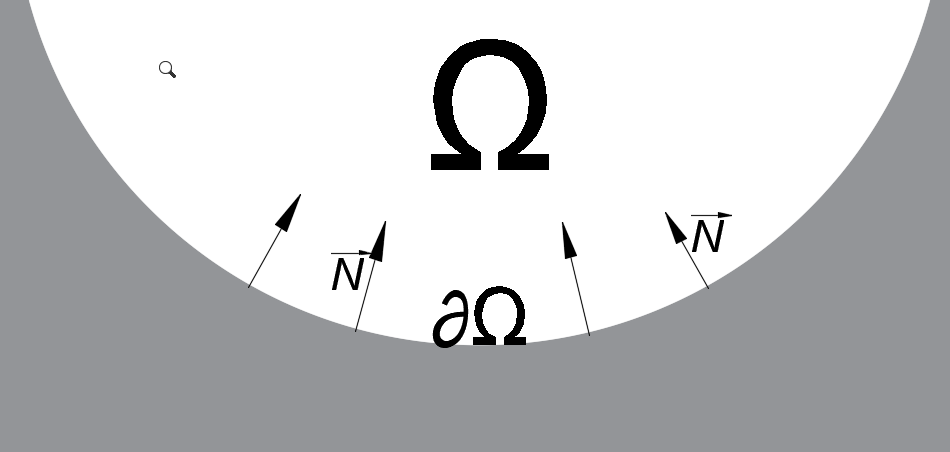
\includegraphics[scale=0.3]{rysunki/3_fig1}
	\caption{Propagacja jasności obrazu wgłąb nieznanego obszaru.}
	\label{3_fig1}
\end{figure}
W równaniu \eqref{NavierStokesInpainting} człon odpowiedzialny za tarcie pomiędzy cząstkami płynu $\nu {\nabla }^2V\ $ został zastąpiony dyfuzją anizotropową, która w kontekście przetwarzania obrazów pierwszy raz wprowadzona została przez Perona i Malika w 1987 roku \cite{perona1990scale}. Dyfuzja anizotropowa ma znaczny wpływ na zachowanie krawędzi obrazu oraz poprawę jego ostrości. Za dyfuzję anizotropową odpowiada współczynnik $g$, który przedstawiany jest w różnych postaciach funkcji przewodności. W tej pracy wykorzystana zostanie postać:
\begin{equation}
g\left(s\right)=\frac{1}{1+\alpha \left|s\right|}
\end{equation}
gdzie $\alpha\ $, $K$ wcześniej zdefiniowane parametry dyfuzji (stałe), ${\mathrm{\nabla }}^{\bot }=({-\partial }_y,{\partial }_x)$. 
Dyskretne rozwiązanie równania \eqref{NavierStokesInpainting} jest analogiczne do dyskretnego rozwiązania przepływu płynu w przestrzeni $2D$. W tym celu należy wprowadzić chwile w czasie $t=n\cdot \Delta t$, gdzie $n=\left\{1,2,3,\dots ,N\right\}$, $\Delta t$ wartość przyrostu czasu pomiędzy dyskretnymi chwilami $n$ i $n+1$, $N$ moment osiągnięcia stanu ustalonego, matematycznie przedstawianego jako:
\begin{equation}
\frac{\partial I}{\partial t}\mathrm{+}{\mathrm{\nabla }}^{\mathrm{\bot }}I\mathrm{\nabla }\mathrm{\Delta }I\mathrm{\ }\mathrm{\cong }\mathrm{0}
\label{NavierStokesStability}
\end{equation}
Warto zauważyć, że człon ${\mathrm{\nabla }}^{\bot }I$ w równaniu \eqref{NavierStokesStability} odpowiada kierunkowi rozchodzenia się punktów o podobnej jasności, natomiast $\mathrm{\nabla }\Delta I$ to kierunek największej zmiany gładkości obrazu. Jeśli wektory są do siebie prostopadłe  iloczyn skalarny wynosi 0 i przedstawia stan stabilny. 
W celu dokładnej analizy dyskretyzacji równanie \eqref{NavierStokesEquationVorticity} zostanie rozdzielone na dwa podrównania:
\begin{equation}
\frac{d{\mathrm{(}\mathrm{\nabla }}^2I)}{dt}=-{\mathrm{(}\mathrm{\nabla }}^{\bot }I)\cdot \nabla {\mathrm{(}\mathrm{\nabla }}^2I)+\left\{ad\right\}
\label{NavierDiffAdv}
\end{equation}
oraz
\begin{equation}
ad=\nu \mathrm{\nabla }(g(\nabla {\mathrm{(}\mathrm{\nabla }}^2I))\nabla {\mathrm{(}\mathrm{\nabla }}^2I))
\label{NavierAdv}
\end{equation}
Rozwiązanie powyższych równań dokonywane będzie na siatce obliczeniowej typu Eulera, a wszystkie wartości wyznaczanych zmiennych będą znajdować się w centrach komórki zdefiniowanej jako konkretny piksel obrazu, zgodnie z \autoref{3_fig1} 
\begin{figure}[!h]
	\centering
	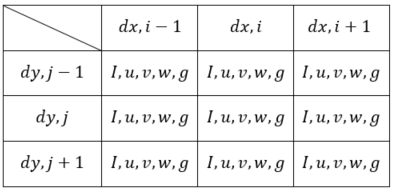
\includegraphics[scale=1.2]{rysunki/fig2}
	\caption{Przykłady obrazów poddanych operacji wmalowywania.}
	\label{3_fig2}
\end{figure}
Równanie \eqref{NavierDiffAdv} to równanie różniczkowe cząstkowe typu parabolicznego. Równanie to  można rozwiązać w sposób przybliżony używając schematu centralnego bądź schematu do przodu. W przypadku równania parabolicznego oba schematy dają stabilne rozwiązanie. W celu ułatwienia dalszych rozważań wprowadzono funkcję $f$ określoną w centrach siatki, z dolnymi indeksami wskazującymi na konkretne miejsce w siatce. Korzystając z rozwinięcia w szereg Taylora możemy gradient funkcji $f$ w punkcie $(i,j)$ przybliżyć następującym wzorem:
\begin{equation}
\nabla f_{i,j}=\left[\ {\frac{\partial f}{\partial x}|}_{i,j,}{\frac{\partial f}{\partial y}|}_{i,j}\right]
\label{gradF}
\end{equation}
gdzie:
\begin{equation}
{\frac{\partial f}{\partial x}} {\bigg |}_{i,j}=\frac{f_{i+1,j}+f_{i-1,j}}{2\Delta x}
\label{dfdx}
\end{equation}
Analogicznie:
\begin{equation}
{\frac{\partial f}{\partial y}} {\bigg |}_{i,j}=\frac{f_{i,j+1}+f_{i,j-1}}{2\Delta y}
\label{dfdy}
\end{equation}
Na podstawie powyższych wzorów składowe wektora ${\mathrm{\nabla }}^{\bot }I$, czyli kierunku, w którym należy propagować gładkość obrazu ${\mathrm{\nabla }}^2I$ wyznacza się z zależności:
\begin{equation}
u_{i,j}=\frac{I_{i,j+1}+I_{i,j-1}}{2\Delta y} 
\label{u}
\end{equation}
Oraz
\begin{equation}
 v_{i,j}=-\frac{I_{i+1,j}+I_{i-1,j}}{2\Delta x}
\label{v}
\end{equation}
Przy czym:
\begin{equation}\\
{\mathrm{\nabla }}^{\bot }I=|-u,v|
\label{gradI}
\end{equation}
Stosując pięciopunktowy analog różnicowy w metodzie różnic skończonych operator Laplace’a dla przyjętej siatki Eulera można przybliżyć wzorem (przy założeniu, że $\Delta x=\ \Delta y$):
\begin{align}
\begin{aligned}
{\mathrm{\nabla }}^2f_{i,j} &= \Delta f_{i,j}=\\[1ex]
&={\frac{{\partial }^2f}{\partial x^2}}\bigg|_{i,j}+{\frac{{\partial }^2f}{\partial y^2}}\bigg|_{i,j}=\\
&=\frac{f_{i+1,j+1}+f_{i-1,j+1}+f_{i+1,j-1}+f_{i-1,j-1}-4f_{i,j}}{\Delta x^2}\ 
\end{aligned}
\label{LaplaceOpr}
\end{align}
Korzystając z wyznaczonych powyżej zależności na wartości $u$ oraz $v$ wartość gładkości obrazu $\omega =\ {\mathrm{\nabla }}^2I$ można przedstawić w postaci: 
\begin{equation}
\Delta {I}\big|_{i,j}=\ {\frac{\partial v}{\partial x}}\bigg|_{i,j,}-\ {\frac{\partial u}{\partial y}}\bigg|_{i,j}
\label{discreteVorticity}
\end{equation}
Podobnie jak w przypadku liczenia pochodnej w dziedzinie obrazu pierwszą pochodną w dziedzinie czasu przybliża się rozwinięciem w szereg Taylora. Niech indeks górny oznacza konkretną chwilę czasową. Wtedy wartość pochodnej wynosi:
\begin{equation}
\ {{\frac{\partial f}{\partial t}}\bigg|^n_{i,j}=\ \frac{f^{n+1}_{i,j}-\ f^n_{i,j}}{\Delta t}}
\label{dfdt}
\end{equation}
Ostatecznie rozwiązanie dyskretnego równania parabolicznego \eqref{NavierDiffAdv} , gdzie $\Delta x= \Delta y=h$, z wykorzystaniem schematu centralnego ma postać:
\begin{align}
{\omega }^{n+1}_{i,j} &= {\omega }^n_{i,j}+\Delta t\biggl[
-\left(\frac{I_{i,j+1}+I_{i,j-1}}{2h}\right)\left(\frac{{\omega }_{i+1,j}
+{\omega }_{i-1,j}}{2h}\right)+\notag\\ 
&\qquad+ \left(\frac{I_{i+1,j}+I_{i-1,j}}{2h}\right)\left(\frac{{\omega }_{i,j+1}+{\omega }_{i,j-1}}{2h}\right)+{\left\{ad\right\}}_{i,j} \biggr]
\label{NavierDiffAdvCen}
\end{align}
Rozwiązanie równania \eqref{NavierDiffAdv} można przedstawić również w drugiej postaci wykorzystującej schemat „do przodu”, charakteryzujący się wyznaczaniem wartości pochodnej wirowości w zależności od wyznaczonego kierunku ${\mathrm{(}\mathrm{\nabla }}^{\bot }I)$.  Wtedy równanie \eqref{NavierDiffAdvCen} przyjmuje postać:
\begin{align}
\fontsize{11}
{\omega }^{n+1}_{i,j} &= {\omega }^n_{i,j}+\Delta t\biggl[
-\left(\frac{I_{i,j+1}+I_{i,j-1}}{2h}\right)\left(\frac{{\omega }_{k,j}+{\omega }_{i,j}}{2h}\right)+ \notag\\ 
&\qquad+ \left(\frac{I_{i+1,j}+I_{i-1,j}}{2h}\right)\left(\frac{{\omega }_{i,l}+{\omega }_{i,j}}{2h}\right)+{\left\{ad\right\}}_{i,j} \biggr]
\label{NavierDiffAdvFor}
\end{align}
gdzie:
\begin{align}
k = i+sgn\left(u^n\right) \\
l = j+sgn(u^n)
\end{align}
\par
Rozwiązanie równania \eqref{NavierAdv}, w którym zastąpiono postać zwykłej dyfuzji $\nu {\nabla }^2V$ wymaga uważniejszego potraktowania ze względu na większą podatność na niestabilność implementowanych metod dyskretyzacji. Równanie to można przedstawić w postaci dywergencji pola wektorowego uzyskanego w wyniku wyliczenia gradientu wirowości z uwzględnionym współczynnikiem dyfuzji anizotropowej:
\begin{align}
\begin{aligned}
\left\{ad\right\} 
&= \nu \mathrm{\nabla }(g(\nabla {\mathrm{(}\mathrm{\nabla }}^2I))\nabla {\mathrm{(}\mathrm{\nabla }}^2I)= \\[1ex]
&= \nu \mathrm{\nabla }\mathrm{\cdot}(g(|\nabla \omega |)\nabla \omega )=\\[1ex]
&= {\partial }_x\left(g\left(\left|\nabla \omega \right|\right){\partial }_x\omega \right)+{\partial }_y\left(g\left(\left|\nabla \omega \right|\right){\partial }_y\omega \right)
\end{aligned}
\label{Anisotropic}
\end{align}
\eqref{Anisotropic}
gdzie: ${\partial }_x=\frac{\partial }{\partial x}$ oraz analogicznie: ${\partial }_y=\frac{\partial }{\partial y}$.
Zgodnie z \cite{ebrahimi2012navier} powyższe równanie można rozwiązać w poniższych krokach:
Korzystając z zależności \eqref{dfdx} i \eqref{dfdy} należy wyznaczyć wartości ${\frac{d\omega }{dx}}\big|_{i,j}$ oraz ${\frac{d\omega }{dy}}\big|_{i,j}$
Na podstawie wartości z punktu 1 należy obliczyć moduł wektora w przestrzeni Euklidesowej:
\begin{equation}
{\left|\mathrm{\nabla }\omega \right|}_{i,j}=\ \sqrt{\frac{\partial \omega }{\partial x}\bigg|^2_{i,j}+\frac{\partial \omega }{\partial y}\bigg|^2_{i,j}}
\label{magnitudedw}
\end{equation}
Na podstawie wartości z punktu 2 należy wyznaczyć wartość $g{\left({\left|\mathrm{\nabla }\omega \right|}_{i,j}\right)}$ wykorzystując \eqref{NavierStokesInpainting}. Korzystając z wartości wyznaczonych powyżej oraz ponownie z zależności \eqref{dfdx} i \eqref{dfdy} trzeba obliczyć:
\begin{align}
\{ad_{i,j}\} &= \partial_x \left( g(\left| \nabla\omega \right|_{i,j}) \cdot \partial_x \omega \big|_{i,j} \right) \bigg|_{i,j} \notag +\\[1ex]
&+ \partial_y \left( g(\left|\nabla\omega\right|_{i,j}) \cdot \partial_y \omega \big|_{i,j} \right)\bigg|_{i,j}
\label{discreteAnisotropic}
\end{align}
\par
Innym sposobem dyskretyzacji równania \eqref{NavierAdv} może być metoda przedstawiona w \cite{van2005algorithms}, wykorzystująca asymetryczny schemat liczenia pierwszej pochodnej funkcji. Pierwsze pochodne lewostronne przyjmują postać:
\begin{equation}
\frac{\partial^-f}{\partial x}\bigg|_{i,j}=\frac{f_{i,j}+f_{i-1,j}}{\Delta x}
\label{leftdfdx}
\end{equation}
\begin{equation}
{\frac{{\partial }^-f}{\partial y}}\bigg|_{i,j}=\frac{f_{i,j}+f_{i,j-1}}{\Delta y}
\label{leftdfdy}
\end{equation}
Analogicznie prawostronne:
\begin{equation}
{\frac{{\partial }^+f}{\partial x}}\bigg|_{i,j}=\frac{f_{i+1,j}+f_{i,j}}{\Delta x} 
\label{rightdfdx}
\end{equation}
\begin{equation}
{\frac{{\partial }^+f}{\partial y}}\bigg|_{i,j}=\frac{f_{i,j+1}+f_{i,j}}{\Delta y}
\label{rightdfdy}
\end{equation}
Następnie powyższe zależności znajdują zastosowanie w wyznaczeniu wyrażeń\\ ${\partial }_y\left(g\left(\left|\nabla \omega \right|\right){\partial }_y\omega \right)$ oraz ${\partial }_x\left(g\left(\left|\nabla \omega \right|\right){\partial }_x\omega \right)+{\partial }_y$. Stosując naprzemiennie schemat lewostronny i prawostronny do liczenia wartości pochodnych wewnętrznych i zewnętrznych w wyniku otrzymuje się ogólny schemat centralny. Stosując powyższe ostatecznie równanie \eqref{NavierAdv} można przedstawić w następującej postaci dyskretnej:
\begin{align}
\begin{aligned}
{\left\{ad\right\}}_{i,j}
&= \frac{1}{2}\biggl[\left(g_{i,j}+g_{i+1,j}\right)\left({\omega }_{i+1,j}-{\omega }_{i,j}\right) -\\[1ex]
&- \left(g_{i-1,j}+g_{i,j}\right)\left({\omega }_{i,j}-{\omega }_{i-1,j}\right) +  \\[1ex]
&+ \left(g_{i,j}+g_{i,j+1}\right)\left({\omega }_{i,j+1}-{\omega }_{i,j}\right) -\\[1ex]
&- \left(g_{i,j-1}+g_{i,j}\right)\left({\omega }_{i,j}-{\omega }_{i,j-1}\right)\biggl]
\end{aligned}
\label{discreteAnisotropic2}
\end{align}
Należy zauważyć, iż do wyznaczenia wartości $u$, $v$ oraz ${\mathrm{\nabla }}^2I$ wykorzystywanych do obliczeń \eqref{NavierDiffAdv} i \eqref{NavierAdv} w każdej kolejnej chwili czasu $n$, konieczna jest znajomość obrazu $I^n$. W związku z tym równocześnie z równaniem \eqref{Vorticity} należy rozwiązywać poniższe niejednorodne równanie różniczkowe cząstkowe liniowe drugiego rzędu.
\begin{equation}
\Delta I^n={\omega }^n
\label{Poisson}
\end{equation}
Dla przestrzeni dwuwymiarowej równanie przyjmuje postać:
\begin{equation}
\frac{{\partial }^2I}{\partial x^2}+\frac{{\partial }^2I}{\partial y^2}=\ \omega
\label{Poisson2D}
\end{equation}
W celu przybliżenia drugiej pochodnej funkcji $f$ w punkcie $(i,j)$ należy rozwinąć funkcję $f$ w dwa szeregi Taylora względem punktu $(i+1,j)$ oraz $(i-1,j)$. Po rozwiązaniu sumy dwóch rozwinięć względem $\frac{{\partial }^2f}{\partial x^2}$ otrzymuje się poniższy sposób dyskretyzacji drugiej pochodnej:
\begin{equation}
{\frac{{\partial }^2f}{\partial x^2}\bigg|}_{i,j}\mathrm{=}\frac{f_{i+1,j}-2f_{i,j}+f_{i-1,j}}{\Delta x^2}
\label{d2fdx2}
\end{equation}
Analogicznie:
\begin{equation}
{\frac{{\partial }^2f}{\partial y^2}\bigg|}_{i,j}\mathrm{=}\frac{f_{i,j+1}-2f_{i,j}+f_{i,j-1}}{\Delta y^2}
\label{d2fdy2}
\end{equation}
Korzystając z \eqref{d2fdx2} oraz \eqref{d2fdy2} równanie \eqref{Poisson} w punkcie $(i,j)$ przyjmuje postać pięciopunktowego analogu różnicowego operatora $\Delta $ ($\Delta x=\ \Delta y=h)$:
\begin{equation}
I_{i+1,j}+I_{i-1,j}+I_{i,j+1}+I_{i,j-1}-4I_{i,j}=h^2{\omega }_{i,j}
\label{Laplace}
\end{equation}
Na podstawie równania \eqref{Laplace} można stworzyć równanie macierzowe postaci $Ax=B$, gdzie $x$ reprezentuje obraz $I$, $B$ gładkość obrazu, natomiast $A$ to macierz charakterystyczna współczynników. Istnieje wiele metod rozwiązywania równań Poissona takich jak metoda Jacobiego czy Gaussa-Seidla.  Wystarczającą wydajność i szybkość działania w celach rozwiązania równania można uzyskać stosując metodę SOR – sukcesywnej nadrelaksacji, \cite{blacksuccessive}. Dyskretyzacja równania wygląda następująco:
\begin{align}
\begin{aligned}
I^{n+1}_{i,j}
&= \left(1-\ \beta \right)I^n_{i,j}+\beta \cdot \frac{1}{2}{\left(\frac{1}{\Delta x^2}+\frac{1}{\Delta y^2}\right)}^{-1} \cdot \\[1ex]
&\cdot \left[\frac{1}{\Delta x^2}{(I}^n_{i+1,j}+I^{n+1}_{i-1,j})+\frac{1}{\Delta y^2}{(I}^n_{i,j+1}+I^{n+1}_{i,j-1})+{\omega }^n_{i,j}\right]
\end{aligned}
\label{DiscreteSOR}
\end{align}
Metoda w swoim równaniu przyjmuje parametr wagowy $\beta$ odpowiadający za zbieżność algorytmu. Dobór parametrów nie jest losowy i $\beta$ zawiera się w przedziale $(0,2)$. Zgodnie z \cite{blacksuccessive} parametr ten powinno przyjmować się zgodnie z zależnością \cite{ancona2002computational}:
\begin{equation}
{\omega }_{opt}=2{\left(1+\frac{\pi }{N}\right)}^{-1}
\label{BetaChoose}
\end{equation}
gdzie $N$ to liczba kolumn przyjętej siatki obliczeniowej. 
\par
Operacje wmalowywania bardzo często wykonywane są w punktach maski tworzących nieregularne kształty, mogących znajdować się w różnych częściach obrazu. Stąd powyżej przedstawiony schemat obliczeń wykonywany jest dla wszystkich pikseli obrazu. Po każdej iteracji uzyskane wartości $I^{n+1}$ w znanych punktach przepisywane są z oryginalnego obrazu $I^{0}$, zgodnie z zależnością poniżej.
\begin{equation}
I^{n+1}(D/\mathrm{\Omega }\mathrm{)\ }\ ={\ I}^0(D/\mathrm{\Omega }\mathrm{)}
\label{retrieveMask}
\end{equation}
\par
Podsumowując w celu wyznaczenia nieznanych wartości obrazu w punktach zdefiniowanych przez maskę należy powtarzać następujące kroki do uzyskania stanu ustalonego:
\begin{enumerate}
\item
Rozwiązać równanie \eqref{discreteAnisotropic} 
\item
Na podstawie równania \eqref{NavierDiffAdvCen} zamiennie z \eqref{NavierDiffAdvFor} wyznaczyć wartości $\omega_{i,j}^{n+1}$ dla każdego punktu $(i,j)$ 
\item
Korzystając z \eqref{DiscreteSOR} wyznaczyć jasność każdego piksela $I_{i,j}^{n+1}$.
\item
Do uzyskanego obrazu w punkcie 3 przepisać znane wartości z obrazu oryginalnego
\end{enumerate}
Powyższy algorytm przedstawiono dla obrazów w odcieniach szarości $I:D\to R$. W przypadku obrazów kolorowych, zdefiniowanych funkcją będącą przekształceniem w pole wektorowe $[R,G,B]$, czyli $I:D\to R^3$ metodę stosuje się oddzielnie dla każdej z warstwy. Zgodnie z propozycją przedstawioną w \cite{fishelov2006image} obraz można również przekształcić w poprzedzającym algorytm kroku do współrzędnych sferycznych (CIELab) $\left[I_{1},I_{2},I_{3} \right]$ zgodnie z zależnościami:
\begin{equation}
{I_{1_{i,j}}=r}_{i,j}=\ \sqrt{R^2_{i,j}+G^2_{i,j}+B^2_{i,j}}
\label{TIone}
\end{equation}
\begin{equation}
I_{2_{i,j}}=\ {\mathrm{sin} {\mathrm{\Theta }}_{i,j}\ }=\ {\mathrm{sin} {{\mathrm{tan}}^{-1} \frac{G_{i,j}}{R_{i,j}}\ }\ } 
\label{TItwo}
\end{equation}
\begin{equation}
I_{3_{i,j}}=\ {\mathrm{sin} {\phi }_{i,j}\ }=\ {\mathrm{sin} {{\mathrm{cos}}^{-1} \frac{B_{i,j}}{r_{i,j}}\ }\ } 
\label{TIthree}
\end{equation}
Następnie dysponując składowymi $I_1$, $I_2$, $I_3$ wyznaczonymi z powyższych zależności, dla każdego z nich oddzielnie należy wykonać wcześniej opisane iteracje. W celu odwrotnego przekształcenia $\left[I_1,I_2,I_3 \right]\to\left[R,G,B\right]$ wystarczy wykonać poniższe obliczenia:
\begin{equation}
 B_{i,j}=\ r_{i,j}{\mathrm{cos} {\mathrm{\Theta }}_{\mathrm{i,j}}\ }{\mathrm{cos} {\phi }_{\mathrm{i,j}}\ }
\label{TInvIone}
\end{equation}
\begin{equation}
R_{i,j}=\ r_{i,j}{\mathrm{cos} {\mathrm{\Theta }}_{\mathrm{i,j}}\ }{\mathrm{sin} {\phi }_{\mathrm{i,j}}\ }
\label{TInvItwo}
\end{equation}
\begin{equation}
G_{i,j}=\ r_{i,j}{\mathrm{sin} {\theta }_{\mathrm{i,j}}\ } 
\label{TInvIthree}
\end{equation}
Operację wmalowywania można wykonać na pierwotnych składowych $[R,G,B]$ lecz matematyczna transformacja przestrzeni charakteryzuje się lepszymi właściwościami związanymi z postrzeganiem różnicy barw $\delta E$ przez ludzkie oko:
\begin{equation}
\Delta E=\ \sqrt{{\Delta I_1}^2+{\Delta I_2}^2+{\Delta I_3}^2}
\label{deltaE}
\end{equation}
\chapter{Analiza funkcjonalna.}
\section{Wmalowywanie struktury i tekstury obrazu.}\label{chap:StructureTextureNavierStokes}
\subsection{Segmentacja obrazu na strukturę i teksturę.}
Metoda jednoczesnego wmalowywania struktur i tekstur pierwszy raz przedstawiona została przez Bertalmio i innych w 2003 roku w \cite{NavierStokesAndTexturePropagation}. Opiera się ona na wmalowywaniu struktury w oparciu o algorytm przedstawiony w artykule przy jednoczesnej propozycji prostej syntezy tekstury. Niech $I$ oznacza obraz $R^2\to R,\ \ I\in L^2(R^2)$. Proces wypełniania brakującego regionu $\mathrm{\Omega }$ poprzedzony jest dekompozycją obrazu:
\begin{align}
I\left(i,j\right)=u\left(i,j\right)+v\left(i,j\right) 
\label{STRUCTURETEXTURE1}
\end{align}
uzyskaną na podstawie rozwiązania problemu minimalizacji energii:
\begin{align} 
{\mathop{\mathrm{min}}_{u} \Biggl\{E\left(u\right)=\int{\left|\mathrm{\nabla }u\right|+\lambda {\left|\left|v\right|\right|}^2_{L^2}}\Biggr\}\ }
\label{STRUCTURETEXTURE2}
\end{align}
gdzie: $\int{\left|\mathrm{\nabla }u\right|}$ stanowi funkcjonał z przestrzeni o ograniczonym wahaniu $BV(R^2)$ pozwalający usunąć z oryginalnego obrazu szum i powtarzające się w małej skali detale, przy jednoczesnym zachowaniu głównych cech oraz ostrych krawędzi, ${\left|\left|v\right|\right|}^2_{L^2}$ to człon odpowiadający dokładności odwzorowania, $\lambda $ stanowi wcześniej zdefiniowany parametr. Dla odpowiednio małych wartości $\lambda $ problem minimalizacji prowadzi do uzyskania jednorodnego komponentu $u$ reprezentującego odfiltrowany obraz oraz komponentu $v$ reprezentującego wahania w postaci szumu oraz tekstur. Zgodnie z dowodem Mayera w przypadku gdy pożądany jest wspomniany kształt funkcji $v$, można udowodnić jej  przynależność do przestrzeni Banacha oznaczanej przez $G$. W związku z tym (pomijając wyprowadzenia) problem minimalizacji można przedstawić w ostatecznej postaci minimalizacji energii:
\begin{align}
\begin{aligned} 
\mathop{\mathrm{min}}_{u,g_1,g_2} \Biggl\{E &= \int{\left|\mathrm{\nabla }u\right|+\lambda \int{{\left|I-u-{\partial }_xg_1-{\partial }_yg_2\right|}^2dxdy}} \\
&+ \mu {\left[\int{{\sqrt{g^2_1+g^2_2}}^\beta dxdy}\right]}^{\frac{1}{\beta}}\Biggr\}
\end{aligned}
\end{align}
gdzie:
\begin{align}
v=div\left(\mathop{g}\right),\ \mathop{g}=\left[g_1,g_2\right],\ g_1=-\frac{1}{2\lambda }\frac{u_x}{\left|\mathrm{\nabla }u\right|},\ g_2=-\frac{1}{2\lambda }\frac{u_y}{\left|\mathrm{\nabla }u\right|}\
\label{VG1G2}
\end{align}
oraz $\beta \to \mathrm{\infty }$. Stosując podstawowe równanie rachunku wariacyjnego postaci równania Eulera-Lagrange'a uzyskuje się odpowiadające mu postacie funkcji wykorzystywane do minimalizacji energii:
\begin{align}
u=I-u-{\partial }_xg_1-{\partial }_yg_2+\frac{1}{2\lambda }div\left(\frac{\mathrm{\nabla }u}{\left|\mathrm{\nabla }u\right|}\right)
\end{align}
\begin{align}
{\mu H\left(g_1,g_2\right)g}_1=2\lambda \left[\frac{\partial }{{\partial }_x}\left(u-I\right)+{\partial }^2_{xx}g_1+{\partial }^2_{xy}g_2\right]
\end{align}
\begin{align}
\mu H\left(g_1,g_2\right)g_2=2\lambda \left[\frac{\partial }{{\partial }_y}\left(u-I\right)+{\partial }^2_{xy}g_1+{\partial }^2_{yy}g_2\right]
\end{align}
gdzie $\mu$ stanowi wcześniej definiowany parametr dyskretyzacji, natomiast $H\left(g_1,g_2\right)$ opisane jest wzorem:
\begin{align}
H\left(g_1,g_2\right)={{{\left|\left|\sqrt{g^2_1+g^2_2}\right|\right|}_\beta}^{1-\beta}}{\left(\sqrt{g^2_1+g^2_2}\right)}^{\beta-2}
\end{align}
Zgodnie z zaleceniami podanymi w \cite{vese2003modeling} w celach dyskretyzacji parametr $\beta$ przyjęto równy 1, ze względu na brak znaczących różnic wyniku w przypadku stosowania większych wartości. Wtedy:
\begin{align}
H\left(g_1,g_2\right)=\frac{1}{\sqrt{g^2_1+g^2_2}}
\end{align}
Formalnie, jedno z równań Eulera-Lagrange'a uzyskiwanych podczas minimalizacji wspomnianej energii $E$ ma postać:
\begin{align}
u=I+\frac{1}{2\lambda }div\left(\frac{\mathrm{\nabla }u}{\left|\mathrm{\nabla }u\right|}\right)
\end{align}
Stąd można wywnioskować, że:
\begin{align}
v=-\frac{1}{2\lambda }div\left(\frac{\mathrm{\nabla }u}{\left|\mathrm{\nabla }u\right|}\right)
\end{align}
Korzystając z zależności występujących jako \eqref{VG1G2} możemy łatwo zauważyć, że spełnione jest $g^2_1+g^2_2=\frac{1}{2\lambda }$. Stąd:
\begin{align}
H\left(g_1,g_2\right)=\sqrt{2\lambda }
\end{align}
\begin{align}
u=I-u-{\partial }_xg_1-{\partial }_yg_2+\frac{1}{2\lambda }div\left(\frac{\mathrm{\nabla }u}{\left|\mathrm{\nabla }u\right|}\right)
\label{EU}
\end{align}
\begin{align}
\mu \sqrt{2\lambda }g_1=2\lambda \left[\frac{\partial }{{\partial }_x}\left(u-I\right)+{\partial }^2_{xx}g_1+{\partial }^2_{xy}g_2\right]
\label{EG1}
\end{align}
\begin{align}
\mu \sqrt{2\lambda }g_2=2\lambda \left[\frac{\partial }{{\partial }_y}\left(u-I\right)+{\partial }^2_{xy}g_1+{\partial }^2_{yy}g_2\right]
\label{EG2}
\end{align}
Jako wartości początkowe tego iteracyjnego algorytmu można przyjąć:
\begin{align}
u^0=f,\ g_1=-\frac{1}{2\lambda }\frac{f_{\mathrm{x}}}{\left|\mathrm{\nabla }f\right|},\ g_2=-\frac{1}{2\lambda }\frac{f_{\mathrm{y}}}{\left|\mathrm{\nabla }f\right|}
\end{align}
Następnie stosując zależności wyznaczania pochodnych \eqref{dfdx}, \eqref{dfdy}, \eqref{leftdfdx}, \eqref{leftdfdy} oraz poniższą metodę aproksymacji pochodnej drugiego stopnia:
\begin{align}
\begin{aligned} 
{\partial }_{xy}g_1 \big|_{i,j} &\cong \frac{1}{2h^2} \bigg[2g_1\big|_{i,j}+g_1\big|_{i-1,j-1}+g_1\big|_{i+1,j+1}-g_1\big|_{i,\ j-1} -\\ 
&-g_1\big|_{i-1,j}-g_1\big|_{i+1,j}-g_1\big|_{i,j+1}\bigg]
\end{aligned}
\end{align}
możemy równania \eqref{EU}, \eqref{EG1} i \eqref{EG2} przedstawić w następującej postaci dyskretnej:
\begin{align}
\begin{aligned}
u^{n+1}\big|_{i,j} &= \left[\frac{1}{1 + \left(\frac{1}{2\lambda h^2}\right)\cdot \left(c_1\big|_{i,j}+c_2\big|_{i,j}+c_3\big|_{i,j}+c_4\big|_{i,j}\right)}\right]\bigcdot \\ 
&\bigcdot \biggl[I\big|_{i,j}- \left(\frac{g^n_1\big|_{i+1,j}\cdot g^n_1\big|_{i-1,j}}{2h}\right)- \left(\frac{g^n_2\big|_{i,j+1}-g^n_2\big|_{i,j-1}}{2h}\right) +\\ 
&+\ \left(\frac{1}{2\lambda h^2}\right)\bigcdot \Bigl[c_1\big|_{i,j}\cdot u^n\big|_{i+1,j}+c_2\big|_{i,j}\cdot u^n\big|_{i-1,j} +\\
&+c_3\big|_{i,j}\cdot \lambda \cdot {u}^n\big|_{i,j+1}+c_4\big|_{i,j}\cdot u^n\big|_{i,j-1}\Bigr]\biggr]
\end{aligned}
\end{align}
\begin{align}
\begin{aligned}
g^{n+1}_1\big|_{i,j} &= \left[\frac{2\lambda }{\mu \sqrt{2\lambda }+\ 4\frac{\lambda }{2h}}\right]\bigcdot \Biggl[\frac{u^n\big|_{i+1,j}-u^n\big|_{i-1,j}}{2h}-\frac{I\big|_{i+1,j}-I\big|_{i-1,j}}{2h}+\\
&+\frac{g_1\big|_{i+1,j}+g_1\big|_{i-1,j}}{h^2}\frac{1}{2h^2}\cdot \Bigl[2g^n_2\big|_{i,j}+ g^n_2\big|_{i-1,j-1} +\\ 
&+ g^n_2\big|_{i+1,j+1}+
g^n_2\big|_{i,j-1}-g^n_2\big|_{i-1,j}+g^n_2\big|_{i+1,j}-\\
&-g^n_2\big|_{i,j+1}\Bigr]\Biggr]
\end{aligned}
\end{align}
\begin{align}
\begin{aligned}
g^{n+1}_2\left(i,j\right) &=\left[\frac{2\lambda }{\mu \sqrt{2\lambda }\ +\ 4\frac{\lambda }{2h}}\right]\bigcdot \Biggl[\frac{u^n\big|_{i,j+1}-u^n\big|_{i,j-1}}{2h}-\frac{I\big|_{i,j+1}-I\big|_{i,j-1}}{2h}+\\ 
&+\frac{g_2\big|_{i,j+1}+g_2\big|_{i,j-1}}{h^2}+\frac{1}{2h^2}\cdot \Bigl[2g^n_1\big|_{i,j}+ g^n_1\big|_{i-1,j-1}+ g^n_1\big|_{i+1,j+1} -\\
&-\ g^n_1\big|_{i,j-1}-g^n_1\big|_{i-1,j}+g^n_1\big|_{i+1,j}- g^n_1\big|_{i,j+1}\Bigr]\Biggr]
\end{aligned}
\end{align}
przy czym:
\begin{align}
\begin{aligned}
c^n_1\big|_{i,j}=\frac{1}{\sqrt{{\left(\frac{u^n\big|_{i+1,j}-u^n\big|_{i,j}}{h}\right)}^2+ {\left(\frac{u^n\big|_{i,j+1}-u^n\big|_{i,j-1}}{2h}\right)}^2+\ \varepsilon }}
\end{aligned}
\end{align}
\begin{align}
\begin{aligned}
c^n_2\big|_{i,j}=\frac{1}{\sqrt{{\left(\frac{u^n\big|_{i,j}-u^n\big|_{i-1,j}}{h}\right)}^2+ {\left(\frac{u^n\big|_{i-1,j+1}-u^n\big|_{i-1,j-1}}{2h}\right)}^2+\ \varepsilon }}
\end{aligned}
\end{align}
\begin{align}
\begin{aligned}
c^n_3\big|_{i,j}=\frac{1}{\sqrt{{\left(\frac{u^n\big|_{i+1,j}-u^n\big|_{i-1,j}}{2h}\right)}^2+\ {\left(\frac{u^n\big|_{i,j+1}-u^n\big|_{i,j}}{h}\right)}^2+\ \varepsilon }}\end{aligned}
\end{align}
\begin{align}
\begin{aligned}
c^n_4\big|_{i,j}=\frac{1}{\sqrt{{\left(\frac{u^n\big|_{i+1,j-1}-u^n\big|_{i-1,j-1}}{2h}\right)}^2+\ {\left(\frac{u^n\big|_{i,j}-u^n\big|_{i,j-1}}{h}\right)}^2+\ \varepsilon }}
\end{aligned}
\end{align}
W celu uniknięcia problemu dzielenia przez zero w powyższej dyskretyzacji wprowadzono parametr $\varepsilon \longrightarrow 0$. 
Po przeprowadzeniu powyższej segmentacji obrazu dla uzyskanych członów $u$ i $v$ można zastosować różne algorytmy wmalowywania braków. Autorzy w \cite{NavierStokesAndTexturePropagation} proponują aby do wmalowywania struktur zastosować algorytm przedstawiony w \cite{bertalmio2000image}, natomiast do uzyskania brakującej tekstury sugerują użycie następującego algorytmu syntezy obszaru $\mathrm{\Omega }$ \\:
\begin{figure}[!h]
	\centering
	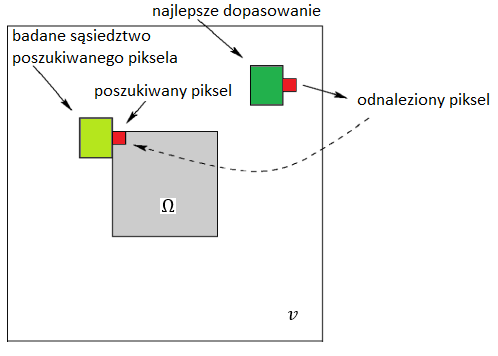
\includegraphics[scale=1]{rysunki/5_fig1}
	\caption{Prosty algorytm wmalowywania tekstury obrazu.}
	\label{5_fig1}
\end{figure} \\
Zgodnie z \autoref{5_fig1} dla każdego piksela znajdującego się na granicy $\mathrm{\Omega }$ tworzone jest okno stanowiące szablon wykorzystywany do odnalezienia najlepszego dopasowania z pośród całego obrazu $v$. W przypadku odnalezienia takiego dopasowania uzyskany piksel kopiowany jest w miejsce poszukiwanego piksela. Algorytm ten można wykonywać pobierając piksele z granicy w kolejności zgodnej z kolejnością obrotu wskazówek zegara, postępując w głąb obszaru $\mathrm{\Omega }$, aż do wypełnienia wszystkich brakujących pikseli. 
W przypadku obrazów kolorowych $I$ w przestrzeni $[R, G, B]$ wypełnianie można poprzedzić wykonaniem przekształcenia $I$ zgodnie z zależnościami \eqref{TIone}, \eqref{TItwo} i \eqref{TIthree} ze względu na ich lepsze właściwości. Następnie każda z trzech uzyskanych warstw jest rozbijana na własną teksturę i strukturę. W przypadku algorytmu dokonującego syntezy tekstury oddzielnie dla każdej z 3-ech segmentowanych warstw uzyskiwane wyniki charakteryzują się pojawiającymi się niespójnościami kolorów. Stąd w przypadku odrestaurowywania uzyskanych części $v$, zlokalizowanie piksela będącego najlepszym dopasowaniem aktualnie badanego, nieznanego piksela, odbywa się na podstawie pierwszej warstwy, a wszystkie trzy warstwy uzupełniane są analogicznie do obliczeń uzyskanych na podstawie pierwszej warstwy. Kroki algorytmu można przedstawić następująco:
\begin{enumerate}
\item
Przekształcenie warstw $R,G,B$ obrazu na współrzędne sferyczne $I_1,I_2,I_3$.
\item
Wyznaczenie $u_1,v_1,\ u_2,v_2,u_3,v_3$ na podstawie $I_1,I_2,I_3$.
\item
Wmalowanie nieznanych obszarów $\mathrm{\Omega }$ w warstwach $u_1,u_2,u_3$ dowolnie dobraną metodą.
\item
Wmalowanie obszaru $\mathrm{\Omega }$ w $v_1,v_2,v_3$ na podstawie dowolnego algorytmu syntezy tekstury $v_1$.
\end{enumerate}
\section{Model NLCTV. (Non-local color total variation)}
Pojęcie wahania funkcji $TV$ (total variation)w analizie obrazów pierwszy raz wprowadzone zostało przez Rudin, Osher i Fatemi’ego w \cite{rudin1992nonlinear}, gdzie proponowany model znajduje zastosowanie w usuwaniu szumów z obrazu. Następnie model $TV$ zostaje zaproponowany do wmalowywania obrazu w \cite{MathematicalModelsforNLTextureInpainting} przez Chan i Shen’a. Problem doboru parametrów dla modelu $TV$, właściwości oraz proces dyskretyzacji problemu minimalizacji jest dokładnie przedstawiony w \cite{getreuer2012total}. Algorytm bazujący na lokalnych funkcjonałach $TV$  charakteryzuje się zdolnością do kontynuacji geometrycznych struktur obrazu i krawędzi. Zgodnie z przedstawioną literaturą wadą algorytmu jest brak możliwości propagacji tekstury w nieznany obszar $\Omega$. Warto wspomnieć, iż w przypadku usuwania szumów z obrazów wykorzystanie operatorów lokalnych nie pozwala zachować tekstur. Problem jednoczesnej propagacji geometrii i tekstury można rozwiązać przy zastosowaniu modelu nielokalnego, który zostanie poddany analizie w niniejszej pracy. \\
Klasyczny nielokalny model wahania funkcji został intensywnie przebadany dla obrazów w odcieniach szarości. W przypadku obrazów kolorowych jednym z pierwszych zaproponowanych modeli jest model Mumford-Shah dokładnie opisany w \cite{jung2011nonlocal}. Model ten dla każdej z warstw obrazu kolorowego przeprowadza oddzielną analizę, prowadząc do niejednorodnego kontrastu kolorów obrazu w przestrzeni wmalowywanej $\Omega$ z jego otoczeniem $D/\mathrm{\Omega}$. Problem uzyskania jednakowego kontrastu rozwiązano poprzez propozycję nowego, szybkiego modelu przedstawionego w \cite{duan2015fast} wprowadzającego zależność pomiędzy wszystkimi warstwami obrazu kolorowego. W celu analizy nowego, nielokalnego modelu wahania funkcji dla obrazów kolorowych $NLCTV$ (z ang. non-local color total variation) zaproponowanego w \cite{duan2015fast} należy wcześniej wprowadzić oznaczenia i zależności operatorów nielokalnych. 
Zgodnie z poprzednim działem niech $D$ stanowi dziedzinę obrazu. Wtedy obraz w odcieniach szarości możemy przedstawić jako wynik przekształcenia $I\left(x\right):D\longrightarrow R,\ x\in R$ zdefiniowaną dla każdego piksela $x$ ze zbioru $D$. Wtedy pojęcie nielokalnego gradientu pomiędzy pikselem $x$ i $y$, gdzie $x,y\in D$ z definicji możemy wyrazić zależnością:
\begin{equation}
{\mathrm{\nabla }}_{NL}I\left(x,y\right)\triangleq \left[I\left(y\right)-I\left(x\right)\right]\sqrt{w(x,y)}
\label{NLGRAD}
\end{equation}
Warto zauważyć, że wynikiem powyższej zależności nie jest wektor, a wartość skalarna. Wyrażenie stanowi proste przekształcenie $D \times D\longrightarrow R$. Wartość wagi $w(x,y)$ z definicji wyraża się poniższą zależnością:
\begin{equation}
w\left(x,y\right)\triangleq {\mathrm{exp} \left\{-\frac{G_{\sigma }*{\left|I\left(x+\ \cdot \right)-I\left(y+\ \cdot \right)\right|}^2}{r^2}\right\}\ }
\label{NLWEIGHT}
\end{equation}
\begin{figure}[!h]
	\centering
	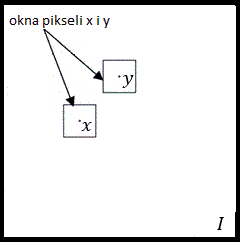
\includegraphics[scale=1]{rysunki/3_fig3.png}
	\caption{Kształt okien wykorzystywanych do obliczania wartości $w(x,y)$.}
	\label{3_fig3}
\end{figure}
Wartość $r$ to zdefiniowana wcześniej stała skalująca wartości podobieństwa pomiędzy pikselami. Podobieństwo wyznaczane jest na podstawie utworzonych okien scentrowanych względem piksela $x$ oraz $y$ oznaczanych operatorem "$\cdot$" zgodnie z \autoref{3_fig3}. Normę macierzową występującą w powyższej zależności można wyznaczyć korzystając z normy Frobeniusa:
\begin{equation}
{\|I\left(x+\cdot \right)-I\left(y+\cdot \right)\|}=\ \sum^{p_s}_{i=1}{\sum^{p_s}_{j=1}{{\left(I(x+\cdot)\big|_{i,j}-I(y+\cdot)\big|_{i,j}\right)}^2}}
\label{FROBENIUS}
\end{equation}
gdzie wartość $p_s$ odpowiada wielkości badanego fragmentu i stanowi wcześniej definiowany parametr. Zmienna $G_\sigma$ reprezentuje macierz o rozmiarze zgodnym z operatorem otoczenia danego piksela "$\cdot$" - $p_s$. Wartości macierzy pozwalają stopniować wpływ każdego z rozpatrywanych pikseli na uzyskiwany wynik poprzez przyznawanie większego priorytetu pikselom centralnym, przy deprecjonowaniu tych bardziej oddalonych od centrum. Dla $G_\sigma$ zachodzi:
\begin{align}
\int_{I(x+\cdot)}G_{\sigma}(y)dy = 1
\end{align}
Rozważając okno Gauss'owskie $G_\sigma$ możemy je opisać zależnością:
\begin{align}
G_\sigma(z)=\frac{1}{Z}\exp(-\frac{\|z\|}{2\sigma^2})
\label{oknoGaussowskie}
\end{align}
gdzie $\sigma$ odpowiada odchyleniu standardowemu, a $Z$ współczynnikowi normalizującemu. Podobnie jak w przypadku gradientu nielokalnego funkcja wagi stanowi przekształcenie $D \times D\longrightarrow R$. Kolejnymi ważnymi nielokalnymi operatorami wykonanymi w punkcie $x$ są: 
\begin{itemize}
\item
iloczyn skalarny dwóch nielokalnych przekształceń $\overrightarrow{p}:D \times D \longrightarrow R$ (przekształceniem $\overrightarrow{p}$ może być wspomniana funkcja wagi, bądź nielokalny gradient):
\begin{equation}
\left({\overrightarrow{p}}_1\cdot {\overrightarrow{p}}_2\right)(x)\triangleq \int_D{p_1(x,y)\cdot p_2\left(x,y\right)dy}
\label{NLPRODUCT}
\end{equation}
\item
moduł przekształcenia $\overrightarrow{p}$:
\begin{equation}
\left|\overrightarrow{p}\right|\left(x\right)\triangleq \sqrt{\overrightarrow{p}\cdot \overrightarrow{p}}=\sqrt{\int_D{{\left(p\left(x,y\right)\right)}^2dy}} 
\label{NLMOD}
\end{equation}
\item
dywergencja przekształcenia $\overrightarrow{p}$:
\begin{equation}
({\mathrm{\nabla }}_{NL}\cdot \overrightarrow{p})(x)\ \triangleq \int_D{\left(p\left(x,y\right)-p\left(y,x\right)\right)\sqrt{w(x,y)}dy}
\label{NLDIV}
\end{equation}
\item
laplasjan przekształcenia
\begin{equation}
{\mathrm{\Delta }}_{NL}\overrightarrow{p}(x)\ \triangleq \frac{1}{2}{\mathrm{\nabla }}_{NL}\cdot \left({\mathrm{\nabla }}_{NL}I\left(x\right)\right)=\int_D{\left(I\left(y\right)-I\left(x\right)\right)w(x,y)dy}
\label{NLLAP}
\end{equation}
\end{itemize}
Warto zauważyć, iż w przypadku przekształceń w postaci nielokalnego gradientu \eqref{NLGRAD} oraz wagi \eqref{NLWEIGHT} zachodzą odpowiednio zależności:
\begin{align}
\left(p\left(x,y\right)-p\left(y,x\right)\right) &= \left({\mathrm{\nabla }}_{NL}I\left(x,y\right)-{\mathrm{\nabla }}_{NL}I\left(y,x\right)\right)  \notag =\\ 
&= \left({\mathrm{\nabla }}_{NL}I\left(x,y\right)+{\mathrm{\nabla }}_{NL}I\left(x,y\right)\right) \notag =\\
&=2{\mathrm{\nabla }}_{NL}I\left(x,y\right)\
\label{NLPOM}
\end{align}
Stąd w szczególnym przypadku nielokalną dywergencję można przedstawić jako: 
\begin{equation}
({\mathrm{\nabla }}_{NL}\cdot \overrightarrow{p})(x)\ \triangleq \int_D{2\left(p\left(x,y\right)\right)\sqrt{w(x,y)}dy}
\label{NLDIVSMART}
\end{equation}
\begin{equation}
w(x,y) = w(y,x)
\label{SMARTWEIGHT}
\end{equation}
Nielokalna dywergencja stanowi przekształcenie $D \times D \longrightarrow D$.
W celu dyskretyzacji powyższych równań należy zgodnie z \cite{gilboa2008nonlocal} wprowadzić pojęcie okna poszukiwania ${\mathrm{N}}_x$, gdzie $x\in D,\ y\in {\mathrm{N}}_x$. ${\mathrm{N}}_x$ jest podzbiorem obrazu składającym się z punktów będących otoczeniem punktu $x$. Rozmiar okna stanowi wcześniej definiowany parametr. Dla wszystkich pikseli w oknie zachodzi zależność ${\mathrm{N}}_x\coloneqq \left\{y:w_{x,y}>0\right\}$. Wprowadzenie okna skutkuje ograniczeniem wcześniej wprowadzonego przekształcenia $D \times D\longrightarrow R$ do $\mathrm{N} \times D\longrightarrow R$.
\begin{figure}[!h]
	\centering
	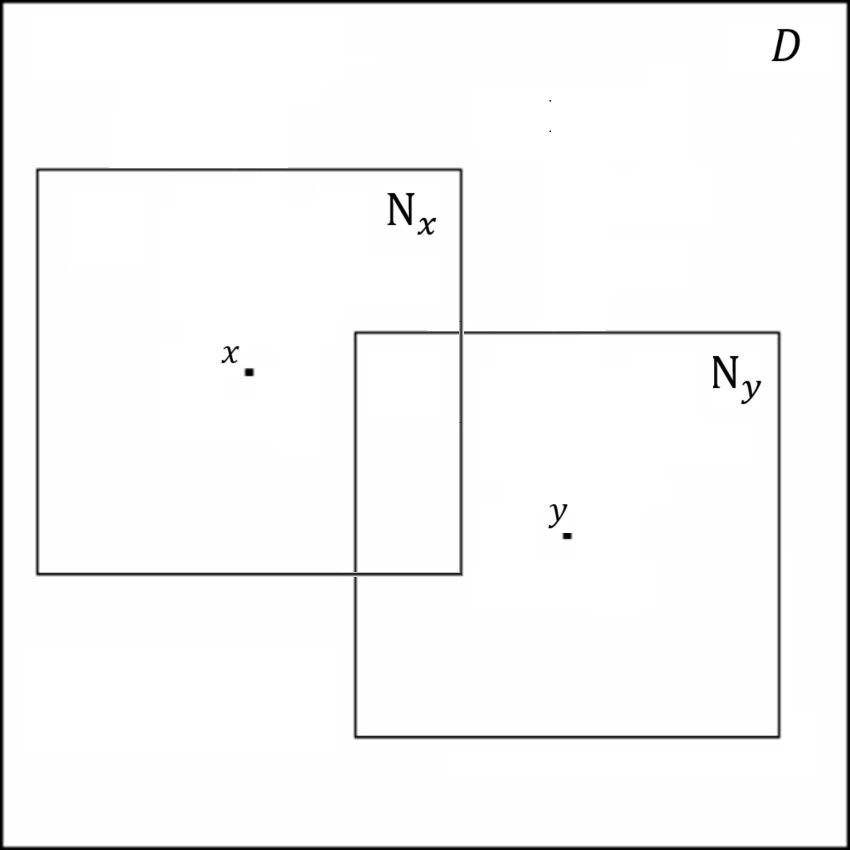
\includegraphics[scale=0.4]{rysunki/3_fig4.png}
	\caption{Przykładowe okna ${\boldsymbol{\mathrm{N}}}_{\boldsymbol{x}}\boldsymbol{,\ }{\boldsymbol{\mathrm{N}}}_{\boldsymbol{y}}$ utworzone dla pikseli $\boldsymbol{x},\boldsymbol{y}$.}
	\label{3_fig4}
\end{figure}
\par
Nielokalne operatory można przedstawić za pomocą zdyskretyzowanych równań:
\begin{equation}
{\mathrm{\nabla }}_{NLd}I|_{x,y}\triangleq \left(I_y-I_x\right)\sqrt{w_{x,y}}
\label{DNLGRAD}
\end{equation}
\begin{equation}
w_{x,y}={\mathrm{exp} \left\{-\sum_{y\in N_x,k\in N_y \\
}{{G_{\sigma}}_y \ast {\left|I_y-I_k\right|}^2}\right\}\ }
\label{DNLWEIGHT}
\end{equation}
\begin{equation}
{\left|\overrightarrow{p}\right|}_x\triangleq \sqrt{\sum_{y\in N_x \\ 
}{{\left(p_{x,y}\right)}^2}}
\label{DNLMAG}
\end{equation}
\begin{equation}
{\mathrm{\nabla }}_{NLd}\cdot \overrightarrow{p}\big|_x \triangleq \sum_{ 
y\in N_x \\ 
}{\left(p_{x,y}-p_{y,x}\right)}\sqrt{w_{x,y}}
\label{DNLDIV}
\end{equation}
\begin{equation}
{\mathrm{\Delta }}_{NL}{\overrightarrow{p}}\big|_x \triangleq \sum_{
y\in N_x \\ 
}{\left(I_y-I_x\right)}w_{x,y}
\label{DNLLAP}
\end{equation}
W szczególnym przypadku dla \eqref{NLDIVSMART} można zapisać:
\begin{equation}
{\mathrm{\nabla }}_{NLd}\cdot \overrightarrow{p}\big|_x \triangleq \sum_{ 
y\in N_x \\ 
}{2p_{x,y}}\sqrt{w_{x,y}}
\label{DNLDIVSMART}
\end{equation}
Warto zauważyć, iż indeksy $x,y$ wskazują na konkretny piksel w obrazie. Lokalizacji w przestrzeni $2D$ dokonuje się przez znajomość par: $x=(i_x,j_x)$ oraz $y=(i_y,j_y)$.
\par 
Nielokalny model wahania funkcji oznaczany $NLTV$ (non-local total variation) definiowany dla obrazów w odcieniach szarości przyjmuje następująca postać:
\begin{equation}
{\mathop{\mathrm{min}}_{u} \left\{E\left(u\right)=\ \int_D{\left|{\mathrm{\nabla }}_{NL}u(x)\right|}dx+\frac{1}{2}\int_D{\chi{\left(u-I^0\right)}^2}dx\ \right\}\ }
\label{NLTVGRAY}
\end{equation}
gdzie $I^0$ stanowi oryginalny obraz wejściowy, natomiast $u\left(x\right):D\mathrm{\longrightarrow }\mathrm{R}$ obraz wynikowy, będący obrazem wmalowanym, bądź w przypadku pierwotnych założeń obrazem z usuniętym szumem. W przypadku zagadnienia wmalowywania zmienna ${\chi }$ to funkcja definiowana na podstawie maski obrazu przyjmująca następujące wartości:
\begin{equation}
\chi \left(x\right)=\left\{ \begin{array}{c}
0\ x \in \Omega \\ 
\ \ \ \ \ 1\ x \in D/ \Omega \end{array}
\right\}
\label{maskFunction}
\end{equation}
Tak zdefiniowany model można przekształcić wykorzystując operację podziału Bregman’a. Podział stosuje się w celu poprawienia wydajności obliczeniowej w przypadku dyskretnej implementacji problemu minimalizacji energii. Wprowadzenie pomocniczej zmiennej $\overrightarrow{v}=v\left(x,y\right):\ \mathrm{\Omega }\mathrm{\ }x\ \mathrm{\Omega }\longrightarrow R$ i parametru Bregman’a $\overrightarrow{b}=\overrightarrow{b}\left(x,y\right):\ \mathrm{\Omega }\mathrm{\ }x\ \mathrm{\Omega }\longrightarrow R$ pozwala przekształcić problem minimalizacji powyższej energii do następującej postaci iteracyjnej:
\begin{align}
\begin{aligned}
\left(u^{k+1},{\overrightarrow{v}}^{k+1}\right) &= arg\ \mathop{\mathrm{min}}_{u,\overrightarrow{v}} E\left(u,\overrightarrow{v}\right)=\\ 
&= \biggl\{arg\ \mathop{\mathrm{min}}_{u,\overrightarrow{v}}
\int_D{|\overrightarrow{v}|\left(x\right)}dx+\frac{1}{2}\int_D{{\chi }{\left(u-I^0\right)}^2}dx+\\
&+  \frac{\mathrm{\Theta }}{2}\int_D{{\left|\overrightarrow{v}-{\mathrm{\nabla }}_{NL}u-{\overrightarrow{b}}^{k+1}\right|}^2(x)}dx\ \biggr\}
\end{aligned}
\label{NLTVGRAYMINPROB}
\end{align}
\begin{align}
{\overrightarrow{b}}^{k+1}={\overrightarrow{b}}^k+{\mathrm{\nabla }}_{NL}u^k-{\overrightarrow{v}}^k, {\overrightarrow{b}}^0={\overrightarrow{v}}^0=0
\label{BREGMANVARIABLE}
\end{align}
gdzie $\Theta$ stanowi wcześniej definiowany parametr algorytmu. Stosując podstawowe równanie rachunku wariacyjnego postaci równania Eulera-Lagrange’a, metodę przedstawioną w \cite{tai2011fast} oraz schemat iteracyjny Gauss’a-Seidel’a powyższe równania można sprowadzić do problemu iteracyjnego rozwiązania poniższych zależności:
\begin{align}
\chi \left(u-I^0\right)+\mathrm{\Theta }{\mathrm{\nabla }}_{NL}\cdot \left({\overrightarrow{v}}^k-{\mathrm{\nabla }}_{NL}u-{\overrightarrow{b}}^{k+1}\right)=0
\label{ELNLTV1}
\end{align}
\begin{align}
{\overrightarrow{v}}^{k+1}\mathrm{=}{\mathrm{max} \left(\left|{\mathrm{\nabla }}_{NL}u^{k+1}+{\overrightarrow{v}}^{k+1}\right|-\frac{1}{\mathrm{\Theta }},0\right)\cdot\frac{{\mathrm{\nabla }}_{NL}u^{k+1}+{\overrightarrow{b}}^{k+1}}{\left|{\mathrm{\nabla }}_{NL}u^{k+1}+{\overrightarrow{b}}^{k+1}\right|}\ }
\label{ELNLTV2}
\end{align}
Zależności te można stosować do obrazów w odcieniach szarości, bądź obrazów kolorowych traktując każdą z poszczególnych warstw osobnym algorytmem iteracyjnym. Zgodnie z \cite{duan2015fast} takie rozwiązanie prowadzi do niezachowania odpowiedniego kontrastu odrestaurowanej części obrazu i niezachowania krawędzi.
\par
W celu uzależnienia od siebie wszystkich warstw obrazu autorzy w \cite{duan2015fast} proponują zastosowanie funkcjonału MTV przedstawionego w \cite{yang2009fast}, funkcjonału $CTV$ przedstawionego w \cite{blomgren1998color}, bądź model Mumford-Shah’a dokładnie opisanego w \cite{jung2011nonlocal}. Ze względu na wydajniejszą implementację oraz najlepsze wyniki uzyskiwane w przypadku modelu $CTV$ został on wybrany do badań w niniejszej pracy. Wykorzystując wspomniany funkcjonał energia przyjmuje postać:
\begin{align}
{\mathop{\mathrm{min}}_{u} \left\{E\left(u\right)=\sqrt{\sum^m_{i=1}{{\left(\int_D{\left|{\mathrm{\nabla }}_{NL}u(x)\right|}dx\right)}^2}}+\frac{1}{2}\sum^m_{i=1}{\int_D{\chi{\left(u_i-I^0_i\right)}^2}dx}\ \right\}\ }
\label{ENLCTV}
\end{align}
gdzie $m$ odpowiada ilości warstw tworzących kolorowy obraz. Zastosowanie równania rachunku wariacyjnego postaci Eulera-Lagrange’a w swoim rozwiązaniu prowadzi do konieczności obliczenia nielokalnej krzywizny krzywej, będącej w przypadku dyskretyzacji rozwiązania znacznie obciążającą obliczeniowo operacją. W tym celu, podobnie jak w przypadku poprzedniego modelu $NLTV$ zastosowany zostanie heurystyczny algorytm podziału Bregman’a. Analogicznie wprowadzone zostają zmienne $\overrightarrow{v}=\left({\overrightarrow{v}}_1,{\overrightarrow{v}}_2,\ \dots ,\ \ {\overrightarrow{v}}_m\right)$ oraz $\overrightarrow{b}=\left({\overrightarrow{b}}_1,{\overrightarrow{b}}_2,\ \dots ,\ \ {\overrightarrow{b}}_m\right)$. Wtedy przytoczona energia przyjmuje iteracyjną postać: 
\begin{align}
\begin{aligned}
\mathop{\mathrm{min}}_{u}E\left(u\right) &= \mathop{\mathrm{min}}_{u}\Biggl\{\sqrt{\sum^m_{i=1}{{\left(\int_D{\left|\overrightarrow{v_i}\right|(x)}dx\right)}^2}}+\\ 
&+\frac{1}{2}\sum^m_{i=1}{\int_D{ \chi {\left(u_i-I^0_i\right)}^2}dx} 
+\frac{\theta }{2}\sum^m_{i=1}{\int_D{{\left|\overrightarrow{v_i}-{\mathrm{\nabla }}_{NL}u_i- {\overrightarrow{b_i}}^{k+1}\right|}^2\left(x\right)}dx}\Biggr\}
\end{aligned}
\label{ENLCTV1}
\end{align}
\begin{align}
{\overrightarrow{b_i}}^{k+1}={\overrightarrow{b_i}}^k+{\mathrm{\nabla }}_{NL}u^k_i-{\overrightarrow{v_i}}^k,\ {{\overrightarrow{b}}_i}^0={\overrightarrow{v_i}}^0=0
\label{ENLCTV2}
\end{align}
Przyjmując naprzemienną strategię minimalizacji energii można uzyskać równania Eulera-Lagrange’a wyznaczone oddzielnie względem zmiennych $u$ oraz $v$:
\begin{align}
\chi \left(u_i-I^0_i\right)+\mathrm{\Theta }{\mathrm{\nabla }}_{NL}\cdot \left({\overrightarrow{v_i}}^k-{\mathrm{\nabla }}_{NL}u_i-{{\overrightarrow{b}}_i}^{k+1}\right)=0
\label{ELNLCTV1}
\end{align}
\begin{align}
\mathrm{\Theta }\left(\overrightarrow{v_i}\mathrm{-}{\mathrm{\nabla }}_{NL}u^{k+1}_i\mathrm{-}{{\overrightarrow{b}}_i}^{k+1}\right)\mathrm{+}\frac{\int_D{\left|\overrightarrow{v_i}\right|(x)}dx}{\sqrt{\sum^m_{i=1}{{\left(\int_D{\left|\overrightarrow{v_i}\right|(x)}dx\right)}^2}\ }}\frac{\overrightarrow{v_i}}{\left|\overrightarrow{v_i}\right|(x)}\mathrm{=0}
\label{ELNLCTV2}
\end{align}
W celu przedstawienia dyskretnej formy równań \eqref{ELNLCTV1} i  \eqref{ELNLCTV2} i \eqref{ELNLCTV2} wygodnym będzie zapis dla konkretnego piksela $z\in D$ w obrazie. W przypadku \eqref{ELNLCTV1}: 
\begin{align}
\chi_z \left[u_{i_z}-{I^0_i}_z\right]+\mathrm{\Theta}{\mathrm{\nabla}}_{NL}\cdot \left({{\overrightarrow{v_i}}^k}_z-{{\mathrm{\nabla}}_{NL}u_i}\big|_z-{{{\overrightarrow{b}}_i}^{k+1}}_z\right)=0
\label{DELNLCTV1}
\end{align}
Korzystając z dyskretnych postaci równań \eqref{NLGRAD}, \eqref{NLWEIGHT}, \eqref{NLPRODUCT} i \eqref{NLDIV} równanie \eqref{ELNLCTV1} można przedstawić w postaci:
\begin{align}
\begin{aligned}
{u^{k+1}_i}_{z} &= \frac{1}{\chi_z+2\mathrm{\Theta} \sum\limits_{y\in N_i} w_{i_{z,y}}} \Biggl[2\mathrm{\Theta }\sum_{y\in N_i} {{{u^k_i}_y w_i}_{z,y}}+\\
&+ \chi_z \ {I^0_i}_z -\\
&-\mathrm{\Theta} \Biggl[\sum_{y\in N_z} \left({ v^k_i}_{z,y} - { v^k_i}_{z,y} - { v^k_i}_{z,y} + { v^k_i}_{z,y}\right) \sqrt{{w_i}_{z,y}} \Biggr]
\end{aligned}
\label{uNLCTV}
\end{align}
W przypadku równania \eqref{ELNLCTV1} Eulera-Lagrange’a należy przekształcić je względem zmiennej $\overrightarrow{v}$:
\begin{align}
\begin{aligned}
{\overrightarrow{v_i}}^{k+1} &= \mathrm{max} \left(\left|{\mathrm{\nabla }}_{NL}u^{k+1}_i+{\overrightarrow{b_i}}^{k+1}\right|-\frac{\int_D{\left|\overrightarrow{v_i}\right|(x)}dx}{\mathrm{\Theta }\sqrt{\sum^m_{i=1}{{\left(\int_D{\left|{\overrightarrow{v_i}}^k\right|(x)}dx\right)}^2}\ }},0\right) \\ 
&\cdot \frac{{\mathrm{\nabla }}_{NL}u^{k+1}_i+{{\overrightarrow{b}}_i}^{k+1}}{\left|{\mathrm{\nabla }}_{NL}u^{k+1}_i+{\overrightarrow{b_i}}^{k+1}\right|}\ 
\label{DELNLCTV2}
\end{aligned}
\end{align}
Podobnie, korzystając z dyskretnych form \eqref{NLGRAD}, \eqref{NLWEIGHT}, \eqref{FROBENIUS}, \eqref{NLPRODUCT} i \eqref{NLDIV} równanie \eqref{DELNLCTV2} można przedstawić w postaci:
\begin{align}
{{\overrightarrow{v_i}}^{k+1}}_z \cong {\mathrm{max} \left({\left|A^{k+1}_i\right|}_z-\frac{B^k_i}{\mathrm{\Theta }\sqrt{\sum^m_{i=1}{{\left(B^k_i\right)}^2}\ }},0\right)\frac{{A^{k+1}_i}_z}{{\left|A^{k+1}_i\right|}_z}\ }
\label{VNLCTVITER}
\end{align}
gdzie:
\begin{align}
{A^{k+1}_i}_z=\left({u^{k+1}_i}_y-{u^{k+1}_i}_z\right)\sqrt{w_{i_{z,y}}}+{b^{k+1}_i}_{z,y}
\end{align} 
\begin{align}
{\left|A^{k+1}_i\right|}_z=\sqrt{\sum_y{{\left[\left({u^{k+1}_i}_y-{u^{k+1}_i}_z\right)\sqrt{{w_i}_{z,y}}+{b^{k+1}_i}_{z,y}\right]}^2}\ }
\end{align}
\begin{align}
B^k_i=\sum_z{\sqrt{\sum_y{{{v^k_i}^2}_{z,y}}}}
\end{align}
Warto przypomnieć, iż w przytoczonych wzorach $y$ odpowiada pikselom znajdującym się oknie poszukiwania ${\mathrm{N}}_z$ scentrowanym względem piksela $z$, natomiast $i$ odpowiada $i$-tej warstwie spośród warstw tworzących obraz kolorowy. Autorzy w \cite{jung2011nonlocal} proponują zmodyfikowany sposób wyznaczania wagi uwzględniający kształt maski w obrazie:
\begin{align}
w\left(x,y\right)\triangleq {\mathrm{exp} \left\{-\frac{G_{\sigma }*{\chi }_R\left(x+\ \cdot \right){\left|I\left(x+\ \cdot \right)-I\left(y+\ \cdot \right)\right|}^2}{r^2}\right\}\ }
\label{NLWEIGHTMASK}
\end{align}
gdzie:
\begin{equation}
{\chi }\left(x\right)=\left\{ \begin{array}{c}
0 \ x \in  \mathrm{\Omega} \\ 
\ \ \ \ \ 1 \ x \in  D/\mathrm{\Omega} \end{array}
\right\}
\end{equation}
Podsumowując algorytm wmalowywania w oparciu o model $NLCTV$ z algorytmem podziału Bregman’a można przedstawić w następujących krokach:
\begin{enumerate}
\item  
Inicjalizacja zmiennych $k=0,\ \overrightarrow{b^0_i}=0,\ \overrightarrow{v^0_i}=0,\ u^0_i=f^0_i$ 
\item  
Wyznaczenie wagi $w^2_i$ zgodnie z \eqref{NLWEIGHTMASK} dla całego obszaru obrazu $D$
\item  
Powtarzanie do spełnienia kryterium końcowego:
\begin{itemize}
%\addtolength{\itemindent}{1cm}
\item
\noindent Wyznaczenie ${\overrightarrow{b}}^{k+1}={\overrightarrow{b}}^k+{\mathrm{\nabla }}_{NL}u^k-{\overrightarrow{v}}^k$
\item
\noindent Wyznaczenie $u^{k+1}$ na podstawie \eqref{DELNLCTV1} dla każdego piksela $z$
\item
\noindent Wyznaczenie $v^{k+1}$ na podstawie \eqref{VNLCTVITER} dla każdego piksela $z$
\end{itemize}
\item  
Aktualizacja wagi $w^2_i$ w obszarze $\mathrm{\Omega }$
\end{enumerate}
Kryterium definiującym zakończenie algorytmu może być uzyskanie granicznej wartości różnicy wcześniej zdefiniowanej energii $\varepsilon$ pomiędzy wykonywanymi iteracjami:
\begin{equation}
\left|E^{k+1}-E^k\right|\le \varepsilon
\end{equation}
\section{Wariacyjny, nielokalny model wmalowywania}
Kolejną z rozważanych metod będzie metoda zaproponowana przez Fedorov'a, Facciolo i Arias'a w \cite{arias2011variational}. Autorzy publikacji proponują optymalizację energii $\mathcal{E}(\varphi(x), u(\Omega))$ zależnej:
\begin{itemize}
\item
od nieznanego obszaru obrazu $u(\Omega)$
\item
od mapy podobieństwa będącej funkcją przypisującą każdemu puntowi z nieznanego obszaru jego konkretnego odpowiednika z obszaru znajdującego się poza maską $\varphi(x)$
\end{itemize}
\begin{figure}[!h]
	\centering
	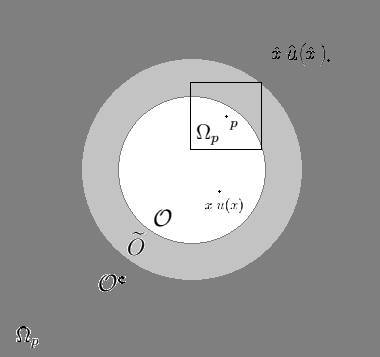
\includegraphics[scale=0.9]{rysunki/6_fig1}
	\caption{Określenie charakterystycznych obszarów obrazu.}
	\label{6_fig1}
\end{figure}
Oznaczmy funkcję $u(x)$ na zbiorze $\Omega$, dla której zachodzi $u:\Omega \rightarrow R$, gdzie $\Omega$ oznacza obszar do uzupełnienia.
Oznaczmy funkcję $\hat{u}(\hat{x})$ na zbiorze $D$, dla której zachodzi $\hat{u} : D \rightarrow R$, gdzie $D$ oznacza obszar oryginalnego obrazu nie podlegający modyfikacji.
Niech $\mathrm{N}_x$ i $\mathrm{N}_{\hat{x}}$ oznaczają podzbiory punktów obrazu scentrowane względem odpowiednio punktów $x$ i $\hat{x}$.
Wtedy zbiór $\widetilde{\Omega}$ definiuje się jako $\widetilde{\Omega} := \Omega + \sum {\mathrm{N}}_x$, gdzie $\sum {\mathrm{N}}_x$ to suma wszystkich podzbiorów utworzonych względem punktów $x \in \Omega$. Ostatecznie $D^c = D / \widetilde{\Omega}$.
Zgodnie z \cite{arias2011variational} przekształcenie $u(x)$ jest zarezerwowane dla obszaru maski (obszaru wmalowywanego), a $\hat{u}(\hat{x})$ odpowiada przekształceniu w niezmienianym obszarze obrazu $D$). 
Przekształcenie funkcji podobieństwa $\varphi(x)$ przedstawia \autoref{6_fig2}.
\begin{figure}[!h]
	\centering
	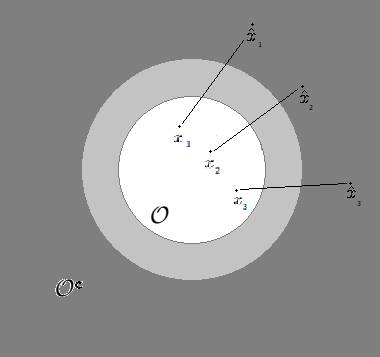
\includegraphics[scale=0.9]{rysunki/6_fig2}
	\caption{Funkcja podobieństwa $\varphi(x)$ : $\varphi(x_1)=\hat{x_1}, \varphi(x_2)=\hat{x_2}, \varphi(x_3)=\hat{x_3}$.}
	\label{6_fig2}
\end{figure}
Energię poddawaną minimalizacji można wyrazić zależnością:
\begin{align}
\begin{aligned}
\mathcal{E}(u,\varphi) = \int_{\mathcal{\widetilde{O}}}\int_{\Omega_p}\abs{u(x+h) - \hat{u}(\varphi(x)+h)}^2dhdx
\end{aligned}
\end{align}
Funkcja ta jest niewypukła i pozwala obliczyć jedynie lokalne minima. W pracy wykorzystano iteracyjny algorytm naprzemiennej minimalizacji polegający na wyznaczaniu w każdym kroku $u(x)$ względem stałej wartości $\varphi(x)$, a następnie $\varphi(x)$ względem stałej wartości $u(x)$.
\subsection{Wyznaczenia mapy podobieństwa.}
Proces minimalizacji funkcji przyjmując ustaloną wartości
\begin{equation}
u(x) = \text{const}
\end{equation}
można opisać zależnością:
\begin{align}
\begin{aligned}
\mathop{\operatorname{arg \ min}}_{t} \ \mathcal{E}\biggl( u(x+\cdot) - {\hat{u}}\bigl((x+t)+\cdot\bigr)\biggr),\operatorname{gdzie} \ \forall_t : x+t \in D^c
\label{minNNF}
\end{aligned}
\end{align}
Zmienna $t$ w tym zagadnieniu przyjmuje takie wartości ze zbioru wektorów przemieszczeń, których suma z danym wektorem położenia $x$ lokalizuje go w obszarze $D^c$. Wynikiem minimalizacji jest $\varphi$, która stanowi funkcję wyznaczającą najbliższego sąsiada punktu $x$ z przestrzeni $D^c$, $\varphi :\Omega \rightarrow D^c$. Warto zaznaczyć, że przez pojęcie najbliższego sąsiada punktu $x$ rozumiemy nie punkt znajdujący się najbliżej, ale ten piksel dla którego zgodnie z przyjętą normą uzyskuje się najniższą wartość z pośród wszystkich możliwych:
\begin{align}
\begin{aligned}
\big\| u(x + \cdot) - \hat{u}(\hat{x}+\cdot) \big\| 
\label{normNNF}
\end{aligned}
\end{align}
Norma ta może być wyznaczana zgodnie z zależnością \eqref{NLWEIGHT} bądź \eqref{FROBENIUS}. Autorzy w \cite{MathematicalModelsforNLTextureInpainting} proponują dodatkowe definicje norm, które zostaną opisane w dalszej części pracy. Najprostszy algorytm wyznaczania najbliższego sąsiada może osiągnąć złożoność do $O(N^3)$ i wymagać znacznych nakładów obliczeniowych. Autorzy w \cite{arias2011variational} proponują zastosowanie algorytmu PatchMatch dokładnie opisanego w \cite{barnes2009patchmatch}. Algorytm ten oparty jest na dwóch krokach. Niech punkt $x$ odpowiada współrzędnym $i, j$ obrazu, natomiast dla uproszczenia zapisu oznaczmy $u(x+\cdot)$ jako $p_u(i,j)$. Wtedy kroki można opisać następująco:
\begin{enumerate}
\item
Losowej inicjalizacji pikseli
\item
Ograniczonej wcześniej definiowaną liczbą iteracji powtarzanej czynności:
\begin{enumerate}[a)]
\item
propagacja: w przypadku parzystej iteracji dla sprawdzenia wszystkich pikseli $x$ z maski w kierunku rastrowym przedstawionym na \autoref{6_fig3}, czy 
wartość $\big\| p_u(i,j) - p_{\hat{u}}(\varphi(i+1,j)) \big\|$, bądź $\big\| p_{u}(i,j) - p_{\hat{u}}(\varphi(i,j+1)) \big\|$ nie jest mniejsza od obecnie wyznaczonej i w takim przypadku zmienić najbliższego sąsiada według formuły $\varphi(i,j) = \varphi(i+1,j)$, lub $\varphi(i,j) = \varphi(i,j+1)$, 
w przypadku nieparzystej iteracji należy sprawdzić dla wszystkich pikseli $x$ w kierunku odwrotnym do rastrowego przedstawionym na \autoref{6_fig3}, czy 
wartość $\big\| p_{u}(i,j) - p_{\hat{u}}(\varphi(i-1,j)) \big\|$ bądź $\big\| p_{u}(i,j) - p_{\hat{u}}(\varphi(i,j-1)) \big\|$ nie jest mniejsza od obecnie wyznaczonej i w takim przypadku trzeba zmienić najbliższego sąsiada według formuły $\varphi(i,j) = \varphi(i-1,j)$, lub $\varphi(i,j) = \varphi(i,j-1)$
\item
poszukiwanie w oknach: dla każdego punktu $(i,j)$ sprawdzane jest, czy w stopniowo pomniejszanych oknach centrowanych względem punktu $\varphi(i,j)$ istnieje losowy punkt $(i', j')$, dla którego zachodzi nierówność $\big\| p_{u}(i,j) - p_{\hat{u}}(i',j') \big\| < \big\| p_{u}(i,j) - p_{\hat{u}}(\varphi(i,j) \big\|$, jeśli tak to punkt ten jest podmieniany.
\end{enumerate}
\end{enumerate}
\begin{figure}[!h]
	\centering
	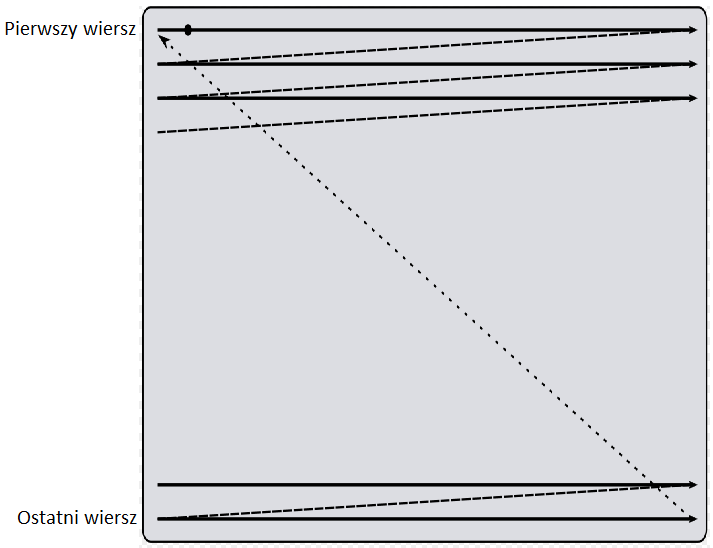
\includegraphics[scale=0.5]{rysunki/6_fig3}
	\caption{Funkcja podobieństwa $\varphi(\hat{x})$ : $x_1 = \varphi(\hat{x_1}), x_2 = \varphi(\hat{x_2}), x_3 = \varphi(\hat{x_3})$.}
	\label{6_fig3}
\end{figure}
Kroki algorytmu PatchMatch zostały przedstawione graficznie na \autoref{6_fig4}.
\begin{figure}[!h]
	\centering
	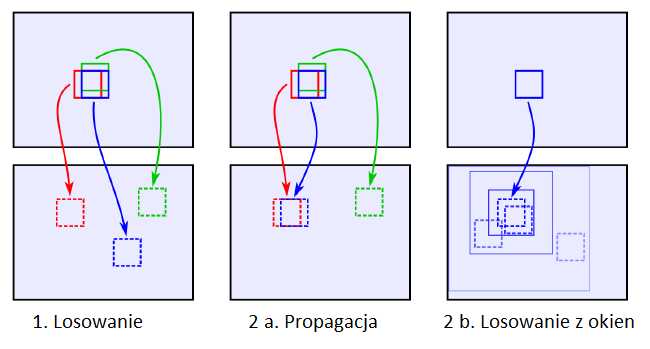
\includegraphics[scale=0.9]{rysunki/6_fig4}
	\caption{Algorytm PatchMatch. Źródło \cite{arias2011variational}.}
	\label{6_fig4}
\end{figure}
\subsection{Wyznaczenie wartości obrazu.}
Niech funkcja $e$  będzie przekształceniem $e: \mathrm{N}_x \rightarrow {\rm I\!R}^{+}$ której wartość reprezentuje sumę ważonych błędów pomiędzy dwoma fragmentami obrazu scentrowanymi względem punktów $x$ i $\hat{x}$, korzystając z wcześniej wprowadzonych oznaczeń:
\begin{align}
\begin{aligned}
e(x, \hat{x}) &= G_\sigma \ast \big\| u(x + \cdot) - u(\hat{x} + \cdot) \big\| = G_\sigma \ast \big\| p_{u}(x) - p_{\hat{u}}(\hat{x}) \big\| = \\ 
&= \int_{\mathrm{N}_x} G_\sigma(h) \big\| u(x+h) - \hat{u}(\hat{x} +h) \big\|dh
\label{minUs}
\end{aligned}
\end{align}
gdzie zmienna $G_{\sigma}$ została wprowadzona dla algorytmu $NLCTV$ i opisywana jest zależnością \eqref{oknoGaussowskie}. Autorzy w \cite{arias2011variational} proponują minimalizację następującej energii będącej akumulacją błędów pikseli:
\begin{align}
\begin{aligned}
E(u) &= \int_{\widetilde D}\int_{\mathrm{N}_x}G_\sigma(h)\cdot e \bigl( u(x+h) - \hat{u}(\varphi(x)+h\bigr)dhdx
\label{patchMatchEnergy}
\end{aligned}
\end{align} 
Niech $z := x+h$ i $\hat{z} := \hat{x}+h$. Wprowadzamy zależność:
\begin{align}
m(z,\hat{z}) = \int_{\mathrm{N}_x}G_\sigma(h)\chi_{z-h}\delta_{\varphi(z-h)}(\hat{z}-h)dh
\end{align}
gdzie:
\begin{enumerate}
\item
zmienna $\chi$ została już zdefiniowana w modelu $NLCTV$ \eqref{maskFunction} i przyjmuje wartość $1$ poza maską i wartość $0$ w masce.
\item
$\delta(p)$ określa pewność co do danego piksela wewnątrz maski i jest określone następującą zależnością:
\begin{align}
\delta(x)=(1-c_0)exp\bigg(\frac{-\mathrm{d}\bigl(x,\partial\Omega\bigr)}{t_c}\bigg) + c_0
\label{pewnoscVFI}
\end{align}
\end{enumerate}
przy czym wartość $t_c$ określa szybkość opadania funkcji wykładniczej, natomiast $c_0$ asymptotę, do której to funkcja zmierza. Odległość punktu od granicy maski określona jest zależnością $\frac{-\mathrm{d}(x,\partial\Omega)}{t_c}$ W zależności od zastosowanej normy \eqref{normNNF} rozwiązanie problemu minimalizacji energii uzyskuje różne postacie. Autorzy w \cite{arias2011variational} przedstawiają rozwiązanie dla następujących norm:
\begin{enumerate}
\item
Normy nielokalnej uśredniającej:
\begin{align}
\begin{aligned}
\big\| p_{u}(x) - p_{\hat{u}}(\hat{x}) \big\|^{2}_{g,2} = g \ast | u(x+\cdot) - \hat{u}(\hat{x}+\cdot) |^2
\label{nonLocalMeans}
\end{aligned}
\end{align}
\item
Normy nielokalnej medianowej:
\begin{align}
\begin{aligned}
\big\| p_{u}(x) - p_{\hat{u}}(\hat{x}) \big\|_{g,1} = g \ast | u(x+\cdot) - \hat{u}(\hat{x}+\cdot) |
\label{nonLocalMedians}
\end{aligned}
\end{align}
\item
Normy nielokalnej Poissona:
\begin{align}
\begin{aligned}
\big\| p_{u}(x) - p_{\hat{u}}(\hat{x}) \big\|_{P} &= \big\| p_{u}(x) - p_{\hat{u}}(\hat{x}) \big\|^{2}_{g,2} + \big\| p_{u}(x) - p_{\hat{u}}(\hat{x}) \big\|^{2}_{g,2,\nabla} \\
&= g \ast (\lambda | u(x+\cdot) - \hat{u}(\hat{x}+\cdot) | \\
&+ (1-\lambda)|\nabla u(x+\cdot) - \nabla \hat{u}(\hat{x}+\cdot)|
\label{nonLocalpoisson}
\end{aligned}
\end{align}
\end{enumerate}
Indeksy dolne $g, 1, 2, \nabla$ przy zapisach nielokalnych norm oznaczają odpowiednio: uwzględnienie zmiennej \eqref{oknoGaussowskie} w wyznaczaniu odległości, normę wektorową $\ell_{1}$, normę wektorową $\ell_{2}$, obliczanie dystansu na podstawie dywergencji rozmażanego pola. Stąd suma różnic pikseli w przypadku normy Poissona wymaga dodatkowo wyznaczenia dywergencji obrazu. Współczynnik $\lambda$ określa w jakim stopniu poszczególny z członów będzie miał wpływ na ostatecznie uzyskiwany wynik. Dla norm uzyskuje się odpowiednio rozwiązania w postaci:
\begin{enumerate}
\item
równanie:
\begin{align}
u(z) = \frac{1}{k(z)}\int_{\widetilde O^c}m(z,\hat{z})\hat{u}(\hat{z})d\hat{z}
\end{align}
gdzie
\begin{align}
k(z) := \int_{\widetilde D}^c m(z,\hat{z})d\hat{z}
\end{align}
\item
równanie Eulera:
\begin{align}
[\delta_{u}\mathcal{E}(u)](z) = \int_{D^c}sign[u(z)-\hat{u}(\hat{z})]m(z,\hat{z})d\hat{z} \ni \Omega 
\end{align}
\item
równania Eulera rozwiązane względem zmiennej $u$:
\begin{align}
\begin{aligned}
\begin{cases}
\nabla \cdot [k(z)\nabla u(z)] - \frac{\lambda}{1-\lambda}]k(z)u(z) = \\ 
\ \ \ \ \ = \nabla \cdot [k(z)\nabla v(z)] - \frac{\lambda}{1-\lambda}]k(z)f(z) , & z \in \Omega \\
u(z)=\hat{u}(z) , & z \in \partial \Omega \setminus \partial \mathrm{N} \\
\nabla u(z) \cdot n_{\mathrm{N}}(z) = 0 , & z \in \partial \Omega \cap \partial \mathrm{N}
\end{cases}
\end{aligned}
\end{align}
gdzie:
\begin{align}
v(z) := \frac{1}{k(z)}\int_{D^c}m(z,\hat{z})\nabla\hat{u}(\hat{z})d\hat{z}
\end{align}
\begin{align}
f(z) := \frac{1}{k(z)}\int_{D^c}m(z,\hat{z})\hat{u}(\hat{z})d\hat{z}
\end{align}
\end{enumerate}
Dokładne wyprowadzenia zależności można znaleść w \cite{arias2011variational}.
\subsection{Wielostopniowy schemat wypełniania.}
W wielu metodach wypełniania braków w obrazie stosowany jest algorytm wielostopniowy, przykładem mogą być \cite{kawai2009image}, \cite{komodakis2007image} bądź \cite{wexler2007space}. Algorytm ten polega na utworzeniu serii mniejszych przeskalowanych obrazów, następnie wypełnianiu ich począwszy od najmniejszego z warunkami początkowymi uzyskanymi poprzez przeskalowanie do większego obrazu wcześniej wyznaczonych wartości w masce. W przypadku najmniejszego obrazu z serii warunkami początkowymi mogą być:
\begin{itemize}
\item
losowo wyznaczone wartości obrazu pobierane z obszaru $D^c$
\item
rozwiązanie równania Poisson'a \eqref{Poisson2D}, dokładnie przedstawione w \autoref{chap:navierstokes}, metodą SOR ( z ang. succesive over relaxation method) zgodnie z zależnością \eqref{DiscreteSOR}.
\end{itemize}
Przeskalowywanie w obie strony musi odbywać się w sposób nie zniekształcający głównych struktur, obiektów i tekstur obrazu. W tym celu autorzy \cite{arias2011variational} proponują model piramidy Gaussa.\\
W celach wmalowywania tworzone są dwie oddzielne piramidy wyznaczające maski obrazu i same obrazy. Niech $S$ oznacza liczbę poziomów piramidy, a rozmiar oryginalnego obrazu jest oznaczany przez $s=0$. Niech rozmiar najmniejszego stopnia określa $A_{S-1}$, natomiast rozmiar oryginalnego obrazu $A_{0}$. Wtedy współczynnik próbkowania do tworzenia coraz mniejszych obrazów wynosi:
\begin{align}
r := \left(\frac{A_0}{A_{s-1}}\right)^\frac{1}{s-1}
\end{align}
W rezultacie aby uzyskać mniejszy obraz musi zachodzić $r \geq 1$. Parametr $\sigma$ tworzonego filtru Gauss'a wyznaczany jest z zależności $\sigma(r)=0.62\sqrt[2]{r^2-1}$. Rozmiar okna Gauss'a wykorzystywanego do filtrowania można przyjąć jako wartość stałą zdefiniowana z góry. Niech indeks górny s odnosi się do zmiennych oraz do obszarów w zakresie rozważanego poziomu piramidy. W przypadku tworzenia kolejnych masek wykorzystywane jest próbkowanie w dół z ograniczeniem w postaci zależności między funkcjami charakterystycznymi wmalowywanych obszarów $\Omega^s$ i $\Omega^{s+1}$:
\begin{align}
\chi_{\Omega^{s+1}}=(\downarrow_r G_{\sigma(r)}\ast\chi_{\Omega^s})> T_{0}.
\end{align}
Autorzy w \cite{arias2011variational} proponują wartość $T_0=0.4$. Niech $f$ stanowi wynik próbkowania w dół z filtrem Gauss'a. Zapis ten oznacza, iż w przypadku gdy $f(x)>0.4$ punkt w przekształceniu traktowany jest jako punkt źródłowy obrazu nie wymagający wmalowania. W przypadku obrazu wykorzystywana jest zależność
\begin{align}
u^{s+1}(x)= \downarrow_r \frac{G \ast \chi_{(D^s)}^c u^s(x)}{G \ast \chi_{{(D^s)}^c}(x)}
\end{align}
Powyższe równanie przedstawia ograniczenie w postaci nieuwzględniania wartości znajdujących się w obszarze $D^c$. Obraz w pierwszym kroku zostaje przemnożony przez maskę przedstawiającą źródłową część obrazu, następnie dokonywana jest operacja splotu obrazu z utworzonym filtrem Gauss'a normalizowany członem $G \ast \chi_{(D^s)^c}(x)$. W przypadku próbkowania w górę, wyznaczane są dwie piramidy: obraz w ograniczeniu do obszaru wmalowanego na poprzednim poziomie oraz pomocnicza funkcja przedstawiająca mapę podobieństwa. Do tego został wykorzystany algorytm dokładnie przedstawiony w \cite{wexler2007space} i opisany w \cite{arias2011variational}.
\subsection{Podsumowanie algorytmu}
Łącząc opisane powyżej operacje dokonywane na obrazie algorytm wypełniania można przedstawić w następujących krokach:
\begin{enumerate}
\item
Ustawienie argumentów algorytmu: obraz $u^{0}$, maska obrazu $\chi$, liczba poziomów piramidy $S$, rozmiar najmniejszego obrazu $A_{S-1}$, ilość iteracji minimalizacji energii $K$
\item
Wyznaczenie piramidy maski stanowiącej zbiór: $\{\chi^s\}_{s=0,...,S-1}$ \\
Wyznaczenie piramidy obrazu stanowiącej zbiór: $\{u^s\}_{s=0,...,S-1}$
\item
Inicjalizacja obrazu $u^{S-1}$ w obszarze $\Omega$ \\
Wyznaczenie mapy podobieństwa $\varphi^{S-1}$ na podstawie $u^{S-1}$
\item
Wykonanie dla każdego z poziomów piramidy $s$ począwszy od $S-2$ do $0$:
\begin{enumerate}[a)]
\item
Przeskalowanie mapy podobieństwa z zastosowaniem algorytmu interpolacji najbliższego sąsiada $\varphi^s=r \cdot (\uparrow_r \varphi^{s+1})$
\item
Wyznaczenie przeskalowanego obrazu $u^s_0=r \cdot (\uparrow_r u^{s+1})$ i przepisanie wartości $u^s(\Omega)=u^s_0(\Omega)$ w celu inicjalizacji
\item
Powtarzanie $I$-tą ilość razy z wykorzystaniem odpowiedniej normy \eqref{normNNF}
\begin{itemize}
\item
przeprowadzenie \eqref{minNNF} w celu wyznaczenia $\varphi^s$
\item
przeprowadzenie \eqref{minUs} w celu wyznaczenia $u^s$
\end{itemize}  
\end{enumerate}
\end{enumerate}
Wynikiem powyższej instrukcji jest zbiór obrazów $\{u^s\}$ oraz map podobieństwa $\{\varphi^s\}$, gdzie $s \in {0,...,S-1}$
\chapter{Uzupełnianie kawałkami obrazu.}
\section{Metoda Criminisi.}
Kolejną grupą algorytmów rozważanych w niniejszej pracy jest grupa opierająca się na wypełnianiu brakujących obszarów w obrazie fragmentami pochodzącymi z ich otoczenia. W odróżnieniu od różnych algorytmów bazujących na równaniach różniczkowych metoda ta nie bazuje na metodzie dyfuzji. Pierwszy raz zaproponowana została w \cite{efros1999texture}, a jej podstawowy krok opiera się na schemacie przedstawionym na \autoref{4_fig1}.
\begin{figure}[!h]
	\centering
	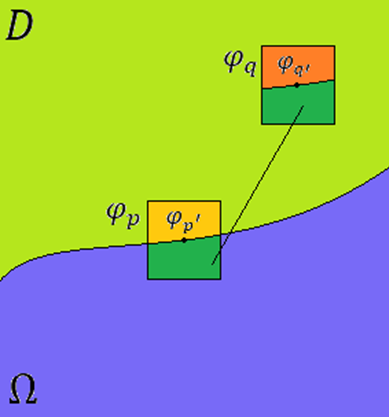
\includegraphics[scale=0.5]{rysunki/4_fig1}
	\caption{Schemat wmalowywania obrazu.}
	\label{4_fig1}
\end{figure}
Podobnie jak w poprzednich działach niech zbiór $D$ oznaczony kolorem jasnozielonym określa znane punkty obrazu, natomiast $\Omega$ oznaczony kolorem fioletowym określa obszar do odrestaurowania.
Niech oznaczenie $\hat{u}(\hat{x})$ stanowi funkcję na obszarze $D^c$, $\hat{x}  \in D^c$ (\autoref{6_fig1}).
Niech $q_{\hat{x}}$ stanowi podzbiór wartości punktów obrazu scentrowanych względem piksela $\hat{x}$ o zdefiniowanym z góry promieniu otoczenia.
Dla $q_{\hat{x}}$ zachodzi $\forall p \in q_{\hat{x}} : \chi(p) \neq 0$, gdzie $\chi$ odpowiada funkcji maski \eqref{maskFunction}.
Niech $p_{x}$ stanowi podzbiór punktów tworzących fragment obrazu o rozmiarze równym rozmiarowi $q_{\hat{x}}$, scentrowanych względem piksela $x$, gdzie $x \in \partial \Omega$.
Zdefiniujmy dwa podzbiory punktów:
\begin{align}
\begin{aligned}
p_{x} = s_x + i_x
\end{aligned}
\end{align}
gdzie $\forall p \in s_x : \chi(p) = 1$ i $s_x$ oznacza wypełnioną część fragmentu oraz $\forall p \in i : \chi(p) = 0$ czyli $i_x$ jako brakująca część fragmentu obrazu.  
Oznaczmy odpowiednio zbiory $\hat{s}_{\hat{x}}$ i $\hat{i}_{\hat{x}}$ będące przekształceniem zbiorów $s_x$ i $i_x$ o wektor $\overrightarrow{|x \hat{x}|}$:
\begin{align}
\begin{aligned}
q_{\hat{x}} = \hat{s}_{\hat{x}} + \hat{i}_{\hat{x}}
\end{aligned}
\end{align}
Podstawową operacją wmalowywania metodą propagacji tekstury obrazu jest znalezienie pary
 najbardziej podobnych do siebie fragmentów $\left\langle p_{x}, q_{\hat{x}} \right\rangle $ oraz zgodnie z \autoref{4_fig1} przepisanie wartości odpowiednich pikseli z wyznaczonego zbioru $\hat{i}_{\hat{x}}$ do odpowiadających im pikseli w zbiorze $i_x$ oznaczonych kolorem ciemnozielonym. Zapisując to w sposób formalny szukamy:
\begin{align}
\mathrm{arg} \mathop{\mathrm{min}}_{\hat{y} \in D^c} \big\| u(p_x) - \hat{u} (q_{\hat{y}} ) \big\| 
\label{FROBDIST}
\end{align}
Najprościej odległość pomiędzy dwoma fragmentami $d\left( u(p_x), \hat{u} (q_{\hat{y}}) \right)$ może być definiowana jako suma kwadratów różnic odpowiadających sobie pikseli ze zbiorów $s_x$ i ${\hat{s}}_{\hat{y}}$:
\begin{align}
d\left( u(s_x) - \hat{u}( \hat{s}_{\hat{y}} )\right)= \sum_{z \in s_x} \left( \hat{u}(z + \overrightarrow{|x \hat{x}|}) - u(z) \right)^2
\label{FROBENIUS2} 
\end{align}
W celu odrestaurowania obrazu powyższy schemat powtarzany jest aż do momentu wypełnienia całego obszaru $\mathrm{\Omega }$.
Metoda wmalowywania pierwszy raz przedstawiona w  \cite{efros1999texture} nie zakłada żadnego priorytetu ani kolejności wypełniania braków ustalanej na podstawie otoczenia maski. Tak przeprowadzana synteza obrazu pomimo wyznaczenia dla danego piksela trafnego dopasowania względem zdefiniowanej odległości może prowadzić do niespójności obrazu, przykład na \autoref{5_fig2}
\begin{figure}[!h]
	\centering
	\includegraphics[scale=0.3]{rysunki/5_fig2}
	\caption{Niespójność obrazu przy najlepszym dopasowaniu. $A$ - odrestaurowywany obraz, $B$ - wynik algorytmu, $C$ - oczekiwany wynik.}
	\label{5_fig2} 
\end{figure}
\begin{figure}[!h]
	\centering
	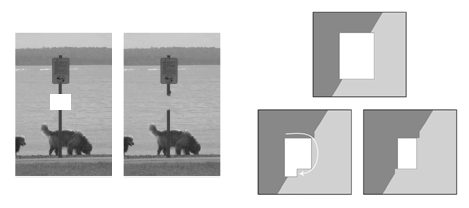
\includegraphics[scale=1]{rysunki/4_fig2}
	\caption{Wpływ prostego schematu wypełniania braków na wynikową teksturę obrazu. Źródło \cite{criminisi2004region}.}
	\label{4_fig2} 
\end{figure}
W 2004 roku Criminisi w \cite{criminisi2004region} skorzystał z koncepcji próbkowania fragmentów obrazu proponując nowe podejście do wyznaczania kolejności ich wmalowywania.  Kolejność wypełniania wyznaczana jest na podstawie izolinii poziomu jasności obrazu. W każdej iteracji algorytmu dla pikseli sąsiadujących z maską wyznaczane są wartości priorytetu wypełniania. Następnie wypełnienie odbywa się dla piksela o największym priorytecie. Dzięki nowemu podejściu izolinie będące granicami struktur obrazu są kontynuowane w miejscach odrestaurowywanych.
Algorytm przedstawiony w \cite{criminisi2004region} opiera się na powtarzaniu trzech głównych kroków w każdej iteracji wykonywanej do momentu wypełnienia wszystkich pikseli ze zbioru $\mathrm{\Omega }$.
Każda kolejna iteracja prowadzi do przesunięcia granicy maski $\partial \Omega$ w jej głąb. Pierwsze dwa kroki w pojedynczej iteracji służą do wyznaczenia priorytetu $P\left(x\right)$ dla każdego piksela obrazu znajdującego się na granicy maski $x \in \partial \Omega$, natomiast trzeci krok służy znalezieniu najlepszego punktu dopasowania $\hat{x}$.
Priorytet $P \left( x \right)$ każdego piksela $x$ wyznaczany jest z zależności:
\begin{align}
P\left( x \right)=C_t(x)\cdot D_t(x)
\label{PRIORITY}
\end{align}
Pierwszy krok w każdej wykonywanej iteracji związany jest z obliczeniem wartości funkcji $C_t(x)$ definiowanej (z ang. $C_t$ - confidence term, $D_t$ - data term):
\begin{align}
C_t\left( x \right)=\ \frac{\sum_{z \in s_x} {C(z)}}{\left|p_x\right|}
\label{confidenceTerm}
\end{align}
gdzie $C(x)$ to funkcja przypisująca wszystkim pikselom z obrazu poziom wiarygodności odwzorowania oryginalnego obrazu, $\left| p_x\right |$ - liczba pikseli w analizowanym fragmencie - rozmiar rozważanego okna. 
Podczas inicjalizacji funkcja $C$ dla każdego piksela stanowiącego oryginalny obraz przyjmuje wartość $1$, natomiast dla punktów maski przyjmuje wartość $0$. Matematycznie ${\forall }_{z \in D}\ C\left( z \right)=1$  i analogicznie ${\forall }_{z\in \mathrm{\Omega }}\ C\left( z \right)=0$. Wraz z wyznaczaniem kolejnych wartości pikseli należących do obszaru maski funkcja $C$ jest aktualizowana, a zerowe wartości są odpowiednio przeliczane. Funkcja $C_t(x)$ jest sumą wartości $C_t(y)$ wszystkich pikseli z analizowanego fragmentu obrazu $y \in s_x$ scentrowanego względem piksela $x$, które znajdują się w przestrzeni wyznaczonego już obrazu, podzieloną przez ilość pikseli w danym skrawku. Funkcję tą interpretuje się jako czynnik wymuszający koncentryczne, czyli postępujące wypełnianie wzdłuż granicy maski nieznanych punktów zgodnie z pierwotnym założeniem w \cite{efros1999texture}. Wynika to z pierwszeństwa jakie wprowadza funkcja $C_t$ przypisując w każdej iteracji coraz niższe wartości kolejnym wypełnianym pikselom. W ten sposób pierwszeństwo wypełniania uzyskują wycinki obrazu zawierające większą liczbę pikseli wypełnionych w poprzednich iteracjach, bądź zawierających oryginalne części obrazu. Mniejszą wartość $C$ w każdym kroku interpretuje się jako mniejszą pewność co do wyznaczonych wartości koloru w obrazie.
Drugi krok w każdej wykonywanej iteracji związany jest z obliczeniem wartości funkcji $D_t(x)$ definiowanej jako:
\begin{align}
D_t(x)= \frac{\left|\nabla^{\bot}u_x \cdot n_x\right|}{\alpha }
\label{DataTerm}
\end{align}
gdzie człon ${\mathrm{\nabla }}^{\bot }u_x$ podobnie jak w przypadku równania Naviera-Stokes'a odpowiada kierunkowi rozchodzenia się izolinii obrazu, natomiast  $n_x$ to wektor normalny (prostopadły) do granicy maski $\partial \mathrm{\Omega }$ w punkcie piksela $x$.
TODO \\
poprawić rysunek 
\begin{figure}[!h]
	\centering
	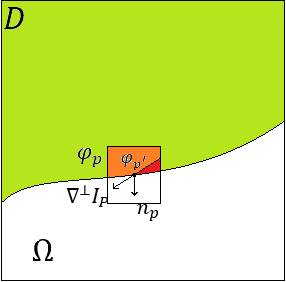
\includegraphics[scale=1]{rysunki/4_fig3}
	\caption{Oznaczenie wektorów wykorzystywanych do liczenia wartości $D(x)$.}
	\label{4_fig3} 
\end{figure}
Zgodnie z \autoref{4_fig3} funkcja $D_t$ w sposób liczbowy określa z jaką siłą izolinia obrazu uderza granicę maski. Siła ta zależna jest od gradientu jasności obrazu ${\mathrm{\nabla }}^{\bot }u_x$ oraz od orientacji względem gradientu wektora normalnego do granicy maski. Funkcja przyjmuje największą wartość w momencie, w którym wektor normalny oraz wektor izolinii są do siebie równoległe (zgodnie z iloczynem skalarnym wektorów ${\mathrm{cos} \ 0^0\ }=1)$, a człon ${\mathrm{\nabla }}^{\bot }u_x$ ma największą wartość. W przeciwieństwie do definicji terminu $C_t$ funkcję $D_t$ można zinterpretować jako człon odpowiedzialny za przyznanie wyższego priorytetu pikselowi, stanowiącemu część struktury, która według psychologii widzenia powinna być kontynuowana w głąb odrestaurowywanego obszaru. Funkcja $D_t$ wpływa ma zmniejszenie pojawiającego się w metodzie zjawiska wprowadzania niespójności obrazu. Niech funkcja $f(p)$ w punkcie obrazu $p \in D \cup \Omega$, gdzie $C(p) > 0$ przyjmuje wartość 0, a w punktach $C(p) = 0$ wartość 1, $f : (\Omega \cup D \to {0,1}$.  Wtedy korzystając z zależności \eqref{dfdx} i \eqref{dfdy} wektor normalny do granicy maski można wyznaczyć z zależności:
\begin{align}
n_p= \left[-n_{p_x}\frac{1}{l}\ ,\ -n_{p_y} \frac{1}{l}\right] =\left[-\frac{f_{i+1,j}+f_{i-1,j}}{2h}\cdot \frac{1}{l}, -\frac{f_{i,j+1} + f_{i,j-1}}{2h} \cdot \frac{1}{l}\right]
\label{KIERUNEK}
\end{align}
\begin{align}
l= \sqrt{n^2_{p_x} + n^2_{p_y}}
\label{POMKIERUNEK}
\end{align}
Dyskretyzacja równania \eqref{DataTerm} zgodnie z \eqref{u}, \eqref{v}, \eqref{KIERUNEK} i \eqref{POMKIERUNEK} w wyniku przyjmuje postać:
\begin{align}
D(p)=\ \left|u{\cdot n}_x\frac{1}{L}-v\cdot n_y\frac{1}{L}\right|
\end{align}
Znając wartości $C_t\left(x\right)$ oraz $D_t(x)$ dla każdego piksela z granicy maski można wyznaczyć wartość priorytetów $P(x)$. Na ich podstawie wybierane jest okno $p(x)$, a następnie najlepsze odwzorowanie $q_{\hat{x}}$.
Podsumowując operację wmalowywania obrazu można przedstawić w postaci następującego algorytmu. Algorytm ten należy powtarzać aż do wypełnienia wszystkich pikseli z $\mathrm{\Omega }$:
\begin{enumerate}
\item
Na podstawie \eqref{LAPLASJAN} wyznaczyć granicę maski $\mathrm{\partial }\mathrm{\Omega }$
\item
Na podstawie \eqref{PRIORITY} wyznaczyć priorytety wszystkich pikseli z granicy maski $\mathrm{\partial }\mathrm{\Omega }$
\item
Na podstawie \eqref{FROBENIUS} wyznaczyć najlepsze dopasowanie dla okna utworzonego na podstawie punktu 2 
\item
Zgodnie z \autoref{4_fig1} przepisać wartości z okna najlepszego dopasowania w restaurowany obszar, jednocześnie aktualizując wartości $C(p)$ zgodnie z zależnością:
\begin{align}
C_t\left(p\right)=C\left(\dot{p}\right)
\end{align} 
gdzie $p \in s_x$, a $C \left(\dot{p} \right)$ to malejąca wartość w każdej kolejnej iteracji.
\end{enumerate}
\section{Pojęcie głównych struktur.}
Poprawa algorytmu przedstawiona w \cite{criminisi2004region} prowadzi do polepszenia otrzymywanych wyników, lecz nie w optymalnym stopniu. W celu dalszej minimalizacji uzyskiwanych niespójności w obrazie i optymalizacji pod kątem szybkości działania algorytmów zostały wprowadzone kolejne modyfikacje: \cite{StructurePropagationManual},  \cite{malluvalasaimplementation}, \cite{SalientStrucTexProp}. 
Jednym z istotnych ulepszeń algorytmu wmalowywania w oparciu o kopiowanie fragmentów jest wprowadzenie zależności kolejności ich wstawiania w oparciu o główne struktury w obrazie.
\textbf{W niniejszej pracy zaimplementowano i sprawdzono odrestaurowywanie obrazu na podstawie zadawanych ręcznie przez użytkownika głównych linii zgodnie z \cite{StructurePropagationManual}.}
Różnica pomiędzy zwykłym algorytmem przedstawionym w \cite{criminisi2004region}, a nowym rozwiązaniem polega na wstępnej definicji przez użytkownika grupy punktów znajdujących się w masce. Najczęściej są to krzywe, które zgodnie z psychologią widzenia powinny być kontynuowane w głąb maski tworząc odpowiednie połączenia między sobą. Krzywe charakteryzują się ograniczoną grupą pikseli mogących stanowić źródło uzupełniania maski. Ograniczając pole $D^c$ dla każdej kontynuowanej krzywej (a najczęściej pary łączonych krzywych) znacznie przyspiesza się krok iteracji związany z odnalezieniem najlepszego dopasowania $p_x$ oraz $q_{\hat{x}}$. Schemat wmalowywania w oparciu o powyższy algorytm przedstawia \autoref{4_fig4}.
\begin{figure}[!h]
	\centering
	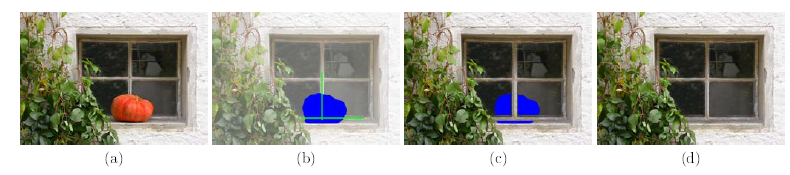
\includegraphics[scale=0.9]{rysunki/4_fig4}
	\caption{Koncepcja wmalowywania w oparciu o główne struktury obrazu. Źródło \cite{StructurePropagationManual}}
	\label{4_fig4} 
\end{figure}
\section{Automatyczne wykrywanie struktur.}
W celu zaprojektowania w pełni automatycznego programu do procesu wmalowywania opierającego się na algorytmie wprowadzonym przez Criminisi zaproponowano dodatkową analizę obrazu ograniczającą interakcję użytkownika wyłącznie do wprowadzenia maski. Autorzy w \cite{SalientStrucTexProp} proponują wykonać 2 dodatkowe kroki:
\begin{enumerate}
\item
Wyznaczenie głównych struktur obrazu.
\item
Rozwiązanie poniższych zależności:
\begin{align}
D(i,j)\triangleq IP\cdot \left[\alpha \cdot D_1\left(f^i_C,f^j_C\right)\ +\ \beta {\cdot D}_2\left(f^i_T,f^j_T\right)+\gamma {\cdot D}_3\left(f^i_{Cur},f^j_{Cur}\right)\right]
\label{SalientDistance}
\end{align}
\begin{align}
Paired\left(i,j\right)={\mathrm{arg}\ \mathop{\mathrm{min}}_{i,j\ \epsilon \mathrm{\ }\{1,..,N\}} D(i,j)\ }
\label{SalientPair}
\end{align}
\end{enumerate}
Analiza powyższych równań wykonana zostanie w sposób szczegółowy dla każdego z członów $\alpha \cdot D_1\left(f^i_C,f^j_C\right)\ $,$\ \beta {\cdot D}_2\left(f^i_T,f^j_T\right)$, oraz $\gamma {\cdot D}_3\left(f^i_{Cur},f^j_{Cur}\right)$. Uprzednim krokiem do powyższych równań według \cite{SalientStrucTexProp} jest wyznaczenie głównych struktur na podstawie obrazu wejściowego poddanego wstępnemu rozmyciu funkcją Gaussa:
\begin{align}
G\left(i,j\right)=\frac{1}{\sqrt{2\pi }\sigma }e^{\frac{i^2+j^2}{2{\sigma }^2}}
\label{rozmycieGaussa}
\end{align}
Operacji rozmycia dokonuje się poprzez operację splotu obrazu z odpowiednio wygenerowaną macierzą wyznaczoną na podstawie powyższego równania. Operacja rozmycia pozwala pozbyć się mniej znaczących krawędzi z obrazu zostawiając tylko najistotniejsze cechy, które powinny być kontynuowane w niewyznaczonym obszarze. Po operacji rozmycia autorzy w \cite{SalientStrucTexProp} proponują wykrycie głównych struktur na podstawie transformacji falkowej oraz odpowiednio wyznaczonych lokalnych maksimów dla funkcji powstałych na podstawie wspomnianej transformacji. Na podstawie przeprowadzonej operacji uzyskuje się wszystkie główne struktury obrazu. Zbiorem krawędzi poddanych analizie są ostatecznie struktury, dla których dochodzi do przecięcia ze zdefiniowaną maską $\mathrm{\Omega }$ zgodnie z \autoref{4_fig5} (jako maska traktowany jest samochód).
\begin{figure}[!h]
	\centering
	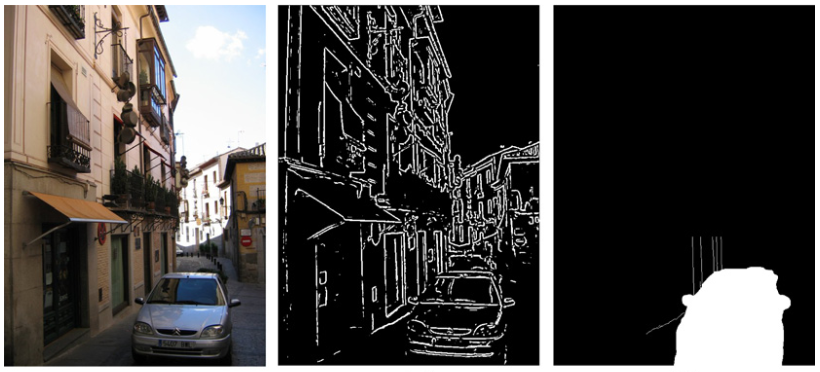
\includegraphics[scale=0.8]{rysunki/4_fig5}
	\caption{Koncepcja wmalowywania w oparciu o główne struktury obrazu. źródło \cite{StructurePropagationManual}.}
	\label{4_fig5} 
\end{figure}
Dla każdej linii stykającej się z obszarem $\mathrm{\Omega }$ wyznaczony zostaje punkt środkowy. Względem środka tego punktu tworzone jest okno  $f^i$ o wcześniej zdefiniowanym obszarze. Pierwszym członem w równaniu \eqref{SalientDistance} wyznaczonym na podstawie utworzonego okna $f^i$ jest $D_1\left(f^i_C,f^j_C\right)$. Symbole $f^i_C$ oraz $f^j_C$ stanowią posegmentowane fragmenty obrazu względem wcześniej zdefiniowanej liczby głównych, dominujących kolorów w obrazie. Dla każdego wycinka $f^i_C$ można zdefiniować zbiór punktów $(c_k,p_k)$, gdzie $c_k$ odpowiada danemu kolorowi, natomiast $p_k$ jego procentowemu udziałowi we fragmencie $f^i$, przy $k=1,\dots ,M$. Dysponując zbiorami punktów dla okien $f^i_C$,$\ f^j_C$ można liczbowo przedstawić ich poziom podobieństwa obliczając: 
\begin{align}
D_1\left(f^i_C,f^j_C\right)=IOCCD({\left(c_k,p_k\right)}_i,{\left(c_k,p_k\right)}_j
\label{colDistance}
\end{align}
Dokładna analiza oraz sposób wyznaczania podobieństwa okien $f^i$ przedstawiony jest w\cite{chen2005adaptive}.
Drugim członem w równaniu \eqref{SalientDistance} jest $D_2\left(f^i_T,f^j_T\right)$ określający stopień podobieństwa tekstur znajdujących się w utworzonych oknach $f$. Dla każdego obszaru $f^i$ wyznaczana jest macierz $MR8(f^i)$. Macierz uzyskiwana jest na podstawie odpowiedzi wybranego fragmentu obrazu na grupę 38 filtrów przedstawionych na \autoref{4_fig6}.
\begin{figure}[!h]
	\centering
	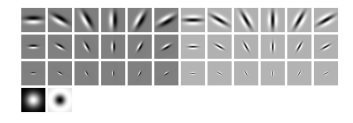
\includegraphics[scale=1]{rysunki/4_fig6}
	\caption{Bank 38 filtrów grupy MR8. źródło \cite{varma2009statistical}.}
\label{4_fig6}
\end{figure}
Przez odpowiedź obrazu na filtr należy rozumieć operację splotu z macierzą odpowiadającą definicji konkretnego filtru. W grupie filtrów $MR8$ branych pod uwagę znajduje się filtr Gaussowski, oraz filtr $LOG$ będący laplasjanem funkcji gaussowskiej. Na pozostałe 36 filtrów składają się dwie grupy filtrów utworzonych na podstawie filtru krawędziowego oraz filtru (w języku angielskim) "bar filter". Każdy z nich przedstawiony jest w sześciu orientacjach oraz trzech skalach zgodnie z rysunkiem \autoref{4_fig6}. Maksymalna odpowiedź na bazę trzydziestu ośmiu filtrów definiowana jest następująco:
\begin{align}
I_{fmax}(p)=\mathrm{max}\mathrm{}(I_{f1}(p),I_{f2}(p),\dots ,I_{f38}(p))
\end{align}
gdzie $p$ - piksel obrazu poddanego filtracji, $p\in I$, $I_{fi}$ - odpowiedź obrazu $I$ na $i$-ty filtr z bazy filtrów. Wzajemne podobieństwo wyznaczonych okien odpowiadających głównym strukturom w obrazie można wyrazić zależnością:
\begin{align}
D_2{\left(f^i_T,f^j_T\right)}_i=\frac{{\left|MR8\left(f^i\right)-MR8\left(f^j\right)\right|}_F}{250}=\frac{{\left|f^i_T-f^j_T\right|}_F}{250}
\end{align}
W powyższej zależności norma oznaczona literą $F$ oznacza normę Frobenius'a liczoną zgodnie z \eqref{FROBENIUS}.
Dokładny algorytm klasyfikacji tekstur przedstawiony został przez Manika Varma'e i Adrew Zisserman'a w \cite{varma2009statistical}. Ostatnim członem w równaniu \eqref{SalientDistance} jest człon $D_3\left(f^i_{cur},f^j_{cur}\right)$ odpowiadający liczbowej reprezentacji podobieństwa krzywizn ze zbioru głównych struktur. Autorzy w \cite{SalientStrucTexProp} nie podają sposobu wyznaczenia normy:
\begin{align}
D_3\left(f^i_{cur},f^j_{cur}\right)=\ \left|curvature_i-curvature_j\right|
\end{align}
Proponują natomiast aby każdą z wyznaczonych głównych struktur przedstawić w postaci równania wielomianu drugiego stopnia. Aproksymacji współczynników wielomianu można dokonać na podstawie rozwiązania poniższego równania macierzowego:
\begin{align}
\left[ \begin{array}{ccc}
n & \sum{x_i} & \sum{x^2_i} \\ 
\sum{x_i} & \sum{x^2_i} & \sum{x^3_i} \\ 
\sum{x^2_i} & \sum{x^3_i} & \sum{x^4_i} \end{array}
\right]\cdot \left[ \begin{array}{c}
a_0 \\ 
a_1 \\ 
a_2 \end{array}
\right]=\left[ \begin{array}{c}
\sum{y_i} \\ 
\sum{x_iy_i} \\ 
\sum{{x^2_iy}_i} \end{array}
\right]
\end{align}
gdzie $n$ określa liczbę zastosowanych par $(x_i,y_i)$, a wielomian przedstawia się w postaci:
\begin{align}
curvature_i={f_i\left(x\right)=a}_{0_i}+a_{1_i}x+a_{2_i}x^2
\end{align}
Według wyznaczonych równań, pary głównych struktur uzyskane w dalszych krokach algorytmu, propagowane są w głąb obszaru $\mathrm{\Omega }$, aż do momentu ich przecięcia. Ostatnią ważną zmienną w równaniu \eqref{SalientDistance} jest $IP$. Jest to zmienna, która przyjmuje wartość zerową, gdy badana para głównych struktur nie jest ze sobą równoległa, bądź jeden w przeciwnym wypadku. Aby uzyskać równania prostych opisujące wyznaczone krzywe można dokonać aproksymacji na podstawie transformacji Hough'a. Transformacja bazuje na wygodnej postaci równania prostej:
\begin{align}
y=\ -\frac{{\mathrm{cos} \theta \ }}{{\mathrm{sin} \theta \ }}x+\frac{r}{{\mathrm{sin} \theta \ }}
\label{HOUGHTRANSFORM}
\end{align}
Posługiwanie się parametrami $\theta $ oraz $r$ pozwala uniknąć niejednoznaczności, w przypadku opisu pionowych linii oraz umożliwia przedstawienie prostej w postaci jednego punktu w przestrzeni Hough'a. Przekształcenie z przestrzeni $D^c$ można przedstawić następująco:
\begin{figure}[!h]
	\centering
	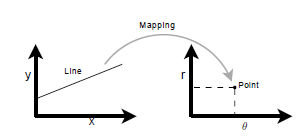
\includegraphics[scale=1]{rysunki/4_fig7}
	\caption{Odwzorowanie prostej w przestrzeni Hough’a}
\label{4_fig7}
\end{figure}
Posługując się parametrem $\theta$ określającym kąt pomiędzy wyznaczoną prostą a osią $x$ łatwo określić czy badane proste są do siebie równoległe. Aby wyznaczyć parametry prostej z równania \eqref{HOUGHTRANSFORM} zgodnie z \cite{houghTransform} należy każdemu punktowi tworzącemu prostą przypisać grupę punktów z przestrzeni Hough'a dla których wszystkie możliwe proste utworzone na ich podstawie zawierałyby badany punkt. Ostatecznie parametry prostej pochodzą z punktu, dla którego w przestrzeni Hough'a występuje największa gęstość powtarzających się punktów. Transformację przedstawia poniższy rysunek:
\begin{figure}[!h]
	\centering
	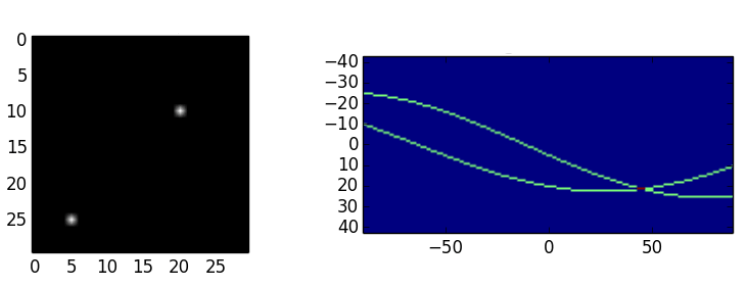
\includegraphics[scale=0.65]{rysunki/4_fig8}
	\caption{Transformacja dwóch punktów do dwóch krzywych w przestrzeni Hough'a. Punkt przecięcia definiuje prostą zawierającą dwa punkty.}
\label{4_fig8}
\end{figure}
Dokładną analizę transformacji można znaleźć w \cite{houghTransform}.
Pojawiające się współczynniki $\alpha ,\beta ,\gamma $ w równaniu \eqref{SalientDistance} stanowią wcześniej zdefiniowane wartości przypisujące procentowy wpływ poszczególnych członów na ostateczną wartość dopasowania $D(i,j)$. Według \cite{SalientStrucTexProp} najważniejszym dopasowaniem jest dopasowanie kolorów, następnie tekstur i krzywizn. Stąd należy przyjmować $\alpha >\beta >\gamma $ gdzie suma współczynników wynosi 1. W pracy zbadano powyższe rozwiązanie w ograniczeniu do wykorzystania członów $D_1\left(f^i_C,f^j_C\right)$ oraz $IP$. Człon $D_2\left(f^i_T,f^j_T\right)$ jest istotny w przypadku obrazów monochromatycznych o różnej teksturze. W przypadku obrazów kolorowych w większości przypadków linie granicy głównych struktur tworzone są poprzez gradienty kolorów. Zaletą metody jest stosowanie podzbiorów stanowiących źródło kopiowanych fragmentów w nieznane części obrazu. W uproszczeniu można to przedstawić zgodnie z rysunkiem \autoref{4_fig9}
\begin{figure}[!h]
	\centering
	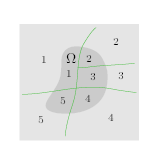
\includegraphics[scale=0.4]{rysunki/4_fig9}
	\caption{Grupowanie podzbiorów stanowiących źródło fragmentów wykorzystywanych do syntezy podzbiorów nieznanego obszaru $\boldsymbol{\mathrm{\Omega }}$. źródło \cite{StructurePropagationManual}.}
\label{4_fig9}
\end{figure}
Pomimo automatycznej metody wykrywania i kontunuowania głównych struktur algorytm wymaga wielu operacji wykonywanych zdalnie przez użytkownika, takich jak stopień rozmycia wymagany do wprowadzenia w obrazie, wielkość kopiowanych fragmentów $\psi $, czy też okien stanowiących podstawę do dobierania w pary danych struktur $f$. W przeciwieństwie do metod bazujących na rozwiązywaniu równań różniczkowych oraz metod bazujących na procesie dyfuzji proces wmalowywania opisany w aktualnym rozdziale pozbawiony jest wady w postaci rozmycia w odrestaurowanym obszarze. Jednym z problemów metody jest konieczność stosowania metody korekcji fotometrycznej zgodnie z \cite{StructurePropagationManual}, wygładzającej lokalne granice obrazu powstałe w wyniku syntezy fragmentów obrazu $q_{\hat{x}}$ w wyznaczanym obszarze $\mathrm{\Omega }$.
\chapter{Modyfikacje algorytmów}
\section{Modyfikacja algorytmu Criminisi.}
\label{ssec:crimMod}
Algorytm wypełniania fragmentami obrazu zbadano pod kątem ograniczenia źródła czerpania najlepszego dopasowania $q_{\hat{x}}$ do okna będącego otoczeniem o promieniu $s_r$ rozważanego piksela $p$. Wtedy dla $q$ zachodzi zależność $q \in \mathcal{Z}$, $\mathcal{Z} = (p + \cdot(r))$, gdzie $\cdot(s_r))$ oznacza rozmiar otaczającego okna. Zmiana odnosi się do uprzedniej definicji \eqref{qSource}.
\subsection{Modyfikacja funkcji $C_t$ }
TODO \\
Połączenie to co w VF z Crim. Zmienną $C_t$ można opisać wykorzystując przytoczoną już zależność \eqref{pewnoscVFI}.
\subsection{Modyfikacja norm.}
TODO \\
Można się również posłużyć\eqref{NLWEIGHT}, \eqref{normNNF}, \eqref{nonLocalMeans}, \eqref{nonLocalMedians} czy \eqref{nonLocalpoisson}
TODO \\
Ze względu na nieregularny kształt większości masek wyznaczenie jej granicy $\partial \mathrm{\Omega }$ można wykonać poprzez operację erozji i dylacji na funkcji $f$. Innym sposobem może być zastosowanie dyskretnego splotu funkcji $f$ z macierzą $mL$ reprezentującą Laplasjan dla siatki 8-spójnej: 
\begin{equation}
mL=\left| \begin{array}{ccc}
1 & 1 & 1 \\ 
1 & -8 & 1 \\ 
1 & 1 & 1 \end{array}
\right|
\label{LAPLASJAN}
\end{equation}
\section{Modyfikacja funkcji wagi.}
Podczas testowania algorytmu $NLCTV$ jedną z wad okazała się zbyt lokalna analiza obrazu, powodująca brak odpowiedniej kontynuacji struktury. Zwiększając parametry w postaci rozmiaru fragmentu obrazu i rozmiaru okna algorytm wprowadza zbytnie uśrednienie nie pozwalające odpowiednio kontynuować tekstury obrazu przy zniekształceniu struktury. W celu uniknięcia zjawiska rozmycia tekstur, przy jednoczesnej poprawie zdolności algorytmu do kontynuacji większych struktur zaproponowano modyfikację funkcji wagi \eqref{NLWEIGHT} do następującej postaci:
\begin{align}
\begin{aligned}
w\left(x,y\right) &= {\mathrm{exp} \left\{-\frac{G_{\sigma }*{\left|I\left(x+\ \cdot \right)-I\left(y+\ \cdot \right)\right|}^2}{r^2}\right\} }\\
&\cdot {\mathrm{exp} \left\{-\frac{G_{\sigma }*{\left|I\left(x+\ s(\cdot) \right)-I\left(y+\ s(\cdot) \right)\right|}^2}{r^2}\right\} }
\label{NLWEIGHTMODIFIED}
\end{aligned}
\end{align}
W powyższej zależności człon $s(\cdot)$ oznacza przeskalowanie  domyślnej wartości przyjętego rozmiaru fragmentu obrazu do rozmiaru $s$-krotnie większego. Edycja nie dotyczy pozostałej części  algorytmu i wpływa jedynie na wartość wagi.
\section{Modyfikacja wyznaczania wartości piksela w obrazie $u$.}
Złożoność obliczeniowa algorytmu $NLCTV$ skutkuje stosunkowo długim czasem wypełniania obrazu. W celu skrócenia czasu wyznaczania obrazu wynikowego zastosowano następującą aproksymację równania  \eqref{uNLCTV} pozwalającą uzyskać wyniki przybliżone do wyników oryginalnego algorytmu:
\begin{align}
\begin{aligned}
{{\left(u_i\right)}_l}^{k+1} &= \frac{1}{{\left({\lambda }_D\right)}_l+2\mathrm{\Theta} \sum\limits_{j\in N_i} {\left(w_i\right)}_{l,j}\ } \Biggl[2\mathrm{\Theta }\sum_{j\in N_i} {{{\left(u^k_i\right)}_j\left(w_i\right)}_{l,j}\ }\\
&+ {\left({\lambda }_D\right)}_l{\left(f_i\right)}_l\Biggr]
\end{aligned}
\label{NLH1}
\end{align}
W powyższym równaniu eliminacja zmiennych $v$ oraz $b$ pozwala znacznie ograniczyć wykorzystywaną pamięć przez programu oraz przyspieszyć działanie dzięki pominięciu obliczeń, wyrugowanych zmiennych.
\section{Połączenie metody Criminisi z funkcją wagi.}
Kolejną z pozytywnych prób modyfikacji algorytmu $NLCTV$ w pracy okazała się próba zastąpienia problemu minimalizacji energii \eqref{ENLCTV} opartej na funkcji wagi, metodą syntezy obrazu (bazującej na metodzie syntezy tekstury opisanej w \autoref{chap:StructureTextureNavierStokes}). Kroki nowego algorytmu można przedstawić w następującym schemacie:
\begin{enumerate}
\item
Ustawienie argumentów algorytmu: obraz $u$, maska obrazu $\chi$, wielkość okna $SW$, wielkość fragmentu obrazu obrazu $PS$ 
\item
Wyznaczenie funkcji wagi $w$ zgodnie z \eqref{DNLWEIGHT} dla parametrów $SW$ i $PS$ i $\chi$
\item
Powtarzanie aż do uzyskania zbioru $\Omega = \emptyset$
\begin{enumerate}[a)]
\item
Znalezienie dla każdego piksela $p \in \partial\Omega$ najlepszego dopasowania $d \in D \cap N_p$, gdzie $N_p$ zbiór pikseli z okna utworzonego dla piksela $p$, dla którego zachodzi:
\begin{large}
\begin{align}
d = \mathop{\mathrm{arg \ max}}_{t \in D \cap N_p} w(p,t)
\end{align}
\end{large}
a następnie przepisanie:
\begin{align}
u(p) = u(d)
\end{align}
\item
Pomniejszenie maski $\Omega$ o granicę $\partial\Omega$
\end{enumerate}
\end{enumerate}
Zastosowana modyfikacja pozwala na szybkie wyznaczenie wartości obrazu w szukanym obszarze $\Omega$. Przedstawiony sposób  pozwala uniknąć sytuacji, w której tworzony jest obcy kolor będący z poza gamy dostępnych kolorów w obrazie. Taki sposób wyznaczania wpływa na wartość wag obliczanych w kolejnych iteracjach i niweluje błąd wyznaczania wartości koloru z poza dostępnej gamy w kolejnych iteracjach dla $\partial \Omega$. Podobnie jak dla modelu $NLCTV$ można tutaj  zastosować modyfikację funkcji wagi $w$ zgodnie z \eqref{NLWEIGHTMODIFIED}, w celu uzyskania podobnego efektu.
\chapter{Testy algorytmów}
\section{Analizowane obrazy.}
W niniejszej pracy testom poddano następującą grupę obrazów:
\begin{longtable}[h!]{|c|c|}
    \hline
    Obraz & Dane \\ \hline

    \begin{minipage}{.65\textwidth}
    \vspace{0.5cm}
    \centering
    \includegraphics[height=5.8cm]{imgmask/kotmyszm}
    \vspace{0.5cm}
    \end{minipage}
    &
    \begin{minipage}{.35\textwidth}
	Wymiar: 500 x 375 \\
	Rozmiar maski: 28\% \\
	Nazwa: \kotmyszm
    \end{minipage} \\ \hline
    
    \begin{minipage}{.65\textwidth}
    \vspace{0.5cm}
    \centering
    \includegraphics[height=5.8cm]{imgmask/maciek1m}
    \vspace{0.5cm}
    \end{minipage}
    &
    \begin{minipage}{.35\textwidth}
	Wymiar: 410 x 308 \\
	Rozmiar maski: 28\% \\
	Nazwa: \maciekIm
    \end{minipage} \\ \hline
    
    \begin{minipage}{.65\textwidth}
    \vspace{0.5cm}
    \centering
    \includegraphics[height=5.8cm]{imgmask/Obr1m}
    \vspace{0.5cm}
    \end{minipage}
    &
    \begin{minipage}{.35\textwidth}
	Wymiar: 614 x 461 \\
	Rozmiar maski: 9\% \\
	Nazwa: \ObrIm
    \end{minipage} \\ \hline
    
    \begin{minipage}{.65\textwidth}
    \vspace{0.5cm}
    \centering
    \includegraphics[height=5.8cm]{imgmask/Obr4m}
    \vspace{0.5cm}
    \end{minipage}
    &
    \begin{minipage}{.35\textwidth}
	Wymiar: 576 x 360 \\
	Rozmiar maski: 7\% \\
	Nazwa: \ObrIVm
    \end{minipage} \\ \hline

    \begin{minipage}{.65\textwidth}
    \vspace{0.5cm}
    \centering
    \includegraphics[height=5.8cm]{imgmask/Obr5m}
    \vspace{0.5cm}
    \end{minipage}
    &
    \begin{minipage}{.35\textwidth}
	Wymiar: 650 x 570 \\
	Rozmiar maski: 28\% \\
	Nazwa: \ObrVm
    \end{minipage} \\ \hline

    \begin{minipage}{.65\textwidth}
    \vspace{0.5cm}
    \centering
    \includegraphics[height=5.8cm]{imgmask/Obr6m}
    \vspace{0.5cm}
    \end{minipage}
    &
    \begin{minipage}{.35\textwidth}
	Wymiar: 655 x 491 \\
	Rozmiar maski: 9\% \\
	Nazwa: \ObrVIm
    \end{minipage} \\ \hline
    
    \begin{minipage}{.65\textwidth}
    \vspace{0.5cm}
    \centering
    \includegraphics[height=5.8cm]{imgmask/Obr15m}
    \vspace{0.5cm}
    \end{minipage}
    &
    \begin{minipage}{.35\textwidth}
	Wymiar: 1772 x 1181 \\
	Rozmiar maski: 4.5\% \\
	Nazwa: \ObrXVm
    \end{minipage} \\ \hline

    \begin{minipage}{.65\textwidth}
    \vspace{0.5cm}
    \centering
    \includegraphics[height=5.8cm]{imgmask/Obr17m}
    \vspace{0.5cm}
    \end{minipage}
    &
    \begin{minipage}{.35\textwidth}
	Wymiar: 206 x 308 \\
	Rozmiar maski: 14\% \\
	Nazwa: \ObrXVIIm
    \end{minipage} \\ \hline

    \begin{minipage}{.65\textwidth}
    \vspace{0.5cm}
    \centering
    \includegraphics[height=5.8cm]{imgmask/Obr19m}
    \vspace{0.5cm}
    \end{minipage}
    &
    \begin{minipage}{.35\textwidth}
	Wymiar: 461 x 615 \\
	Rozmiar maski: 7\% \\
	Nazwa: \ObrXIXm
    \end{minipage} \\ \hline

    \begin{minipage}{.65\textwidth}
    \vspace{0.5cm}
    \centering
    \includegraphics[height=5.8cm]{imgmask/Obr28km}
    \vspace{0.5cm}
    \end{minipage}
    &
    \begin{minipage}{.35\textwidth}
	Wymiar: 820 x 615 \\
	Rozmiar maski: 28\% \\
	Nazwa: \ObrXXVIIIkm
    \end{minipage} \\ \hline

    \begin{minipage}{.65\textwidth}
    \vspace{0.5cm}
    \centering
    \includegraphics[height=5.8cm]{imgmask/Osoba_drugam}
    \vspace{0.5cm}
    \end{minipage}
    &
    \begin{minipage}{.35\textwidth}
	Wymiar: 2592 x 1944 \\
	Rozmiar maski: 28\% \\
	Nazwa: \OsobaDrugam
    \end{minipage} \\ \hline
    
    \begin{minipage}{.65\textwidth}
    \vspace{0.5cm}
    \centering
    \includegraphics[height=5.8cm]{imgmask/Obr13m}
    \vspace{0.5cm}
    \end{minipage}
    &
    \begin{minipage}{.35\textwidth}
	Wymiar: 1181 x 1772 \\
	Rozmiar maski: 4\% \\
	Nazwa: \ObrXIIIm
    \end{minipage} \\ \hline
    \caption{Obrazy poddane analizie.}
  \label{imgmasks}
\end{longtable}
\section{Równania mechaniki płynu.}
Wszystkie z przeprowadzonych testów wykonano w przestrzeni $CIELab$. Przykładowe wyniki  przedstawia \autoref{TabNavierStokes}. Wynikowe obrazy uzyskane schematem centralnym \eqref{NavierDiffAdvCen} w porównaniu ze schematem "do przodu" \eqref{NavierDiffAdvFor} nie wykazują znaczących różnic. W przypadku dyfuzji anizotropowej \eqref{NavierAdv}  badane w pracy  schematy dyskretyzacji pozostawiają wyniki ze zjawiskiem rozmycia w odrestaurowywanej masce i mają znikomy wpływ na dokładność wyznaczonego obrazu. Na rozmycie obrazu ma również wpływ dokładność rozwiązania równania \eqref{Poisson}. Przykładowe wyniki w zależności od parametru $h$  przedstawia \autoref{SORMethod}. Stabilność algorytmu jest zachowana przy wartości $h~1$, $h \geq1$ w przypadku wartości $dt <0.1$. W celu uzyskania dokładniejszej kontynuacji struktury należy rozważyć bardziej zaawansowane algorytmy dyskretyzacji równania mechaniki płynów, dla przykładu \cite{tschumperle2006fast}. Kontynuacja obrazu na podstawie równania mechaniki płynów nie dostarcza nielokalnego charakteru uzupełniania braków w obrazie co ogranicza kontynuację tekstury i nie pozwala odtworzyć powtarzających się szablonów.
\begin{longtable}[h!]{|c|c|}
	\hline
    \begin{minipage}{.65\textwidth}
    \vspace{0.5cm}
    \centering
    \includegraphics[height=5.8cm]{TESTY/NavierStokes/{Obr4m.pngITER_10000dt_0.015h_3pr_2tns_2021.6256}.png}
    \vspace{0.5cm}
    \end{minipage}
    &
    \begin{minipage}{.3\textwidth}
	Parametry:		
		\begin{enumerate}
			\item $dt = 0.01$
			\item $h = 3$
			\item $t = 2021.63s$
		\end{enumerate}	
    \end{minipage}  \\ \hline

    \begin{minipage}{.65\textwidth}
    \vspace{0.5cm}
    \centering
    \includegraphics[height=5.8cm]{TESTY/NavierStokes/{Obr17m.pngITER_10000dt_0.015h_3pr_2tns_3225.3982}.png}
    \vspace{0.5cm}
    \end{minipage}
    &
    \begin{minipage}{.3\textwidth}
	Parametry:		
		\begin{enumerate}
			\item $dt = 0.01$
			\item $h = 3$
			\item $t = 3225.40s$
		\end{enumerate}	
    \end{minipage}  \\ \hline

    \begin{minipage}{.65\textwidth}
    \vspace{0.5cm}
    \centering
    \includegraphics[height=5.8cm]{TESTY/NavierStokes/{maciek1m.pngITER_10000dt_0.015h_3pr_2tns_1736.7717}.png}
    \vspace{0.5cm}
    \end{minipage}
    &
    \begin{minipage}{.3\textwidth}
	Parametry:		
		\begin{enumerate}
			\item $dt = 0.01$
			\item $h = 3$
			\item $t = 1736.77s$
		\end{enumerate}	
    \end{minipage}  \\ \hline
	\caption{Wmalowywanie obrazów bazujące na metodzie zaczerpniętej z równań występujących w mechanice płynów.}
	\label{TabNavierStokes}
\end{longtable}


\begin{longtable}[h!]{|c|}
    \hline
    \begin{minipage}{.65\textwidth}
		Obraz oryginalny
    \end{minipage}  \\ \hline

    \begin{minipage}{.65\textwidth}
    \vspace{0.5cm}
    \centering
    \includegraphics[height=5.8cm]{TESTY/SOR/{SOR}.png}
    \vspace{0.5cm}
    \end{minipage} \\ \hline
    
    \begin{minipage}{.65\textwidth}
		Rozwiązanie \eqref{Poisson} metodą SOR. Parametr: $h=1$
    \end{minipage} \\ \hline

    \begin{minipage}{.65\textwidth}
    \vspace{0.5cm}
    \centering
    \includegraphics[height=5.8cm]{TESTY/SOR/{SORITER_1h_1}.png}
    \vspace{0.5cm}
    \end{minipage} \\ \hline

    \begin{minipage}{.65\textwidth}
		Rozwiązanie \eqref{Poisson} metodą SOR. Parametr: $h=10$
    \end{minipage} \\ \hline

    \begin{minipage}{.65\textwidth}
    \vspace{0.5cm}
    \centering
    \includegraphics[height=5.8cm]{TESTY/SOR/{SORITER_1h_10}.png}
    \vspace{0.5cm}
    \end{minipage} \\ \hline
    
	\caption{Wyniki obrazów uzyskane metodą $SOR$.}
	\label{SORMethod}
\end{longtable}
Dla większej wartości parametru $h$ uzyskuje się większą dokładność wyznaczonego obrazu. Niezależnie od dobrania parametru wynik generuje zjawisko rozmycia ostrych krawędzi obrazu.
\section{Segmentacja obrazu na strukturę i teksturę.}
Przykłady obrazów poddanych segmentacji przedstawia \autoref{TabSegmentation}.
\begin{longtable}[h!]{|c|c|}
    \hline
    \multicolumn{2}{|c|}{
    	Segmentacja obrazu
    } \\ \hline
    \begin{minipage}{0.5\textwidth}
    \centering
	Obraz oryginalny
    \end{minipage}
	&
    \begin{minipage}{0.5\textwidth}
    \centering
	Struktura obrazu
    \end{minipage}\\ \hline
    \multicolumn{2}{|c|}{
    \centering
    	$\lambda = 0.005$, $t=2.67s$
    } \\ \hline
    \begin{minipage}{0.5\textwidth}
    \vspace{0.5cm}
    \centering
    \includegraphics[height=3.8cm]{{imgmask/kotmyszm}.png}
    \vspace{0.5cm}
    \end{minipage}
	&
    \begin{minipage}{0.5\textwidth}
    \vspace{0.5cm}
    \centering
    \includegraphics[height=3.8cm]{{TESTY/SEGMENTACJA/kotmyszm.bmpUlambda_0.005ts_2.6707}.png}
    \vspace{0.5cm}
    \end{minipage}\\ \hline
    
    \multicolumn{2}{|c|}{
    \centering
    	$\lambda = 0.03$, $t=0.52s$
    } \\ \hline
    \begin{minipage}{0.5\textwidth}
    \vspace{0.5cm}
    \centering
    \includegraphics[height=3.8cm]{{imgmask/Obr17m}.png}
    \vspace{0.5cm}
    \end{minipage}
	&
    \begin{minipage}{0.5\textwidth}
    \vspace{0.5cm}
    \centering
    \includegraphics[height=3.8cm]{{TESTY/SEGMENTACJA/Obr17m.pngUlambda_0.03ts_0.52276}.png}
    \vspace{0.5cm}
    \end{minipage}\\ \hline
    
    \multicolumn{2}{|c|}{
    \centering
    	$\lambda = 0.03$, $t=2.99s$
    } \\ \hline
    \begin{minipage}{0.5\textwidth}
    \vspace{0.5cm}
    \centering
    \includegraphics[height=3.8cm]{{imgmask/Obr4m}.png}
    \vspace{0.5cm}
    \end{minipage}
	&
    \begin{minipage}{0.5\textwidth}
    \vspace{0.5cm}
    \centering
    \includegraphics[height=3.8cm]{{TESTY/SEGMENTACJA/Obr4m.pngUlambda_0.03ts_2.9892}.png}
    \vspace{0.5cm}
    \end{minipage}\\ \hline
	\caption{Segmentacja obrazu na strukturę i teksturę.}
	\label{TabSegmentation}
\end{longtable}
Czas trwania segmentacji obrazu nie przekracza kilku sekund. Zmniejszając parametr $\lambda$ otrzymujemy większą gładkość wynikowej struktury obrazu. Algorytm segmentacji obrazu wykorzystywany jest jako poprzedzający proces wmalowywania oparty na oddzielnej syntezie tekstury i struktury, przykładem są metody przedstawione w \cite{NavierStokesAndTexturePropagation}. Wyniki algorytmu wykorzystującego metodę Criminisi do wyznaczenia tekstury oraz równania Naviera-Stokesa wyznaczenia struktury przedstawia \autoref{TabNavierStokesSegm}. W tabeli dokonano porównania z algorytmem bez wcześniejszej segmentacji obrazu.
\begin{longtable}[h!]{|c|c|}
    \hline
    \begin{minipage}{0.5\textwidth}
    \centering
	Metoda bez segmentacji
    \end{minipage}
	&
    \begin{minipage}{0.5\textwidth}
    \centering
	Metoda z segmentacją
    \end{minipage}\\ \hline
    
    \begin{minipage}{0.5\textwidth}
    \vspace{0.5cm}
    \centering
    Parametry: \\
	$dt = 0.01$ \\
	$h = 3$ \\
	$t = 2021.63s$ \\
	Iteracje: 10000 \\
    \vspace{0.5cm}
    \end{minipage}
    &
    \begin{minipage}{0.5\textwidth}
    \vspace{0.5cm}
    \centering
    Parametry: \\
	$dt = 0.01$ \\
	$h = 1$ \\
	$t_{NS} = 3310.80s$ \\
	$t_{CRIM} = 58.26s$ \\
	Iteracje: 16000 \\
    \vspace{0.5cm}
    \end{minipage}\\ \hline

    \begin{minipage}{0.5\textwidth}
    \vspace{0.5cm}
    \centering
    \includegraphics[height=3.8cm]{TESTY/NavierStokes/{Obr4m.pngITER_10000dt_0.015h_3pr_2tns_2021.6256}.png}
    \vspace{0.5cm}
    \end{minipage}
	&
    \begin{minipage}{0.5\textwidth}
    \vspace{0.5cm}
    \centering
    \includegraphics[height=3.8cm]{{TESTY/NavierStokes/Obr4m.pngITER_16000dt_0.01h_1pr_2ts_0.37671tns_3310.8032tt_58.261}.png}
    \vspace{0.5cm}
    \end{minipage}\\ \hline

    \begin{minipage}{0.5\textwidth}
    \vspace{0.5cm}
    \centering
    Parametry: \\
	$dt = 0.01$ \\
	$h = 3$ \\
	$t = 3225.40s$ \\
	Iteracje: 10000 \\
    \vspace{0.5cm}
    \end{minipage}
    &
    \begin{minipage}{0.5\textwidth}
    \vspace{0.5cm}
    \centering
    Parametry: \\
	$dt = 0.01$ \\
	$h = 1$ \\
	$t_{NS} = 526.76s$ \\
	$t_{CRIM} = 26.03s$ \\
	Iteracje: 10000
    \vspace{0.5cm}
    \end{minipage}\\ \hline

    \begin{minipage}{0.5\textwidth}
    \vspace{0.5cm}
    \centering
    \includegraphics[height=3.8cm]{TESTY/NavierStokes/{Obr17m.pngITER_10000dt_0.015h_3pr_2tns_3225.3982}.png}
    \vspace{0.5cm}
    \end{minipage}
	&
    \begin{minipage}{0.5\textwidth}
    \vspace{0.5cm}
    \centering
    \includegraphics[height=3.8cm]{TESTY/NavierStokes/{Obr17m.pngdt_0.01h_1pr_3ts_0.49582tns_526.7624tt_26.033}.png}
    \vspace{0.5cm}
    \end{minipage}\\ \hline

	\caption{Porównanie wyników uzyskanych metodą rozwiązania równania Navier'a-Stokes'a do metody z algorytmem segmentacji.}
	\label{TabNavierStokesSegm}
\end{longtable}
Oddzielna synteza tekstury pozwala na jej kontynuację wgłąb maski. Efekt rozmycia głównego algorytmu odrestaurowania struktury negatywnie wpływa na jakość wynikowego obszaru. Proces dodania tekstury może prowadzić do powstania nieprawidłowych wyników w postaci nowych kolorów obrazu w przypadku wstawiania tekstur pochodzących z innych struktur danego obrazu. Wadą jest również obcy element tekstury w danej strukturze.
\section{Uzupełnianie kawałkami obrazu.}
\subsection{Metoda Criminisi.}
Wszystkie z przeprowadzonych testów wykonano w przestrzeni $RGB$. Dystans pomiędzy fragmentami wyznaczono według przytoczonej w poświęconym metodzie rozdziale normy Frobenius'a \eqref{FROBENIUS2}. Przykładowe wyniki przedstawia poniższa tabela:
\begin{longtable}[h!]{|c|c|}
    \hline
    Obraz & Dane \\ \hline

    \begin{minipage}{.65\textwidth}
    \vspace{0.5cm}
    \centering
    \includegraphics[height=5.8cm]{TESTY/CRIM2004/Obr17/{Obr17m.pngpr_3sr_8006alfa_0.2t_31.7202}.png}
    \vspace{0.5cm}
    \end{minipage}
    &
    \begin{minipage}{.35\textwidth}
    \begin{itemize}
        \item pr: 3
        \item Czas: 31.72s
    \end{itemize}
    \end{minipage} \\ \hline
    
    \begin{minipage}{.65\textwidth}
    \vspace{0.5cm}
    \centering
    \includegraphics[height=5.8cm]{TESTY/CRIM2004/Obr17/{Obr17m.pngpr_15sr_8006alfa_0.2t_22.4205}.png}
    \vspace{0.5cm}
    \end{minipage}
    &
    \begin{minipage}{.35\textwidth}
    \begin{itemize}
        \item pr: 15
        \item Czas: 22.42s
    \end{itemize}
    \end{minipage} \\ \hline  
    
    \begin{minipage}{.65\textwidth}
    \vspace{0.5cm}
    \centering
    \includegraphics[height=5.8cm]{TESTY/CRIM2004/Obr17/{Obr17m.pngpr_23sr_8006alfa_0.2t_20.7783}.png}
    \vspace{0.5cm}
    \end{minipage}
    &
    \begin{minipage}{.35\textwidth}
    \begin{itemize}
        \item pr: 23
        \item Czas: 20.77s
    \end{itemize}
    \end{minipage} \\ \hline
    
    \begin{minipage}{.65\textwidth}
    \vspace{0.5cm}
    \centering
    \includegraphics[height=5.8cm]{TESTY/CRIM2004/Obr4/{Obr4m.pngpr_3sr_8010alfa_0.2t_213.2492}.png}
    \vspace{0.5cm}
    \end{minipage}
    &
    \begin{minipage}{.35\textwidth}
    \begin{itemize}
        \item pr: 3
        \item Czas: 213.25s
    \end{itemize}
    \end{minipage} \\ \hline
    
    \begin{minipage}{.65\textwidth}
    \vspace{0.5cm}
    \centering
    \includegraphics[height=5.8cm]{TESTY/CRIM2004/Obr4/{Obr4m.pngpr_15sr_8010alfa_0.2t_113.4021}.png}
    \vspace{0.5cm}
    \end{minipage}
    &
    \begin{minipage}{.35\textwidth}
    \begin{itemize}
        \item pr: 15
        \item Czas: 113.40s
    \end{itemize}
    \end{minipage} \\ \hline  
    
    \begin{minipage}{.65\textwidth}
    \vspace{0.5cm}
    \centering
    \includegraphics[height=5.8cm]{TESTY/CRIM2004/Obr4/{Obr4m.pngpr_23sr_8010alfa_0.2t_134.3072}.png}
    \vspace{0.5cm}
    \end{minipage}
    &
    \begin{minipage}{.35\textwidth}
    \begin{itemize}
        \item pr: 23
        \item Czas: 134.31s
    \end{itemize}
    \end{minipage} \\ \hline
    
    \begin{minipage}{.65\textwidth}
    \vspace{0.5cm}
    \centering
    \includegraphics[height=5.8cm]{TESTY/CRIM2004/Obr19/{Obr19m.pngpr_3sr_8011alfa_0.2t_294.2353}.png}
    \vspace{0.5cm}
    \end{minipage}
    &
    \begin{minipage}{.35\textwidth}
    \begin{itemize}
        \item pr: 3
        \item Czas: 294.24s
    \end{itemize}
    \end{minipage} \\ \hline
    
    \begin{minipage}{.65\textwidth}
    \vspace{0.5cm}
    \centering
    \includegraphics[height=5.8cm]{TESTY/CRIM2004/Obr19/{Obr19m.pngpr_11sr_8011alfa_0.2t_181.0897}.png}
    \vspace{0.5cm}
    \end{minipage}
    &
    \begin{minipage}{.35\textwidth}
    \begin{itemize}
        \item pr: 11
        \item Czas: 181.10s
    \end{itemize}
    \end{minipage} \\ \hline  
    
    \begin{minipage}{.65\textwidth}
    \vspace{0.5cm}
    \centering
    \includegraphics[height=5.8cm]{TESTY/CRIM2004/Obr19/{Obr19m.pngpr_23sr_8011alfa_0.2t_196.3067}.png}
    \vspace{0.5cm}
    \end{minipage}
    &
    \begin{minipage}{.35\textwidth}
    \begin{itemize}
        \item pr: 23
        \item Czas: 196.31s
    \end{itemize}
    \end{minipage} \\ \hline
    
    \begin{minipage}{.65\textwidth}
    \vspace{0.5cm}
    \centering
    \includegraphics[height=5.8cm]{TESTY/CRIM2004/Obr13/{Obr13m.pngpr_3sr_8012alfa_0.2t_565.4799}.png}
    \vspace{0.5cm}
    \end{minipage}
    &
    \begin{minipage}{.35\textwidth}
    \begin{itemize}
        \item pr: 3
        \item Czas: 565.48s
    \end{itemize}
    \end{minipage} \\ \hline
    
    \begin{minipage}{.65\textwidth}
    \vspace{0.5cm}
    \centering
    \includegraphics[height=5.8cm]{TESTY/CRIM2004/Obr13/{Obr13m.pngpr_11sr_8012alfa_0.2t_294.7297}.png}
    \vspace{0.5cm}
    \end{minipage}
    &
    \begin{minipage}{.35\textwidth}
    \begin{itemize}
        \item pr: 11
        \item Czas: 294.73s
    \end{itemize}
    \end{minipage} \\ \hline  
    
    \begin{minipage}{.65\textwidth}
    \vspace{0.5cm}
    \centering
    \includegraphics[height=5.8cm]{TESTY/CRIM2004/Obr13/{Obr13m.pngpr_23sr_8012alfa_0.2t_328.5629}.png}
    \vspace{0.5cm}
    \end{minipage}
    &
    \begin{minipage}{.35\textwidth}
    \begin{itemize}
        \item pr: 23
        \item Czas: 328.56s
    \end{itemize}
    \end{minipage} \\ \hline
    
  \caption{Wyniki metody Criminisi.}
  \label{CRIMTEST}
\end{longtable}
Wyniki przedstawione w tabeli wyznaczono dla optymalnego ustawienia parametru $\alpha=0.2$. Biorąc pod uwagę charakter działania algorytmu i błędy jakie powstają przy jego zastosowaniu zmiana wspomnianego parametru w ogólnym rozważaniu nie wpływa na końcowe obrazy. W zależności od rozpatrywanego obrazu rozmiar fragmentu obrazu może wpływać na odpowiedniość syntezy struktury. W przypadku \ObrXVIIm \ mały rozmiar fragmentu obrazu skutkuje w odpowiedniej kontynuacji dachu budynku. W przypadku \ObrIVm \ średni wymiar fragmentu obrazu pozwala na odpowiednią syntezę plaży. W przypadku obrazu \ObrVIm \ największy rozmiar fragmentu obrazu zagwarantował dla obserwatora względnie najbliższe odtworzenie zawartości maski. W ogólnym rozrachunku metoda w każdym z wyników wprowadza wadę w postaci nieprawidłowego elementu w danej ze struktur obrazu. 
\subsection{Główne struktury obrazu.}
W celu zminimalizowania efektu zgodnie z \cite{StructurePropagationManual} algorytm wmalowywania przebadano pod kątem priorytetowego wypełnienia głównych struktur obrazu zgodnie z wytycznymi wprowadzonymi manualnie przez użytkownika. Punkty linii głównej struktury znajdującej się w obszarze maski stanowią miejsca, które wypełniane są priorytetowo.

\begin{longtable}[h!]{|c|c|}
    \hline
    Obraz & Dane \\ \hline

    \begin{minipage}{.65\textwidth}
    \vspace{0.5cm}
    \centering
    \includegraphics[height=5.8cm]{TESTY/SALCRIM2004/SALIENT/{5_9_Obr6m}.png}
    \vspace{0.5cm}
    \end{minipage}
    &
    \begin{minipage}{.35\textwidth}
    \begin{itemize}
        \item pr: 9
        \item Główne struktury: 5
    \end{itemize}
    \end{minipage} \\ \hline

    \begin{minipage}{.65\textwidth}
    \vspace{0.5cm}
    \centering
    \includegraphics[height=5.8cm]{TESTY/SALCRIM2004/SALIENT/{4_8_Obr13m}.png}
    \vspace{0.5cm}
    \end{minipage}
    &
    \begin{minipage}{.35\textwidth}
    \begin{itemize}
        \item pr: 8
        \item Główne struktury: 4
    \end{itemize}
    \end{minipage} \\ \hline

    \begin{minipage}{.65\textwidth}
    \vspace{0.5cm}
    \centering
    \includegraphics[height=5.8cm]{TESTY/SALCRIM2004/SALIENT/{3_4_Obr17m}.png}
    \vspace{0.5cm}
    \end{minipage}
    &
    \begin{minipage}{.35\textwidth}
    \begin{itemize}
        \item pr: 4
        \item Główne struktury: 3
    \end{itemize}
    \end{minipage} \\ \hline

    \begin{minipage}{.65\textwidth}
    \vspace{0.5cm}
    \centering
    \includegraphics[height=5.8cm]{TESTY/SALCRIM2004/SALIENT/{1_12_Obr19m}.png}
    \vspace{0.5cm}
    \end{minipage}
    &
    \begin{minipage}{.35\textwidth}
    \begin{itemize}
        \item pr: 12
        \item Główne struktury: 1
    \end{itemize}
    \end{minipage} \\ \hline
        
	\caption{Główne struktury testowanych obrazów manualnie wprowadzone przez użytkownika.}
\end{longtable}
Linie granic głównych struktur przedstawiono kolorem czerwonym. Część wspólna obrazu oryginalnego poza maską wraz z linią głównej struktury stanowią zbiór, z którego pobierane jest najlepsze dopasowanie. Wartość $p_r$ manualnie ustawiono na minimalną wartość zdolną zachować właściwości charakterystyczne dla danej granicy w pełnym zakresie linii. Pośrednie wyniki wypełniania struktur przedstawiono w tabeli:

\begin{longtable}[h!]{|c|c|}
    \hline
    Obraz & Dane \\ \hline

    \begin{minipage}{.65\textwidth}
    \vspace{0.5cm}
    \centering
    \includegraphics[height=5.8cm]{TESTY/SALCRIM2004/TESTY/Obr6/{5_9_Obr6m.pngpr_9sr_100000alfa_0.2t_0.49515}.png}
    \vspace{0.5cm}
    \end{minipage}
    &
    \begin{minipage}{.35\textwidth}
    \begin{itemize}
        \item Czas: 0.50s
        \item Procent wyznaczonej maski: 32.1 \%
    \end{itemize}
    \end{minipage} \\ \hline

    \begin{minipage}{.65\textwidth}
    \vspace{0.5cm}
    \centering
    \includegraphics[height=5.8cm]{TESTY/SALCRIM2004/TESTY/Obr13/{4_8_Obr13m.pngpr_8sr_100000alfa_0.2t_0.31031}.png}
    \vspace{0.5cm}
    \end{minipage}
    &
    \begin{minipage}{.35\textwidth}
    \begin{itemize}
        \item Czas: 0.31s
        \item Procent wyznaczonej maski: 16.27 \%
    \end{itemize}
    \end{minipage} \\ \hline

    \begin{minipage}{.65\textwidth}
    \vspace{0.5cm}
    \centering
    \includegraphics[height=5.8cm]{TESTY/SALCRIM2004/TESTY/Obr17/{3_4_Obr17m.pngpr_4sr_12alfa_0.2t_0.080489}.png}
    \vspace{0.5cm}
    \end{minipage}
    &
    \begin{minipage}{.35\textwidth}
    \begin{itemize}
        \item Czas: 0.08s
        \item Procent wyznaczonej maski: 12.24 \%
    \end{itemize}
    \end{minipage} \\ \hline

    \begin{minipage}{.65\textwidth}
    \vspace{0.5cm}
    \centering
    \includegraphics[height=5.8cm]{TESTY/SALCRIM2004/TESTY/Obr19/{1_12_Obr19m.pngpr_12sr_100000alfa_0.2t_0.36266}.png}
    \vspace{0.5cm}
    \end{minipage}
    &
    \begin{minipage}{.35\textwidth}
    \begin{itemize}
        \item Czas: 0.36s
        \item Procent wyznaczonej maski: 22.85 \%
    \end{itemize}
    \end{minipage} \\ \hline
        
	\caption{Wynik wyznaczania głównych struktur testowanych obrazów.}
\end{longtable}
Wyznaczenie głównych struktur w każdym z testowych obrazów nie wymagało czasu obliczeniowego dłuższego niż $1s$. W uproszeniu można przyjąć, że algorytm pozwala oszczędzić czas potrzebny na proces wmalowywania równy procentowi wyznaczonej maski z całkowitego czasu oryginalnej metody Criminisi. Ostatecznie przykładowe wyniki przedstawia  tabela:

\begin{longtable}[h!]{|c|c|}
    \hline
    Obraz & Dane \\ \hline

    \begin{minipage}{.65\textwidth}
    \vspace{0.5cm}
    \centering
    \includegraphics[height=5.8cm]{TESTY/SALCRIM2004/TESTY/Obr6/{5_9_Obr6m.pngpr_9sr_63alfa_0.2t_12.0559}.png}
    \vspace{0.5cm}
    \end{minipage}
    &
    \begin{minipage}{.35\textwidth}
    \begin{itemize}
    	\item pr: 9
        \item Czas: 12.05s
    \end{itemize}
    \end{minipage} \\ \hline

    \begin{minipage}{.65\textwidth}
    \vspace{0.5cm}
    \centering
    \includegraphics[height=5.8cm]{TESTY/SALCRIM2004/TESTY/Obr13/{4_8_Obr13m.pngpr_8sr_56alfa_0.2t_16.2741}.png}
    \vspace{0.5cm}
    \end{minipage}
    &
    \begin{minipage}{.35\textwidth}
    \begin{itemize}
    	\item pr: 8
        \item Czas: 16.27s
    \end{itemize}
    \end{minipage} \\ \hline

    \begin{minipage}{.65\textwidth}
    \vspace{0.5cm}
    \centering
    \includegraphics[height=5.8cm]{TESTY/SALCRIM2004/TESTY/Obr17/{3_4_Obr17m.pngpr_4sr_12alfa_0.2t_1.5704}.png}
    \vspace{0.5cm}
    \end{minipage}
    &
    \begin{minipage}{.35\textwidth}
    \begin{itemize}
    	\item pr: 4
        \item Czas: 1.57s
    \end{itemize}
    \end{minipage} \\ \hline

    \begin{minipage}{.65\textwidth}
    \vspace{0.5cm}
    \centering
    \includegraphics[height=5.8cm]{TESTY/SALCRIM2004/TESTY/Obr19/{1_12_Obr19m.pngpr_12sr_84alfa_0.2t_12.8458}.png}
    \vspace{0.5cm}
    \end{minipage}
    &
    \begin{minipage}{.35\textwidth}
    \begin{itemize}
    	\item pr: 12
        \item Czas: 12.85s
    \end{itemize}
    \end{minipage} \\ \hline
        
	\caption{Wynik wyznaczania głównych struktur testowanych obrazów.}
	\label{CrimSalStructRes}
\end{longtable}

Wszystkie przedstawione wyniki otrzymano ograniczając okno poszukiwań zgodnie z \autoref{ssec:crimMod} przyjmując jako parametr $s_r = 3 \cdot 	p_r$. W przypadku obrazów: \ObrVIm , \ObrXVIIm \ i \ObrXIXm \ wyniki w porównaniu do \autoref{CRIMTEST} posiadają lepszą syntezę głównych struktur, a ograniczenie okna poszukiwania przyspiesza o rząd wielkości czas wyznaczenia głównego obrazu. W przypadku \ObrXVm \ i \ObrXIIIm \ pomimo wstępnej syntezy głównych struktur nie udało się uniknąć błędów w postaci obcych wartości w różnych strukturach obrazu. Ograniczenie okna poszukiwania może wprowadzać dodatkowe błędy w przypadku niejednoznaczności struktur znajdujących się w pobliżu granicy maski. Rozważając prawą część maski \ObrXVIIm \ algorytm wypełniania ogranicza źródło wzorca do błędnego źródła zawierającego część pozostawionej w obrazie postaci (postać z prawej strony obrazu traktowana jest jako niejednoznaczność). Wadą algorytmu wypełniania jest konieczność dodatkowej korekcji fotometrycznej uzyskanego wyniku zgodnie z \cite{StructurePropagationManual} przedstawionym na \autoref{7_fig1}. 
\begin{figure}[!h]
	\centering
	\includegraphics[scale=0.5]{rysunki/7_fig1}
	\caption{Korekcja fotometryczna obrazu w przypadku propagacji głównych struktur obrazu. Źródło \cite{StructurePropagationManual}.}
	\label{7_fig1} 
\end{figure}
Ograniczenie błędów w postaci nieodpowiedniej syntezy struktur obrazu w badaniach korygowane jest poprzez wprowadzanie modyfikacji normy \eqref{FROBENIUS2} uwzględniającej wartości posegmentowanego obrazu, bądź dodatkowej wyznaczanej wartości $\nabla I$. Błąd w największym stopniu ograniczyć można poprzez dodatkowy wejściowy parametr algorytmu w postaci dodatkowej maski $\Omega '$ definiowanej przez użytkownika stanowiącej zbiór pikseli, które nie powinny pojawić się we wmalowywanym obszarze. Niech:
\begin{equation}
{\lambda }'\left(x\right)=\left\{ \begin{array}{c}
0\ x\ \epsilon \ \mathrm{\Omega } \\ 
1\ x\ \epsilon \ D/\mathrm{\Omega } \end{array}
\right\}
\end{equation}
Wtedy dla każdego ${\varphi }_q$ zachodzi warunek:
\begin{align}
\forall_{x \in {\varphi }_q}: {\lambda }'(x) = 1
\end{align}
\subsection{Automatyczne wykrywanie struktur.}
Autorzy w \cite{SalientStrucTexProp} nie przedstawiają dokładnego sposobu wyznaczania głównych struktur, łączenia w pary, a następnie wyznaczania równań kontynuacji w obszar maski. Algorytm opisany w pracy zależy od wielu zmiennych definiowanych przez użytkownika mających wpływ na ostateczny wynik, takich jak:
\begin{itemize}
\item parametry filtru usuwającego mniej znaczące krawędzie obrazu
\item ilość głównych kolorów na które zostanie posegmentowany obraz
\item rozmiar okna otaczający główną strukturę brany pod uwagę podczas wyznaczania podobieństwa kolorów \eqref{colDistance}
\item waga poszczególnych członów w równaniu \eqref{SalientDistance} mające wpływ na parowanie struktur
\end{itemize}
Dobór żadnego z parametrów nie jest automatyczny i zależy on rozpatrywanego obrazu. Problematyczność doboru parametrów i dokładność uzyskiwanych wyników potwierdziły konieczność znacznie głębszej analizy problemu. Dokładność wyników uzyskanych w poprzednim podrozdziale (przy manualnym oznaczaniu głównych struktur) w stosunku do wymaganego stopnia analizy skłoniły autora tej pracy magisterskiej do badań pozostałych algorytmów.
\section{Nielokalny model NLCTV.}
\subsection{Modyfikacja wyznaczania wartości piksela w obrazie $u$.}
Porównanie wyników algorytmu oryginalnego i uproszczonego przedstawia \autoref{NLCTVVSNLHI}. Podobieństwo obrazów mierzy się współczynnikiem:
\begin{align}
f = \frac{100}{256}\frac{1}{n| \Omega |} \sum^c_{k=1}{\sum^m_{i=1}{\sum^n_{j=1}{ | I_1(i,j,k)-I_2(i,j,k) |}}} %
\end{align}
gdzie $n$ oznacza liczbę warstw obrazu tworzących kolor, $m, \ n$ to rozmiary obrazu, $|\Omega|$ to pole obszaru maski. Do porównania algorytmów wykorzystano dodatkowo badaną grupę obrazów przedstawioną w \autoref{NLCTVVSNLHIIM}.

\begin{longtable}[h!]{| c | c |}
    \hline
    Obraz & Dane \\ \hline

    \begin{minipage}{.65\textwidth}
    \vspace{0.5cm}
    \centering
    \includegraphics[height=4cm]{TESTY/NLCTVNLH1/IM/bar}
    \vspace{0.5cm}
    \end{minipage}
    &
    \begin{minipage}{.35\textwidth}
	Wymiary obrazu: 81 x 81 \\
	Rozmiar maski: 10\% \\
	Nazwa: \XXVIII
    \end{minipage} \\ \hline

    \begin{minipage}{.65\textwidth}
    \vspace{0.5cm}
    \centering
    \includegraphics[height=4cm]{TESTY/NLCTVNLH1/IM/TEST}
    \vspace{0.5cm}
    \end{minipage}
    &
    \begin{minipage}{.35\textwidth}
	Wymiar: 113 x 66 \\
	Rozmiar maski: 6\% \\
	Nazwa: \TEST
    \end{minipage} \\ \hline
    
    \begin{minipage}{.65\textwidth}
    \vspace{0.5cm}
    \centering
    \includegraphics[height=4cm]{TESTY/NLCTVNLH1/IM/Wood}
    \vspace{0.5cm}
    \end{minipage}
    &
    \begin{minipage}{.35\textwidth}
	Wymiar: 134 x 81 \\
	Rozmiar maski: 11\% \\
	Nazwa: \Wood
    \end{minipage} \\ \hline
  \caption{Dodatkowa grupa obrazów testowych dla nielokalnego modelu $NLCTV$.}
  \label{NLCTVVSNLHIIM}
\end{longtable}

\begin{longtable}[h!]{|c|c|}
    \hline
    Oryginalny & Uproszczony \\ \hline
    
    \multicolumn{2}{|c|}{
    	Parametry:  $h=2$, $p_r=2$, $s_r=4$, $\lambda=0.01$, $\sigma=0.5$
    } \\

    \multicolumn{2}{|c|}{
    	Wyniki: $t_1=150.07$, $t_2=13.06$, $f=0.31$\%
    } \\ \hline
    
    \begin{minipage}{0.5\textwidth}
    \vspace{0.5cm}
    \centering
    \includegraphics[height=3.8cm]{{TESTY/NLCTVNLH1/ORIG/bh_2t_150.07}.png}
    \vspace{0.5cm}
    \end{minipage}
    &
    \begin{minipage}{0.5\textwidth}
    \vspace{0.5cm}
    \centering
    \includegraphics[height=3.8cm]{{TESTY/NLCTVNLH1/NLH1/bh_2_t_13.06}.png}
    \vspace{0.5cm}
    \end{minipage} \\ \hline
    
    \multicolumn{2}{|c|}{
    	Parametry:  $h=15$, $p_r=2$, $s_r=4$, $\lambda=0.01$, $\sigma=0.5$
    } \\

    \multicolumn{2}{|c|}{
    	Wyniki: $t_1=172.46$, $t_2=13.99$, $f=2.41$\%
    } \\ \hline

    \begin{minipage}{0.5\textwidth}
    \vspace{0.5cm}
    \centering
    \includegraphics[height=3.8cm]{{TESTY/NLCTVNLH1/ORIG/bh_15_t_172.46}.png}
    \vspace{0.5cm}
    \end{minipage}
    &
    \begin{minipage}{0.5\textwidth}
    \vspace{0.5cm}
    \centering
    \includegraphics[height=3.8cm]{{TESTY/NLCTVNLH1/NLH1/bh_15_t_13.99}.png}
    \vspace{0.5cm}
    \end{minipage} \\ \hline
    
    \multicolumn{2}{|c|}{
    	Parametry:  $h=2$, $p_r=2$, $s_r=4$, $\lambda=0.01$, $\sigma=0.5$
    } \\ 

    \multicolumn{2}{|c|}{
    	Wyniki: $t_1=219.95$ $t_2=12.96$ $f=0.8$\%
    } \\ \hline

    \begin{minipage}{0.5\textwidth}
    \vspace{0.5cm}
    \centering
    \includegraphics[height=3.8cm]{{TESTY/NLCTVNLH1/ORIG/th_2_t_219.95}.png}
    \vspace{0.5cm}
    \end{minipage}
    &
    \begin{minipage}{0.5\textwidth}
    \vspace{0.5cm}
    \centering
    \includegraphics[height=3.8cm]{{TESTY/NLCTVNLH1/NLH1/th_2t_12.96}.png}
    \vspace{0.5cm}
    \end{minipage} \\ \hline
    
    \multicolumn{2}{|c|}{
    	Parametry:  $h=15$, $p_r=2$, $s_r=4$, $\lambda=0.01$, $\sigma=0.5$
    } \\   

    \multicolumn{2}{|c|}{
    	Wyniki: $t_1=227.01$ $t_2=13.13$ $f=2.2$\%
    } \\ \hline    

    \begin{minipage}{0.5\textwidth}
    \vspace{0.5cm}
    \centering
    \includegraphics[height=3.8cm]{{TESTY/NLCTVNLH1/ORIG/th_10_t_227.01}.png}
    \vspace{0.5cm}
    \end{minipage}
    &
    \begin{minipage}{0.5\textwidth}
    \vspace{0.5cm}
    \centering
    \includegraphics[height=3.8cm]{{TESTY/NLCTVNLH1/NLH1/th_10_t_13.13}.png}
    \vspace{0.5cm}
    \end{minipage} \\ \hline

    \multicolumn{2}{|c|}{
    	Parametry:  $h=0.5$, $p_r=7$, $s_r=15$, $\lambda=0.01$, $\sigma=0.5$
    } \\  

    \multicolumn{2}{|c|}{
    	Wyniki: $t_1=3870.58$ $t_2=122.32$ $f=0.13$\%
    } \\ \hline    
    
    \begin{minipage}{0.5\textwidth}
    \vspace{0.5cm}
    \centering
    \includegraphics[scale=1]{{TESTY/NLCTVNLH1/ORIG/nlctvgs_r_15p_r7h_0.5sw_1_t_3870.584639}.png}
    \vspace{0.5cm}
    \end{minipage}
    &
    \begin{minipage}{0.5\textwidth}
    \vspace{0.5cm}
    \centering
    \includegraphics[scale=1]{{TESTY/NLCTVNLH1/NLH1/nlh1ws_r_15p_r7h_0.5sw_1_t_122.321}.png}
    \vspace{0.5cm}
    \end{minipage} \\ \hline
  
	\caption{Wynik wyznaczania głównych struktur testowanych obrazów.}
	\label{NLCTVVSNLHI}
\end{longtable}
Maksymalny procentowy błąd $f$ w przytoczonych testach nie przekracza wartości 3\% i można uznać go za pomijalny. Różnica pomiędzy obrazami rośnie wraz ze wzrostem współczynnika $h$. Wizualne dostrzeżenie różnicy w obrazach otrzymanych przez zastosowanie wspomnianych algorytmów jest niemal niemożliwe. Wszystkie z pozostałych testów wykonano dla algorytmu uproszczonego. Czasy uzyskania wyników różnią się o rząd wielkości. Uproszczony algorytm w znacznym stopniu przyspiesza algorytm wmalowywania. Przykładowe wyniki dla różnych parametrów algorytmu przedstawia tabela \autoref{NLH1Tab}.

\begin{longtable}[h!]{|c|c|}
    \hline
    \multicolumn{2}{|c|}{
    	Obrazy
    } \\ \hline 
    \multicolumn{2}{|c|}{
		Wpływ parametru $h$ na odwzorowanie tekstur i struktur
    } \\ \hline 
    \begin{minipage}{0.5\textwidth}
    \vspace{0.5cm}
    \centering
    Parametry: \\
    $s_r$: 25 \\
    $p_r$: 10 \\
    $h$: 2 \\
    Wyniki: \\ 
    Czas: 2041.85s 
    \vspace{0.5cm}
    \end{minipage}
    &
    \begin{minipage}{0.5\textwidth}
    \vspace{0.5cm}
    \centering
    Parametry: \\
    $s_r$: 25 \\
    $p_r$: 10 \\
    $h$: 5 \\
    Wyniki: \\ 
    Czas: 2299.78s  
    \vspace{0.5cm}
    \end{minipage} \\ \hline
    \begin{minipage}{0.5\textwidth}
    \vspace{0.5cm}
    \centering
    \includegraphics[height=3.8cm]{{TESTY/NLCTVORIG/Adds/Obr17m.pngs_r_25p_r10h_2sw_1t_2041.8515}.png}
    \vspace{0.5cm}
    \end{minipage}
	&
    \begin{minipage}{0.5\textwidth}
    \vspace{0.5cm}
    \centering
    \includegraphics[height=3.8cm]{{TESTY/NLCTVORIG/Adds/Obr17m.pngs_r_25p_r10h_5sw_1t_2299.7753}.png}
    \vspace{0.5cm}
    \end{minipage}\\ \hline

    \begin{minipage}{0.5\textwidth}
    \vspace{0.5cm}
    \centering
    Parametry: \\
    $s_r$: 25 \\
    $p_r$: 10 \\
    $h$: 2 \\
    Wyniki: \\ 
    Czas: 2041.85s 
    \vspace{0.5cm}
    \end{minipage}
    &
    \begin{minipage}{0.5\textwidth}
    \vspace{0.5cm}
    \centering
    Parametry: \\
    $s_r$: 25 \\
    $p_r$: 10 \\
    $h$: 5 \\
    Wyniki: \\ 
    Czas: 2299.78s  
    \vspace{0.5cm}
    \end{minipage} \\ \hline
    \begin{minipage}{0.5\textwidth}
    \vspace{0.5cm}
    \centering
    \includegraphics[height=3.8cm]{{TESTY/NLCTVORIG/Adds/Obr19m.pngs_r_20p_r7h_2sw_1t_5032.0394}.png}
    \vspace{0.5cm}
    \end{minipage}
	&
    \begin{minipage}{0.5\textwidth}
    \vspace{0.5cm}
    \centering
    \includegraphics[height=3.8cm]{{TESTY/NLCTVORIG/Adds/Obr19m.pngs_r_20p_r7h_5sw_3t_21013.3605}.png}
    \vspace{0.5cm}
    \end{minipage}\\ \hline

    \begin{minipage}{0.5\textwidth}
    \vspace{0.5cm}
    \centering
    Parametry: \\
    $s_r$: 9 \\
    $p_r$: 3 \\
    $h$: 10 \\
    Wyniki: \\ 
    Czas: 387.14s 
    \vspace{0.5cm}
    \end{minipage}
    &
    \begin{minipage}{0.5\textwidth}
    \vspace{0.5cm}
    \centering
    Parametry: \\
    $s_r$: 9 \\
    $p_r$: 3 \\
    $h$: 12 \\
    Wyniki: \\ 
    Czas: 395.05s  
    \vspace{0.5cm}
    \end{minipage} \\ \hline
    \begin{minipage}{0.5\textwidth}
    \vspace{0.5cm}
    \centering
    \includegraphics[height=3.8cm]{{TESTY/NLCTVORIG/Obr6/Obr6m.pngs_r_9p_r3h_10sw_1t_387.1384}.png}
    \vspace{0.5cm}
    \end{minipage}
	&
    \begin{minipage}{0.5\textwidth}
    \vspace{0.5cm}
    \centering
    \includegraphics[height=3.8cm]{{TESTY/NLCTVORIG/Obr6/Obr6m.pngs_r_9p_r3h_12sw_1t_395.0529}.png}
    \vspace{0.5cm}
    \end{minipage}\\ \hline

    \multicolumn{2}{|c|}{
		Wpływ parametrów $s_r$ i $p_r$ na odwzorowanie tekstur i struktur. \newline
    } \\

    \multicolumn{2}{|c|}{
		($h$ dla małych $s_r$ i $p_r$ wyznaczone jako minimalne stabilne)
    } \\ \hline 

    \begin{minipage}{0.5\textwidth}
    \vspace{0.5cm}
    \centering
    Parametry: \\
    $s_r$: 24 \\
    $p_r$: 8 \\
    $h$: 3 \\
    Wyniki: \\ 
    Czas: 38923.738s 
    \vspace{0.5cm}
    \end{minipage}
    &
    \begin{minipage}{0.5\textwidth}
    \vspace{0.5cm}
    \centering
    Parametry: \\
    $s_r$: 5 \\
    $p_r$: 3 \\
    $h$: 10 \\
    Wyniki: \\ 
    Czas: 150.56s  
    \vspace{0.5cm}
    \end{minipage} \\ \hline
    \begin{minipage}{0.5\textwidth}
    \vspace{0.5cm}
    \centering
    \includegraphics[height=3.8cm]{{TESTY/NLCTVORIG/Adds/kotmyszm.bmps_r_24p_r8h_3sw_1t_38923.7386}.png}
    \vspace{0.5cm}
    \end{minipage}
	&
    \begin{minipage}{0.5\textwidth}
    \vspace{0.5cm}
    \centering
    \includegraphics[height=3.8cm]{{TESTY/NLCTVORIG/KotMysz/kotmysz_m.pngs_r_5p_r3h_10sw_1t_150.5554}.png}
    \vspace{0.5cm}
    \end{minipage}\\ \hline

    \begin{minipage}{0.5\textwidth}
    \vspace{0.5cm}
    \centering
    Parametry: \\
    $s_r$: 20 \\
    $p_r$: 7 \\
    $h$: 2 \\
    Wyniki: \\ 
    Czas: 16271.66s 
    \vspace{0.5cm}
    \end{minipage}
    &
    \begin{minipage}{0.5\textwidth}
    \vspace{0.5cm}
    \centering
    Parametry: \\
    $s_r$: 5 \\
    $p_r$: 3 \\
    $h$: 10 \\
    Wyniki: \\ 
    Czas: 150.56s  
    \vspace{0.5cm}
    \end{minipage} \\ \hline
    \begin{minipage}{0.5\textwidth}
    \vspace{0.5cm}
    \centering
    \includegraphics[height=3.8cm]{{TESTY/NLCTVORIG/Adds/Obr1m.pngs_r_20p_r7h_2sw_1t_16271.6586}.png}
    \vspace{0.5cm}
    \end{minipage}
	&
    \begin{minipage}{0.5\textwidth}
    \vspace{0.5cm}
    \centering
    \includegraphics[height=3.8cm]{{TESTY/NLCTVORIG/Obr1/Obr1m.pngs_r_5p_r3h_10sw_1t_104.9599}.png}
    \vspace{0.5cm}
    \end{minipage}\\ \hline

    \caption{Wynikowe obrazu dla algorytmu $NLCTV$.}
    \label{NLH1Tab}
\end{longtable}

Nielokalny model wariacyjny w pierwszych z publikacji dotyczących przetwarzania obrazów stosowany jest do filtracji, usuwania elementów tekstury i szumu, segmentacji na strukturę i teksturę, przykład \cite{buades2005non}. Istotnym parametrem algorytmu jest parametr $h$, który w przypadku małych wartości nadaje ostry charakter funkcji wagi $w$. W przypadku zwiększania wartości $h$ gradient wartości wagi $w$ maleje co powoduje dokładniejsze usunięcie szumów i tekstury w obrazie. Duża wartość parametru $h$ przekłada się na niską dokładność wmalowania obrazu: rozmycie odtworzonej struktury i braku kontynuacji tekstury. W przypadku małych wartości parametru $s_r$ i $p_r$, przy małej wartości parametru $h$ i braku ściśle powtarzających się tekstur obrazu algorytm generuje kolory będące z poza palety dostarczanej z obrazem bądź przechodzi w obszar niestabilności. W przypadku niskich wartości parametru  $s_r$ i $p_r$, przy dużej wartości parametru $h$ w wyniku otrzymuje się rozmyty obraz. Duża wartość parametru $h$ generuje prawidłowe wyniki wyłącznie w sytuacji ściśle powtarzających się tekstur obrazu znajdujących się w jednej strukturze. Zastosowanie odpowiednio dużych wartości parametrów $s_r$, $p_r$ pozwala przyjąć małą wartość parametru $h$ z zachowaniem stabilności skutkiem czego mamy prawidłową syntezę wyznaczanego obszaru. Wadą algorytmu jest znacznie rosnąca ilość czasu potrzebna na obliczenie obrazu maski w przypadku dużych wartości $s_r$ i $p_r$ pomimo zastosowania algorytmu uproszczonego. W głównej mierze do przyrostu czasu przyczynia się funkcja wyznaczania wagi $w$. Dla komputera wyposażonego w 8 GB pamięci RAM górnym limitem parametrów jest $s_r <30$, $p_r$ dla obrazu o wymiarze $500x500$. Zalecane parametry algorytmu są następujące:
\begin{enumerate}
\item Obraz ze ściśle powtarzającą się teksturą z maską w zakresie jednej struktury
\begin{itemize}
\item $s_r < 6$
\item $p_r < 4$
\item $h > 5$
\end{itemize}
\item Pozostałe obrazy
\begin{itemize}
\item $s_r > 15$
\item $p_r > 5$
\item $h < 5$
\end{itemize}
\end{enumerate}
Wadą tego algorytmu jest brak skutecznej kontynuacji charakteryzującej się losowością tekstury - \kotmyszm, \ObrIm .
\subsection{Modyfikacja funkcji wagi.}

\begin{longtable}[h!]{|c|c|}
    \hline
    \multicolumn{2}{|c|}{
    	Obrazy
    } \\ \hline 
    \multicolumn{2}{|c|}{
		Wpływ parametru $sw$ na odwzorowanie tekstur i struktur
    } \\ \hline 
    \begin{minipage}{0.5\textwidth}
    \vspace{0.5cm}
    \centering
    Parametry: \\
    $s_r$: 23 \\
    $p_r$: 10 \\
    $h$: 3 \\
    $sw$: 3 \\
    Wyniki: \\ 
    Czas: 27579.38s 
    \vspace{0.5cm}
    \end{minipage}
    &
    \begin{minipage}{0.5\textwidth}
    \vspace{0.5cm}
    \centering
    Parametry: \\
    $s_r$: 23 \\
    $p_r$: 10 \\
    $h$: 3 \\
    $sw$: 1 \\
    Wyniki: \\ 
    Czas: 4987.13s  
    \vspace{0.5cm}
    \end{minipage} \\ \hline
    \begin{minipage}{0.5\textwidth}
    \vspace{0.5cm}
    \centering
    \includegraphics[height=3.8cm]{{TESTY/NLCTVORIG/Adds/maciek1m.pngs_r_23p_r10h_3sw_3t_27579.3828}.png}
    \vspace{0.5cm}
    \end{minipage}
	&
    \begin{minipage}{0.5\textwidth}
    \vspace{0.5cm}
    \centering
    \includegraphics[height=3.8cm]{{TESTY/NLCTVORIG/Adds/maciek1m.pngs_r_23p_r10h_3sw_1t_4987.1313}.png}
    \vspace{0.5cm}
    \end{minipage}\\ \hline

    \begin{minipage}{0.5\textwidth}
    \vspace{0.5cm}
    \centering
    Parametry: \\
    $s_r$: 25 \\
    $p_r$: 10 \\
    $h$: 5 \\
    $sw$: 3 \\
    Wyniki: \\ 
    Czas: 12766.72s 
    \vspace{0.5cm}
    \end{minipage}
    &
    \begin{minipage}{0.5\textwidth}
    \vspace{0.5cm}
    \centering
    Parametry: \\
    $s_r$: 25 \\
    $p_r$: 10 \\
    $h$: 5 \\
    $sw$: 1 \\
    Wyniki: \\ 
    Czas: 2299.78s  
    \vspace{0.5cm}
    \end{minipage} \\ \hline
    \begin{minipage}{0.5\textwidth}
    \vspace{0.5cm}
    \centering
    \includegraphics[height=3.8cm]{{TESTY/NLCTVORIG/Adds/Obr17m.pngs_r_25p_r10h_5sw_3t_12766.7184}.png}
    \vspace{0.5cm}
    \end{minipage}
	&
    \begin{minipage}{0.5\textwidth}
    \vspace{0.5cm}
    \centering
    \includegraphics[height=3.8cm]{{TESTY/NLCTVORIG/Adds/Obr17m.pngs_r_25p_r10h_5sw_1t_2299.7753}.png}
    \vspace{0.5cm}
    \end{minipage}\\ \hline

    \begin{minipage}{0.5\textwidth}
    \vspace{0.5cm}
    \centering
    Parametry: \\
    $s_r$: 20 \\
    $p_r$: 7 \\
    $h$: 3 \\
    $sw$: 3 \\
    Wyniki: \\ 
    Czas: 21601.97s 
    \vspace{0.5cm}
    \end{minipage}
    &
    \begin{minipage}{0.5\textwidth}
    \vspace{0.5cm}
    \centering
    Parametry: \\
    $s_r$: 20 \\
    $p_r$: 7 \\
    $h$: 3 \\
    $sw$: 1 \\
    Wyniki: \\ 
    Czas: 5037.52s  
    \vspace{0.5cm}
    \end{minipage} \\ \hline
    \begin{minipage}{0.5\textwidth}
    \vspace{0.5cm}
    \centering
    \includegraphics[height=3.8cm]{{TESTY/NLCTVORIG/Adds/Obr19m.pngs_r_20p_r7h_3sw_3t_21601.9746}.png}
    \vspace{0.5cm}
    \end{minipage}
	&
    \begin{minipage}{0.5\textwidth}
    \vspace{0.5cm}
    \centering
    \includegraphics[height=3.8cm]{{TESTY/NLCTVORIG/Adds/Obr19m.pngs_r_20p_r7h_3sw_1t_5037.5187}.png}
    \vspace{0.5cm}
    \end{minipage}\\ \hline

    \caption{Wynikowe obrazu dla algorytmu $NLCTV$ z modyfikacją wagi.}
    \label{NLH1SWOVER1}
\end{longtable}
Wyniki uzyskane dla zmodyfikowanej funkcji wagi charakteryzują się zdolnością do dokładniejszej kontynuacji struktury, nie wpływając w znacznym stopniu na poprawę tekstury obrazu. Wadą algorytmu jest znaczne wydłużenie czasu wyznaczenia funkcji wagi, będącej najistotniejszym czynnikiem wpływającym na długość trwania obliczeń.  
\subsection{Połączenie metody Criminisi z funkcją wagi.}
//BRAK ROZDZIAŁU, UPS - dorobić program, licencja do MATLABA

\section{Wariacyjny, nielokalny model wmalowywania.}
Wszystkie przeprowadzone testy wykonano dla stałych parametrów związanych z terminem "pewności" równych:
\begin{itemize}
\item
ilość stopni tworzonej piramidy $S=7$
\item
rozmiar obrazu dla najwyższego poziomu w piramidzie 
\begin{align}
A_{S-1}=\frac{1.5 \cdot ps}{\mathrm{max}_{x \in \mathcal{O}}d(x,\mathcal{O}^{c})}
\end{align}
gdzie $ps = |\Omega|$ oznacza długość boku fragmentu obrazu.
\end{itemize}
Parametry związane z "pewnością" co do pikseli wewnątrz maski przyjęto jako stałe i równe:
\begin{itemize}
\item
sposób rozkładu funkcji w przestrzeni $t_{c}=5.0$
\item 
asymptota, do której dąży funkcja $c_{0}=0.1$
\end{itemize}
Żaden z obrazów przed operacją wmalowywania nie był wstępnie inicjalizowany. \eqref{Poisson}.
\begin{longtable}[h!]{|c|c|}
    \hline
    \multicolumn{2}{|c|}{
    	Obrazy
    } \\ \hline 
    \multicolumn{2}{|c|}{
    	Porównanie odwzorowania tekstur w zależności od normy
    } \\ \hline 
    \begin{minipage}{0.5\textwidth}
    \vspace{0.5cm}
    \centering
    Parametry: \\
    Norma: medianowa \\
    Promień fragmentu obrazu: 7 \\
    Wyniki: \\ 
    Czas: 234.16s 
    \vspace{0.5cm}
    \end{minipage}
    &
    \begin{minipage}{0.5\textwidth}
    \vspace{0.5cm}
    \centering
    Parametry: \\
    Norma: uśredniająca \\
    Promień fragmentu obrazu: 7 \\
    Wyniki: \\ 
    Czas: 258.49s  
    \vspace{0.5cm}
    \end{minipage} \\ \hline
    \begin{minipage}{0.5\textwidth}
    \vspace{0.5cm}
    \centering
    \includegraphics[height=3.8cm]{{TESTY/VFI/KotMysz/kotmyszm.png_nlmedians_sc7_0.124744_initnone_ps7_10000_conf5_0.1_t234.135}.png}
    \vspace{0.5cm}
    \end{minipage}
	&
    \begin{minipage}{0.5\textwidth}
    \vspace{0.5cm}
    \centering
    \includegraphics[height=3.8cm]{{TESTY/VFI/KotMysz/kotmyszm.png_nlmeans_sc7_0.124744_initnone_ps7_10000_conf5_0.1_t258.485}.png}
    \vspace{0.5cm}
    \end{minipage}\\ \hline

    \begin{minipage}{0.5\textwidth}
    \vspace{0.5cm}
    \centering
    Parametry: \\
    Norma: medianowa \\
    Promień fragmentu obrazu: 7 \\
    Wyniki: \\ 
    Czas: 234.16s 
    \vspace{0.5cm}
    \end{minipage}
    &
    \begin{minipage}{0.5\textwidth}
    \vspace{0.5cm}
    \centering
    Parametry: \\
    Norma: Poisson'a \\
    Promień fragmentu obrazu: 7 \\
    Wyniki: \\ 
    Czas: 763.77s  
    \vspace{0.5cm}
    \end{minipage} \\ \hline
    \begin{minipage}{0.5\textwidth}
    \vspace{0.5cm}
    \centering
    \includegraphics[height=3.8cm]{{TESTY/VFI/KotMysz/kotmyszm.png_nlmedians_sc7_0.124744_initnone_ps7_10000_conf5_0.1_t234.135}.png}
    \vspace{0.5cm}
    \end{minipage}
	&
    \begin{minipage}{0.5\textwidth}
    \vspace{0.5cm}
    \centering
    \includegraphics[height=3.8cm]{{TESTY/VFI/KotMysz/kotmyszm.png_nlpoisson_l0.1_sc7_0.124744_initnone_ps7_10000_conf5_0.1_t763.773}.png}
    \vspace{0.5cm}
    \end{minipage}\\ \hline


    \multicolumn{2}{|c|}{
    	Porównanie uzyskanej spójności struktur i tekstur w zależności od normy
    } \\ \hline 
    \begin{minipage}{0.5\textwidth}
    \vspace{0.5cm}
    \centering
    Parametry: \\
    Norma:  Poisson'a $(L^2)$\\
    Promień fragmentu obrazu: 9 \\
    Wyniki: \\ 
    Czas: 391.50s 
    \vspace{0.5cm}
    \end{minipage}
    &
    \begin{minipage}{0.5\textwidth}
    \vspace{0.5cm}
    \centering
    Parametry: \\
    Norma: medianowa $(L^1)$ \\
    Promień fragmentu obrazu: 9 \\
    Wyniki: \\ 
    Czas: 146.55s  
    \vspace{0.5cm}
    \end{minipage}\\ \hline
    \begin{minipage}{0.5\textwidth}
    \vspace{0.5cm}
    \centering
    \includegraphics[height=3.8cm]{{TESTY/VFI/Obr4/Obr4m.png_nlpoisson_l0.1_sc7_0.321429_initnone_ps9_10000_conf5_0.1_t391.501}.png}
    \vspace{0.5cm}
    \end{minipage}
	&
    \begin{minipage}{0.5\textwidth}
    \vspace{0.5cm}
    \centering
    \includegraphics[height=3.8cm]{{TESTY/VFI/Obr4/Obr4m.png_nlmedians_sc7_0.321429_initnone_ps9_10000_conf5_0.1_t146.551}.png}
    \vspace{0.5cm}
    \end{minipage}\\ \hline

    \begin{minipage}{0.5\textwidth}
    \vspace{0.5cm}
    \centering
    Parametry: \\
    Norma:  Uśredniająca $(L^2)$\\
    Promień fragmentu obrazu: 9 \\
    Wyniki: \\ 
    Czas: 150.99s 
    \vspace{0.5cm}
    \end{minipage}
    &
    \begin{minipage}{0.5\textwidth}
    \vspace{0.5cm}
    \centering
    Parametry: \\
    Norma: medianowa $(L^1)$ \\
    Promień fragmentu obrazu: 9 \\
    Wyniki: \\ 
    Czas: 146.55s  
    \vspace{0.5cm}
    \end{minipage}\\ \hline
    \begin{minipage}{0.5\textwidth}
    \vspace{0.5cm}
    \centering
    \includegraphics[height=3.8cm]{{TESTY/VFI/Obr4/Obr4m.png_nlmeans_sc7_0.321429_initnone_ps9_10000_conf5_0.1_t150.992}.png}
    \vspace{0.5cm}
    \end{minipage}
	&
    \begin{minipage}{0.5\textwidth}
    \vspace{0.5cm}
    \centering
    \includegraphics[height=3.8cm]{{TESTY/VFI/Obr4/Obr4m.png_nlmedians_sc7_0.321429_initnone_ps9_10000_conf5_0.1_t146.551}.png}
    \vspace{0.5cm}
    \end{minipage}\\ \hline
    
    \multicolumn{2}{|c|}{
    	Porównanie uzyskanej spójności struktur i tekstur w zależności rozmiaru fragmentu obrazu
    } \\ \hline 
    \begin{minipage}{0.5\textwidth}
    \vspace{0.5cm}
    \centering
    Parametry: \\
    Norma:  Poisson'a\\
    Promień fragmentu obrazu: 13 \\
    Wyniki: \\ 
    Czas: 711.47s 
    \vspace{0.5cm}
    \end{minipage}
    &
    \begin{minipage}{0.5\textwidth}
    \vspace{0.5cm}
    \centering
    Parametry: \\
    Norma: Poisson'a\\
    Promień fragmentu obrazu: 3 \\
    Wyniki: \\ 
    Czas: 81.19s  
    \vspace{0.5cm}
    \end{minipage}\\ \hline
    \begin{minipage}{0.5\textwidth}
    \vspace{0.5cm}
    \centering
    \includegraphics[height=3.8cm]{{TESTY/VFI/Maciek1/maciek1m.png_nlpoisson_l0.1_sc7_0.414894_initnone_ps13_10000_conf5_0.1_t711.471}.png}
    \vspace{0.5cm}
    \end{minipage}
	&
    \begin{minipage}{0.5\textwidth}
    \vspace{0.5cm}
    \centering
    \includegraphics[height=3.8cm]{{TESTY/VFI/Maciek1/maciek1m.png_nlpoisson_l0.1_sc7_0.0957447_initnone_ps3_10000_conf5_0.1_t81.1885}.png}
    \vspace{0.5cm}
    \end{minipage}\\ \hline
    \begin{minipage}{0.5\textwidth}
    \vspace{0.5cm}
    \centering
    Parametry: \\
    Norma:  medianowa\\
    Promień fragmentu obrazu: 13 \\
    Wyniki: \\ 
    Czas: 259.07s 
    \vspace{0.5cm}
    \end{minipage}
    &
    \begin{minipage}{0.5\textwidth}
    \vspace{0.5cm}
    \centering
    Parametry: \\
    Norma: medianowa\\
    Promień fragmentu obrazu: 3 \\
    Wyniki: \\ 
    Czas: 16.24s  
    \vspace{0.5cm}
    \end{minipage}\\ \hline
    \begin{minipage}{0.5\textwidth}
    \vspace{0.5cm}
    \centering
    \includegraphics[height=3.8cm]{{TESTY/VFI/Maciek1/maciek1m.png_nlmedians_sc7_0.414894_initnone_ps13_10000_conf5_0.1_t259.072}.png}
    \vspace{0.5cm}
    \end{minipage}
	&
    \begin{minipage}{0.5\textwidth}
    \vspace{0.5cm}
    \centering
    \includegraphics[height=3.8cm]{{TESTY/VFI/Maciek1/maciek1m.png_nlmedians_sc7_0.0957447_initnone_ps3_10000_conf5_0.1_t16.2396}.png}
    \vspace{0.5cm}
    \end{minipage}\\ \hline
    
    \begin{minipage}{0.5\textwidth}
    \vspace{0.5cm}
    \centering
    Parametry: \\
    Norma:  uśredniająca\\
    Promień fragmentu obrazu: 13 \\
    Wyniki: \\ 
    Czas: 370.96s 
    \vspace{0.5cm}
    \end{minipage}
    &
    \begin{minipage}{0.5\textwidth}
    \vspace{0.5cm}
    \centering
    Parametry: \\
    Norma: uśredniająca\\
    Promień fragmentu obrazu: 3 \\
    Wyniki: \\ 
    Czas: 20.50s  
    \vspace{0.5cm}
    \end{minipage}\\ \hline
    \begin{minipage}{0.5\textwidth}
    \vspace{0.5cm}
    \centering
    \includegraphics[height=3.8cm]{{TESTY/VFI/Maciek1/maciek1m.png_nlmeans_sc7_0.414894_initnone_ps13_10000_conf5_0.1_t370.964}.png}
    \vspace{0.5cm}
    \end{minipage}
	&
    \begin{minipage}{0.5\textwidth}
    \vspace{0.5cm}
    \centering
    \includegraphics[height=3.8cm]{{TESTY/VFI/Maciek1/maciek1m.png_nlmeans_sc7_0.0957447_initnone_ps3_10000_conf5_0.1_t20.4957}.png}
    \vspace{0.5cm}
    \end{minipage}\\ \hline


    \begin{minipage}{0.5\textwidth}
    \vspace{0.5cm}
    \centering
    Parametry: \\
    Norma:  Poisson'a\\
    Promień fragmentu obrazu: 11 \\
    Wyniki: \\ 
    Czas: 715.38s 
    \vspace{0.5cm}
    \end{minipage}
    &
    \begin{minipage}{0.5\textwidth}
    \vspace{0.5cm}
    \centering
    Parametry: \\
    Norma: Poisson'a\\
    Promień fragmentu obrazu: 3 \\
    Wyniki: \\ 
    Czas: 37.36s  
    \vspace{0.5cm}
    \end{minipage}\\ \hline
    \begin{minipage}{0.5\textwidth}
    \vspace{0.5cm}
    \centering
    \includegraphics[height=3.8cm]{{TESTY/VFI/Obr17/Obr17m.png_nlpoisson_l0.1_sc7_0.771837_initnone_ps11_10000_conf5_0.1_t715.376}.png}
    \vspace{0.5cm}
    \end{minipage}
	&
    \begin{minipage}{0.5\textwidth}
    \vspace{0.5cm}
    \centering
    \includegraphics[height=3.8cm]{{TESTY/VFI/Obr17/Obr17m.png_nlpoisson_l0.1_sc7_0.210501_initnone_ps3_10000_conf5_0.1_t37.3627}.png}
    \vspace{0.5cm}
    \end{minipage}\\ \hline
    \begin{minipage}{0.5\textwidth}
    \vspace{0.5cm}
    \centering
    Parametry: \\
    Norma:  medianowa\\
    Promień fragmentu obrazu: 13 \\
    Wyniki: \\ 
    Czas: 374.35s 
    \vspace{0.5cm}
    \end{minipage}
    &
    \begin{minipage}{0.5\textwidth}
    \vspace{0.5cm}
    \centering
    Parametry: \\
    Norma: medianowa\\
    Promień fragmentu obrazu: 3 \\
    Wyniki: \\ 
    Czas: 12.14s  
    \vspace{0.5cm}
    \end{minipage}\\ \hline
    \begin{minipage}{0.5\textwidth}
    \vspace{0.5cm}
    \centering
    \includegraphics[height=3.8cm]{{TESTY/VFI/Obr17/Obr17m.png_nlmedians_sc7_0.912172_initnone_ps13_10000_conf5_0.1_t374.347}.png}
    \vspace{0.5cm}
    \end{minipage}
	&
    \begin{minipage}{0.5\textwidth}
    \vspace{0.5cm}
    \centering
    \includegraphics[height=3.8cm]{{TESTY/VFI/Obr17/Obr17m.png_nlmedians_sc7_0.210501_initnone_ps3_10000_conf5_0.1_t12.1388}.png}
    \vspace{0.5cm}
    \end{minipage}\\ \hline
    
    \begin{minipage}{0.5\textwidth}
    \vspace{0.5cm}
    \centering
    Parametry: \\
    Norma:  uśredniająca\\
    Promień fragmentu obrazu: 13 \\
    Wyniki: \\ 
    Czas: 585.15s 
    \vspace{0.5cm}
    \end{minipage}
    &
    \begin{minipage}{0.5\textwidth}
    \vspace{0.5cm}
    \centering
    Parametry: \\
    Norma: uśredniająca\\
    Promień fragmentu obrazu: 3 \\
    Wyniki: \\ 
    Czas: 18.08s  
    \vspace{0.5cm}
    \end{minipage}\\ \hline
    \begin{minipage}{0.5\textwidth}
    \vspace{0.5cm}
    \centering
    \includegraphics[height=3.8cm]{{TESTY/VFI/Obr17/Obr17m.png_nlmeans_sc7_0.912172_initnone_ps13_10000_conf5_0.1_t585.154}.png}
    \vspace{0.5cm}
    \end{minipage}
	&
    \begin{minipage}{0.5\textwidth}
    \vspace{0.5cm}
    \centering
    \includegraphics[height=3.8cm]{{TESTY/VFI/Obr17/Obr17m.png_nlmeans_sc7_0.210501_initnone_ps3_10000_conf5_0.1_t18.0773}.png}
    \vspace{0.5cm}
    \end{minipage}\\ \hline

    \multicolumn{2}{|c|}{
    	Rozmycie tekstur w zależności od rozmiaru fragmentu obrazu dla normy Poisson'a $(\lambda=.1)$
    } \\ \hline 
    \begin{minipage}{0.5\textwidth}
    \vspace{0.5cm}
    \centering
    Parametry: \\
    Norma:  Poisson'a\\
    Promień fragmentu obrazu: 3 \\
    Wyniki: \\ 
    Czas: 57.79s 
    \vspace{0.5cm}
    \end{minipage}
    &
    \begin{minipage}{0.5\textwidth}
    \vspace{0.5cm}
    \centering
    Parametry: \\
    Norma: Poisson'a\\
    Promień fragmentu obrazu: 13 \\
    Wyniki: \\ 
    Czas: 984.07s  
    \vspace{0.5cm}
    \end{minipage}\\ \hline
    \begin{minipage}{0.5\textwidth}
    \vspace{0.5cm}
    \centering
    \includegraphics[height=3.8cm]{{TESTY/VFI/Obr4/Obr4m.png_nlpoisson_l0.1_sc7_0.107143_initnone_ps3_10000_conf5_0.1_t57.794}.png}
    \vspace{0.5cm}
    \end{minipage}
	&
    \begin{minipage}{0.5\textwidth}
    \vspace{0.5cm}
    \centering
    \includegraphics[height=3.8cm]{{TESTY/VFI/Obr4/Obr4m.png_nlpoisson_l0.1_sc7_0.464286_initnone_ps13_10000_conf5_0.1_t984.07}.png}
    \vspace{0.5cm}
    \end{minipage}\\ \hline
    
  \caption{Porównanie norm wmalowywania}\label{VFITESTS}
\end{longtable}

\begin{longtable}[h!]{|c|c|}
    \hline
    Obraz & Dane \\ \hline

    \begin{minipage}{.65\textwidth}
    \vspace{0.5cm}
    \centering
    \includegraphics[height=3.8cm]{{TESTY/VFI/Osoba_druga/Osoba_drugam.png_nlpoisson_l0.1_sc7_0.139368_initnone_ps13_10000_conf5_0.1_t16316.7}.png}
    \vspace{0.5cm}
    \end{minipage}
    &
    \begin{minipage}{.35\textwidth}
    Parametry: \\
    Norma: Poisson'a \\
    Promień fragmentu obrazu: 13 \\
    Wyniki: \\ 
    Czas: 16316.70s  
    \end{minipage} \\ \hline
    
    \begin{minipage}{.65\textwidth}
    \vspace{0.5cm}
    \centering
    \includegraphics[height=3.8cm]{{TESTY/VFI/Osoba_druga/Osoba_drugam.png_nlmeans_sc7_0.139368_initnone_ps13_10000_conf5_0.1_t6857.42}.png}
    \vspace{0.5cm}
    \end{minipage}
    &
    \begin{minipage}{.35\textwidth}
    Parametry: \\
    Norma: uśredniająca \\
    Promień fragmentu obrazu: 13 \\
    Wyniki: \\ 
    Czas: 6857.42s  
    \end{minipage} \\ \hline

    \begin{minipage}{.65\textwidth}
    \vspace{0.5cm}
    \centering
    \includegraphics[height=3.8cm]{{TESTY/VFI/Osoba_druga/Osoba_drugam.png_nlmedians_sc7_0.0536029_initnone_ps5_10000_conf5_0.1_t1381.94}.png}
    \vspace{0.5cm}
    \end{minipage}
    &
    \begin{minipage}{.35\textwidth}
    Parametry: \\
    Norma: uśredniająca \\
    Promień fragmentu obrazu: 5 \\
    Wyniki: \\ 
    Czas: 1381.94s
    \end{minipage} \\ \hline

	\caption{Nielokalny charakter algorytmu }
	\label{NONLOCALITYVFI}
\end{longtable}

Trzy zaprezentowane normy różnią się sposobem porównywania ze sobą fragmentów obrazu. Wyniki uzyskane za pomocą norm $L^2$ stanowią gładką kontynuację obrazu wgłąb maski, natomiast wyniki oparte na $L^1$ faworyzują gwałtowne zmiany obrazu. Wyniki uzyskane dla normy bazującej na medianie \eqref{nonLocalMedians} charakteryzują się dokładniejszym odwzorowaniem tekstury - \kotmyszm,  nie gwarantując ostatecznie spójności obrazu w obszarze maski - \ObrIVm. Charakterem swoich wyników mogą przypominać metodę bazującą na metodzie Criminisi ze znacznie ograniczoną wadą niespójności w obrazie. Analizując wyniki \maciekIm \ i \ObrXVIIm, można zauważyć większą skuteczność odwzorowania struktur w przypadku większego rozmiaru fragmentu obrazu, w szczególności dla normy \eqref{nonLocalMedians}. Zwiększający się  rozmiar fragmentu obrazu w przypadku normy Poissona prowadzi do głębszego rozmycia odrestaurowywanego obszaru, a w przypadku normy uśredniającej do lepszego odrestaurowania struktury i tekstury - \ObrIVm. Parametr $\lambda$ wpływa na zdolność kontynuacji ostrych krawędzi obrazu. W przypadku zerowej wartości nadaje charakter wypełniania obrazu podobny do algorytmu korzystającego z równań mechaniki płynów. Dla każdego z przypadków zwiększenie rozmiaru fragmentu obrazu przyczynia się do wydłużenia czasu uzyskania ostatecznego wyniku. Najlepszymi właściwościami charakteryzuje się norma \eqref{nonLocalpoisson} stanowiąca połączenie normy $L^1$ z $L^2$. Wszystkie z opisanych norm gwarantują kontynuację powtarzających się głównych schematów obrazu - \autoref{NONLOCALITYVFI}.
\section{Porównanie algorytmów wmalowywania.}
\subsection{Obrazy wykorzystane do porównania.}
Do porównania ze sobą algorytmów wykorzystano cztery obrazy testowe przedstawione w \autoref{COMPAREIMAGES}. Za obraz idealnie wypełniony uznajemy obraz oryginalny bez nałożonej maski.
\begin{longtable}[h!]{|c|c|}
    \hline
    Obraz z maską & Obraz oryginalny \\ \hline

    \multicolumn{2}{|c|}{
		\SNRI
    } \\ \hline 
    \begin{minipage}{0.5\textwidth}
    \vspace{0.5cm}
    \centering
    \includegraphics[height=3.8cm]{{TESTY/SSIM/MASK/SNR1m}.png}
    \vspace{0.5cm}
    \end{minipage}
	&
    \begin{minipage}{0.5\textwidth}
    \vspace{0.5cm}
    \centering
    \includegraphics[height=3.8cm]{{TESTY/SSIM/ORIG/SNR1}.png}
    \vspace{0.5cm}
    \end{minipage}\\ \hline

    \multicolumn{2}{|c|}{
		\SNRII
    } \\ \hline 
    \begin{minipage}{0.5\textwidth}
    \vspace{0.5cm}
    \centering
    \includegraphics[height=3.8cm]{{TESTY/SSIM/MASK/SNR2m}.png}
    \vspace{0.5cm}
    \end{minipage}
	&
    \begin{minipage}{0.5\textwidth}
    \vspace{0.5cm}
    \centering
    \includegraphics[height=3.8cm]{{TESTY/SSIM/ORIG/SNR2}.png}
    \vspace{0.5cm}
    \end{minipage}\\ \hline

    \multicolumn{2}{|c|}{
		\SNRIII
    } \\ \hline 
    \begin{minipage}{0.5\textwidth}
    \vspace{0.5cm}
    \centering
    \includegraphics[height=3.8cm]{{TESTY/SSIM/MASK/SNR3m}.png}
    \vspace{0.5cm}
    \end{minipage}
	&
    \begin{minipage}{0.5\textwidth}
    \vspace{0.5cm}
    \centering
    \includegraphics[height=3.8cm]{{TESTY/SSIM/ORIG/SNR3}.png}
    \vspace{0.5cm}
    \end{minipage}\\ \hline

    \multicolumn{2}{|c|}{
		\SNRIV
    } \\ \hline 
    \begin{minipage}{0.5\textwidth}
    \vspace{0.5cm}
    \centering
    \includegraphics[height=3.8cm]{{TESTY/SSIM/MASK/SNR4m}.png}
    \vspace{0.5cm}
    \end{minipage}
	&
    \begin{minipage}{0.5\textwidth}
    \vspace{0.5cm}
    \centering
    \includegraphics[height=3.8cm]{{TESTY/SSIM/ORIG/SNR4}.png}
    \vspace{0.5cm}
    \end{minipage}\\ \hline
    \caption{Obrazy wykorzystane do porównania algorytmów wmalowywania.}
	\label{COMPAREIMAGES}
\end{longtable}
\subsection{Wskaźnik podobieństwa.}
Stopień poprawności odrestaurowanego obszaru określa współczynnik $SSIM \in \langle -1,1 \rangle$. Wartość 1 odpowiada idealnemu odtworzeniu obrazu, -1 idealnemu niedopasowaniu. Współczynnik wyznaczany jest na podstawie statystyki bazując na porównywaniu ze sobą grupy pikseli. Przy wykorzystaniu histogramu, wartości średniej, rozłożenia pikseli pozwala holistycznie określić różnicę pomiędzy rozpatrywanymi obrazami, w sposób podobny do sposobu  postrzegania przez człowieka. Współczynnik wyznacza się z zależności:
\begin{align}
\begin{aligned}
SSIM = l(x,y) + c(x,y) + s(x,y)
\end{aligned}
\end{align}
gdzie $x,y$ stanowią grupy pikseli, $l(x,y)$ określa natężenie światła, $c(x,y)$ kontrast i $s(x,y)$ strukturę obrazu.
\begin{align}
\begin{aligned}
l(x,y) = \frac{2 \mu_x \mu_y + C_1}{\mu^2_x + \mu^2_y + C_1}
\end{aligned}
\end{align}
\begin{align}
\begin{aligned}
l(x,y) = \frac{2 \sigma_x \sigma_y + C_2}{\sigma^2_x + \sigma^2_y + C_1}
\end{aligned}
\end{align}
\begin{align}
\begin{aligned}
s(x,y) = \frac{\sigma_{xy} + C_3}{\sigma_{x}\sigma_{y}+C_3}
\end{aligned}
\end{align}
Zmienne $\mu_x$, $\mu_y$, $\sigma_{x}$, $\sigma_{y}$, $\sigma_{xy}$ stanowią lokalne średnie, standardowe odchylenia i kowariancję.
\subsection{Porównanie i podsumowanie algorytmów.}
Algorytmy zostały zbadane dla różnych parametrów wypełniania. Zestawienie w tabelach wykonane jest biorąc pod uwagę najlepszy wyniki dla każdej z grupy. Porównanie przedstawia \autoref{TabCompare} i \autoref{TabTimeCompare}.
\begin{table}[!h]
\centering
 \begin{tabular}{||c | c | c | c | c | c | c | c||} 
 \hline
Obraz &
NV     & ST NS & Crim  & Sal Crim & NLCTV & NLCTV MOD & VF \\ [0.5ex] \hline \hline
1  &
12345  & .4571 & .4363 & .5572    & .5807 & .5512     & .6222 \\ \hline
2  &
12345  & .5604 & .5292 & .5247    & .6841 & .6560     & .5964 \\ \hline
3  &
12345  & .4092 & .4244 & .4437    & .5461 & .5129     & .5717 \\ \hline
4  &
12345  & .1502 & .7188 & .6939    & .3119 & .5571     & .5730 \\ \hline
\end{tabular}
\caption{Porównanie algorytmów wmalowywania współczynnikiem $SSIM$.}
\label{TabCompare}
\end{table}

\begin{table}[!h]
\centering
 \begin{tabular}{||c | c | c | c | c | c | c | c||} 
 \hline
Obraz &
NV     & ST NS   & Crim  & Sal Crim & NLCTV   & NLCTV MOD & VF \\ [0.5ex] \hline \hline
1  &
12345  & 3028.77 & 2.91  & 5.91     & 4984.39 & 23892.85  & 310.71 \\ \hline
2  &
12345  & 5395.65 & 2.70  & 1.49     & 5174.46 & 26790.64  & 165.53 \\ \hline
3  &
12345  & 853.36  & 2.84  & 0.64    & 1798.84 & 10708.95  & 54.95 \\ \hline
4  &
12345  & 5600.51 & 4.30  & 1.18    & 6783.83 & 26084.11  & 136.01 \\ \hline
\end{tabular}
\caption{Porównanie algorytmów wmalowywania względem czasu wypełniania.}
\label{TabTimeCompare}
\end{table}
Stopień podobieństwa wyników uzyskanych metodą bazującą na równaniu Naviera Stokesa jest najniższy. Segmentacja i oddzielne wypełnianie tekstury nie poprawia wyniku ze względu na znaczne rozmycie odtworzonej struktury. Niesprzyjającym jest również pojawianie się obcych tekstur w danej strukturze. Lepszymi wynikami od poprzednika charakteryzuje się metoda Criminisi. Metoda ta wraz ze wstępną kontynuacją głównych struktur stanowią najszybszy algorytm. Najlepsze wyniki uzyskiwane są dla algorytmów bazujących na minimalizacji energii. W ogólnym rozrachunku metoda $VF$ w porównaniu z $NLCTV$ lepiej odwzorowuje braki w obrazie. Wyniki te można uznać za odpowiadające wrażeniom obserwatora. Metoda $VF$ jest szybsza i zużywa mniej zasobów obliczeniowych niż $NLCTV$. Metoda $VF$ w swoich wynikach jest najmniej wrażliwa na manipulacje wejściowych parametrów. W przypadku pozostałych algorytmów ich zmiana ma znaczny wpływ na ostateczną syntezę wyznaczanego obszaru. Zaletą algorytmu $VF$ jest zastosowanie kroku  minimalizacji mapy położenia pikseli, pozwalającej zastosować wypełnianie wielostopniowe. Każdy z pozostałych algorytmów badanych w pracy wyznacza obraz postępując od granicy maski do jej wnętrza w pewnym stopniu ograniczając charakter nie-lokalności. Przykładem błędnego wypełniania może być kontynuacja plaży wgłąb morza \autoref{nonLocalFail}. 
\begin{figure}[!h]
	\centering
	\includegraphics[scale=0.5]{{TESTY/NLCTVORIG/LODKA/Obr4m.pngs_r_9p_r5h_11sw_1t_282.0586}.png}
	\caption{Nieprawidłowa kontynuacja struktury. Przykłądowy wynik algorytmu $NLCTV$.}
	\label{nonLocalFail}
\end{figure}
Wadą każdego z algorytmów jest brak głębszej analizy figur geometrycznych pojawiających się w wypełnianych obrazach. Przykładem może być \autoref{TabGeometryFail}. w której tarcza nie została odrestaurowana.
\begin{longtable}[h!]{|c|}
    \hline \hline
    Obraz oryginalny \\ \hline
    \begin{minipage}{.65\textwidth}
    \vspace{0.5cm}
    \centering
    \includegraphics[height=5cm]{TESTY/GEOM/ZNAK.png}
    \vspace{0.5cm}
    \end{minipage} \\ \hline \hline
    Obraz z maską \\ \hline
    \begin{minipage}{.65\textwidth}
    \vspace{0.5cm}
    \centering
    \includegraphics[height=5cm]{TESTY/GEOM/ZNAKm.png}
    \vspace{0.5cm}
    \end{minipage} \\ \hline \hline
    Metoda Criminisi \\ \hline
    \begin{minipage}{.65\textwidth}
    \vspace{0.5cm}
    \centering
    \includegraphics[height=5cm]{TESTY/GEOM/CRIM/{ZNAKm.pngpr_9sr_37alfa_0.2t_17.8991}.png}
    \vspace{0.5cm}
    \end{minipage} \\ \hline \hline
    Metoda $VF$ \\ \hline
    \begin{minipage}{.65\textwidth}
    \vspace{0.5cm}
    \centering
    \includegraphics[height=5cm]{TESTY/GEOM/VF/{ZNAKm.png_nlmedians_sc7_0.0737705_initnone_ps3_10000_conf5_0.1_t118.217}.png}
    \vspace{0.5cm}
    \end{minipage} \\ \hline
\caption{Przykładowe algorytmy błędnie odtwarzające znak drogowy.}    
\label{TabGeometryFail}
\end{longtable}
%-----------Koniec pracy magisterskiej-----------
\newpage
\bibliographystyle{unsrt}
\bibliography{bibliografia}
Wszystkie z algorytmów pozbawione są możliwośći restauracji kształtów geometrycznych.
 
\tableofcontents
\clearpage
\pagestyle{empty}
\noindent Warszawa, dnia ...............
\vspace{5cm}
\begin{center}
\LARGE{Oświadczenie}
\end{center}
Oświadczam, że pracę magisterską pod tytułem: ,,Poprawa jakości obrazów cyfrowych poprzez metodę wmalowywania'', której promotorem jest dr Sławomir Skoneczny, wykonałem samodzielnie, co poświadczam własnoręcznym podpisem.
\vspace{2cm}
\begin{flushright}
...........................................
\end{flushright}

\end{document}

\begin{comment}

Do Naviera Stokesa po testach dodać informację o artykule, w którym jest dobrze przedstawiona dyfuzja anizotro
Brak nielokalnego podejścia do sprawy wmalowywania

Pomniejszanie obrazu w VFI ma sens bo stosowana jest minimalizacja po lokalizacji, nie ma sensu tego robić dla pozostałych metąd podążających do środka maski.

https://github.com/shangma/Fast-Anisotropic-Curvature-Preserving-Smoothing/blob/master/CalcImageStructureTensors.m

Multiscale ma sens tylko przy metodach wykorzystujących minimalizację lokalizacji(np. patchmatch)

Synteza tekstury normą przy TSNV oddzielnie dla każdej warstwy miesza i wprowadza nowe kolory, lepsza wspólna norma.

Zaden z algorytmów nie odrestauruje np. gwiazdy albo znaku -> tu potrzebny algorytm do badania kształtów struktur.

\end{comment}